%!Tex Root = ../Main.tex
% ./Motivation.tex
% ./Einführung.tex
% ./Implementierung.tex
% ./Ergebnisse_und_Ausblick.tex
\documentclass{report}
\usepackage[showframe, margin=1.5cm]{geometry}
\usepackage[ngerman]{babel}
\usepackage{lipsum}
\usepackage[parfill, ]{parskip}
\setlength{\parskip}{0.4cm} % space between paragraphs
\usepackage{setspace}
\usepackage{graphicx}
\usepackage[colorlinks=true, allcolors=PrimaryColor]{hyperref} %hidelinks

% colorbox stuff
\usepackage{tcolorbox}
\usepackage{tikz}
\tcbuselibrary{skins}
\tcbuselibrary{breakable}
\usetikzlibrary{patterns}
\usetikzlibrary{shadings}
\tcbuselibrary{theorems}
\tcbuselibrary{listings}
% https://tex.stackexchange.com/questions/550052/command-parboxrestore-has-changed
\tcbuselibrary{minted}
\tcbset{listing engine=minted}
% \tcbuselibrary{raster}

\usepackage{cleveref}

\usepackage{csquotes}
\usepackage[style=authortitle]{biblatex}
\addbibresource{./My Library/My Library.bib}
\usepackage{pdfpages}
\usepackage{booktabs} % for table rules
\usepackage{tabulary}
% \usepackage{tabularx}
\usepackage{array}
\usepackage{multirow}
\usepackage{amssymb}

% https://tex.stackexchange.com/questions/9425/how-to-fix-footnote-position-at-the-bottom-of-the-page
\usepackage[bottom, flushmargin]{footmisc}

% https://tex.stackexchange.com/a/32212
\interfootnotelinepenalty=10000

% https://tex.stackexchange.com/questions/8625/force-figure-placement-in-text
\usepackage{float}

\usepackage{xcolor}
\definecolor{PrimaryColor}{HTML}{4D2875}
\definecolor{SecondaryColor}{HTML}{DBD3E3}


\newcommand{\smalltt}[1]{{\small\texttt{#1}}}

% bold with color
\newcommand\colorbold[1]{\textcolor{PrimaryColor}{\textbf{#1}}}

% https://tex.stackexchange.com/questions/153167/how-to-set-page-number-at-right-footer
% footer
\usepackage{fancyhdr}
\pagestyle{fancy}
\fancyhf{}
\fancyfootoffset{1cm}
\rfoot[]{\thepage}

\fancypagestyle{plain}{%
  % on first chapter pages no rule
    \renewcommand{\headrulewidth}{0mm}%
    \fancyhf{}%
    \rfoot[]{\thepage}
}

% header
\fancyheadoffset{1cm}
\lhead{\nouppercase{\leftmark}}
\rhead{\nouppercase{\rightmark}}

% https://tex.stackexchange.com/questions/108684/spacing-before-and-after-section-titles
% spacing after section
\usepackage{titlesec}

% \titlespacing*{\section}
\titlespacing*{\section}{0cm}{*4}{*4}
\titlespacing*{\subsection}{0cm}{*3}{*3}
\titlespacing*{\subsubsection}{0cm}{*2}{*2}

% https://tex.stackexchange.com/questions/139366/chapter-header-with-super-huge-numbers
\usepackage{fix-cm}
\newcommand{\hsp}{\hspace{0pt}}
\titleformat{\chapter}[hang]{\bfseries}{\fontsize{100}{0}\selectfont \textcolor{PrimaryColor}\thechapter\hsp}{0.5cm}{\Huge}[]

% https://tex.stackexchange.com/a/40001
\titlespacing*{\chapter}{0cm}{*0}{*4}

% https://golatex.de/viewtopic.php?t=18830
\defbibenvironment{bibliography}
  {\itemize}
  {\enditemize}
  {\item}

% https://tex.stackexchange.com/questions/358292/creating-a-subcounter-to-a-counter-i-created
\usepackage{chngcntr}

% https://tex.stackexchange.com/questions/18870/defining-an-new-itemize-like-environment-where-itemfoo-passes-foo-to-a-macro
\usepackage{ifmtarg}

% https://tex.stackexchange.com/questions/8351/what-do-makeatletter-and-makeatother-do
\makeatletter

% ignorespace: https://runebook.dev/de/docs/latex/_005cignorespaces-_0026-_005cignorespacesafterend
% enspace: https://math-linux.com/latex-26/faq/latex-faq/article/latex-horizontal-space-qquad-hspace-thinspace-enspace
\newcommand{\coloritem[1]}[]{%
\@ifmtarg{#1}{\item[\textcolor{PrimaryColor}{\textbullet}]}%
{\item[\textcolor{PrimaryColor}{\textbullet}] \colorbold{\textbf{#1:}}}\enspace\ignorespaces}

\makeatother

% https://stackoverflow.com/questions/1061112/eliminate-space-before-beginitemize
\usepackage{enumitem}

% https://tex.stackexchange.com/a/263470
\usepackage{microtype}

% https://tex.stackexchange.com/questions/165178/nameref-hyperref-evaluating-counter-instead-of-section-name
\usepackage{nameref}
\GetTitleStringSetup{expand}

% https://stackoverflow.com/questions/1078370/subfigs-of-a-figure-on-multiple-pages
\usepackage{subfig}

% https://tex.stackexchange.com/questions/130795/how-can-i-number-sections-below-subsection-in-latex
\setcounter{secnumdepth}{5}

% https://tex.stackexchange.com/questions/32160/new-line-after-paragraph
\newcommand{\newlineparagraph}[1]{\paragraph{#1}\mbox{}\\\vspace{-0.5cm}}
 % ./content/Packete_und_Deklarationen.tex

\includeonly{
  % ./content/Motivation,
  % ./content/Einführung,
  % ./content/Implementierung1_Tables_DT_AST,
  ./content/Implementierung2_Pntr_Array,
  ./content/Implementierung3_Struct_Derived,
  % ./content/Implementierung4_Fun,
  % ./content/Ergebnisse_und_Ausblick,
  % ./content/Appendix
}


\begin{document}
  \sloppy

  \newtcolorbox{titlebox}[1]{skin=enhanced, arc=0mm, boxrule=0mm,
      title style={preaction={fill=PrimaryColor}, pattern=fivepointed stars, pattern color=white, opacity=0.1},
      interior style={preaction={fill=SecondaryColor}, pattern=fivepointed stars, pattern  color=white, opacity=0.3},
      frame style={color=white},
      % segmentation style={black,solid,opacity=0.2,line width=1pt}
      title={#1}
    }

  %!Tex Root = ../Main.tex
% ./Packete_und_Deklarationen.tex

\begin{titlepage}
  \vspace{1cm}
  \center
  \textsc{\LARGE Albert Ludwigs Universität Freiburg}\\[0.5cm]
  \textsc{\Large Technische Fakultät}\\[2.0cm]

  \vspace{1cm}

  \begin{titlebox}{\center \huge \bfseries PicoC-Compiler}
    \center
    % \\
    % \tcblower
    {\bfseries \center \LARGE \setstretch{1.1} Übersetzung einer Untermenge von C in den Befehlssatz der RETI-CPU\par}
  \end{titlebox}
    \textsc{\large Bachelorarbeit}\\
    \rule{\linewidth}{0.1mm}\\[0.5cm]

  {\large \emph{Abgabedatum:} 28\textsuperscript{th} April 2022}\\[2.5cm]

  \begin{minipage}{0.45\textwidth}
    \begin{flushleft} \large
      \emph{Author:}\\
      Jürgen Mattheis\\
      \hspace{1cm}\\
      \hspace{1cm}\\
      \hspace{1cm}\\
      \hspace{1cm}
    \end{flushleft}
  \end{minipage}
  ~
  \begin{minipage}{0.45\textwidth}
    \begin{flushright} \large
      \emph{Gutachter:}\\
      Prof. Dr. Scholl\\[0.64cm]
      \emph{Betreung:}\\
      M.Sc. Seufert\\
    \end{flushright}
  \end{minipage}

  \vspace{8.cm}
  \rule{11cm}{0.1mm}\\[0.25cm]
  \large{Eine Bachelorarbeit am Lehrstuhl für}\\
  \large{Betriebssysteme}
\end{titlepage}
                 % ./content/Titlepage.tex
  \newgeometry{margin=2.5cm}
  \setlength{\footskip}{30pt}                 % move pagenumber up and down
  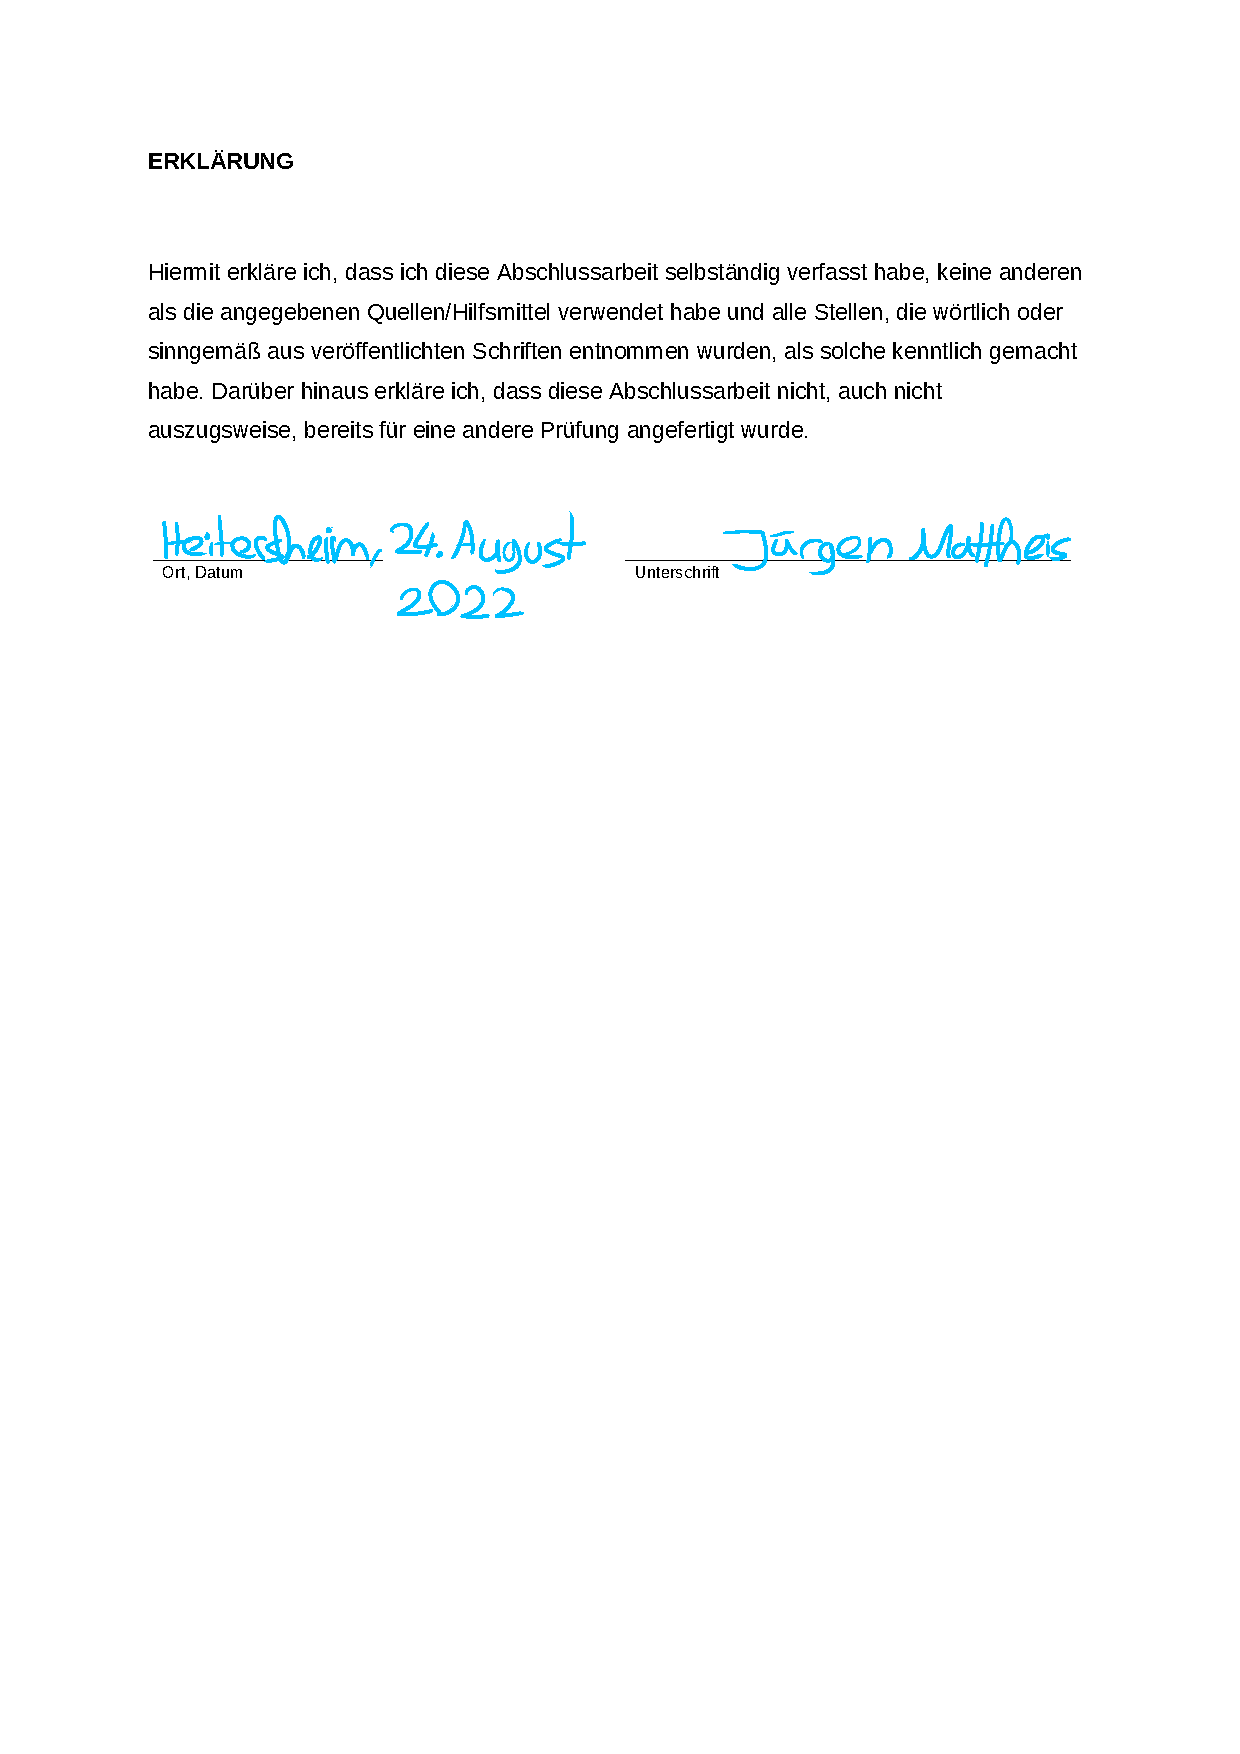
\includepdf[pages=-]{./ErklrungfrdieAbschlussarbeit_unterschrieben.pdf}

  \tableofcontents
  \listoffigures
  \listofcodecaptions
  \listoftables
  % https://tex.stackexchange.com/questions/538528/tcolorbox-newtcbtheorem-index-with-tcolorbox
  \tcblistof[\chapter*]{theorem_list}{Definitionsverzeichnis}
  % https://tex.stackexchange.com/questions/49155/how-can-i-list-items-created-with-the-float-package-in-the-toc
  \listof{floatgrammar}{Grammatikverzeichnis}

  \numberwithin{codecaption}{chapter}

  \newtcbtheorem[list inside={theorem_list},crefname={definition}{definitions}, number within=chapter]{Definition}{Definition}%
  {enhanced, arc=0mm,top=3mm,bottom=3mm, boxrule=0mm, borderline south={1mm}{0pt}{PrimaryColor}, title style={color=PrimaryColor},
  interior style={opacity=0.2, fill=PrimaryColor},
  frame style={color=white}, fonttitle=\bfseries, fontupper=\itshape,
  before upper=\setlength{\parskip}{1em}
  }{def}

  \newtcolorbox{Special_Paragraph}{enhanced, breakable, sharpish corners, notitle, arc=0mm, left=3mm, right=3mm, boxrule=1mm, borderline vertical={1mm}{0pt}{PrimaryColor},
  interior style={fill=SecondaryColor},
  frame style={color=white},
  % https://tex.stackexchange.com/questions/459870/paragraph-breaks-inside-tcolorbox, maybe also parbox=false
  before upper=\setlength{\parskip}{1em}
  }

  % https://tex.stackexchange.com/questions/319355/tcolorbox-breakable-option-not-working
  \newtcbinputlisting{\codebox}[2][]{
  listing file={#2},
  enhanced, colframe=PrimaryColor,colback=SecondaryColor, fonttitle=\bfseries, arc=0mm, bottom=1mm, top=1mm, left=1mm, right=1mm, #1, listing only, listing engine=minted, minted style=colorful, halign title=center, sharpish corners, drop fuzzy shadow, minted options={fontsize=\small,linenos=false,breaklines,breakafter={_}, breakbefore={(}, breakaftersymbolpre={}, breakaftersymbolpost={}, breakbeforesymbolpre={}, breakbeforesymbolpost={}, breaksymbolsepleft=2mm, breaksymbolsepright=0mm, breakindent=0mm, breaksymbolindentleft=5mm, breaksymbolindentright=0mm, numbersep=0mm}
  }
% drop fuzzy shadow, drop lifted shadow, listing engine=listings

  \newtcolorbox{Code_Frame}[2][]{enhanced, sharpish corners, drop fuzzy shadow, arc=0mm, bottom=1mm, top=1mm, left=1mm, right=1mm, boxrule=1mm, halign title=center, fonttitle=\bfseries, interior style={fill=white}, frame style={color=PrimaryColor}, title={#2}, #1}

  \newtcbinputlisting{\numberedcodebox}[2][]{
  listing file={#2},
  enhanced, breakable, colframe=PrimaryColor,colback=white, fonttitle=\bfseries, arc=0mm, #1, listing only, listing engine=minted, minted style=colorful, halign title=center, sharpish corners, drop fuzzy shadow, overlay={\begin{tcbclipinterior}\fill[PrimaryColor] (frame.south west) rectangle ([xshift=5mm]frame.north west);\end{tcbclipinterior}}
  }

  %!Tex Root = ../Main.tex
% ./Packete_und_Deklarationen.tex
\chapter{Motivation}
\label{ch:motivation}

\section{PicoC und RETI}
\section{Aufgabenstellung}
% erweitern des Compilers aus dem Bachelorprojekt
\section{Eigenheiten der Sprache C}
% Abhängigkeit von Typ von Variable usw.
% Designfehler
% Spiral Rule
% Specifier, die ganzen Begriffe aus calcourse
\section{Richtlinien}
% Email an Scholl
% exakt gleiche Präzidenzregeln
% kein unnötiger Schnickschnack
                      % ./content/Motivation.tex
  \include{./content/Einführung}                      % ./content/Einführung.tex
  %!Tex Root = ../Main.tex
% ./Packete_und_Deklarationen.tex
% ./Titlepage.tex
% ./Motivation.tex
% ./Einführung.tex
% ./Implementierung2_Pntr_Array.tex,
% ./Implementierung3_Struct_Derived.tex,
% ./Implementierung4_Fun.tex,
% ./Ergebnisse_und_Ausblick.tex

\chapter{Implementierung}
\label{ch:implementierung}

\section{Lexikalische Analyse}
\subsection{Teil der Konkretten Syntax für die Lexikalische Analyse}
\numberwithin{floatgrammar}{section}

\label{sec:lex_analyse_verwendung_von_lark}
% ./concrete_syntax_picoc.lark
\begin{grammar}[Teil der Konkretten Syntax der Sprache $L_{PicoC}$ für die Lexikalische Analyse in EBNF, Teil 1][H][gr:concrete_syntax_lex_teil_1]
  \toprule
  \firstcase{COMMENT}{\dq //\dq\enspace /[{\wedge}\backslash n]{*}/\gralt \dq {/*}\dq\enspace  /(.\mid \setminus n)*?/\enspace \dq {*/}\dq }{L\_Comment}
  \firstcase{RETI\_COMMENT.2}{\dq {//}\dq \dq \text{\textvisiblespace} \dq ? \dq \#\dq /[\wedge\backslash n]{*}/}{}
  \midrule
  \firstcase{DIG\_NO\_0}{\dq 1\dq \gralt \dq 2\dq \gralt \dq 3\dq \gralt \dq 4\dq \gralt \dq 5\dq}{L\_Arith}
  \otherform{\dq 6\dq \gralt \dq 7\dq \gralt \dq 8\dq \gralt \dq 9\dq}{}
  \firstcase{DIG\_WITH\_0}{\dq 0\dq \gralt DIG\_NO\_0}{}
  \firstcase{NUM}{\dq 0\dq \gralt DIG\_NO\_0 DIG\_WITH\_0*}{}
  \firstcase{ASCII\_CHAR}{\dq\text{\textvisiblespace} \dq ..\dq \sim\dq }{}
  \firstcase{CHAR}{\dq '\dq ASCII\_CHAR\dq '\dq }{}
  \firstcase{FILENAME}{ASCII\_CHAR+\dq .picoc\dq }{}
  \firstcase{LETTER}{\dq {a}\dq ..\dq {z}\dq \gralt \dq {A}\dq ..\dq {Z}\dq}{}
  \firstcase{NAME}{(LETTER\gralt \dq \_\dq )}{}
  & & \qquad(LETTER\gralt DIG\_WITH\_0\gralt \dq \_\dq )* & \\
  \firstcase{name}{NAME\gralt INT\_NAME\gralt CHAR\_NAME}{}
  \otherform{VOID\_NAME}{}
  \firstcase{NOT}{\dq \sim\dq }{}
  \firstcase{REF\_AND}{\dq \&\dq }{}
  \firstcase{un\_op}{SUB\_MINUS\gralt LOGIC\_NOT\gralt NOT}{}
  \otherform{MUL\_DEREF\_PNTR \gralt REF\_AND}{}
  \firstcase{MUL\_DEREF\_PNTR}{\dq {*}\dq }{}
  \firstcase{DIV}{\dq /\dq }{}
  \firstcase{MOD}{\dq \%\dq }{}
  \firstcase{prec1\_op}{MUL\_DEREF\_PNTR\gralt DIV\gralt MOD}{}
  \firstcase{ADD}{\dq {+}\dq }{}
  \firstcase{SUB\_MINUS}{\dq {-}\dq }{}
  \firstcase{prec2\_op}{ADD\gralt SUB\_MINUS}{}
  \midrule
  \firstcase{LT}{\dq {<}\dq }{L\_Logic}
  \firstcase{LTE}{\dq {<=}\dq }{}
  \firstcase{GT}{\dq {>}\dq }{}
  \firstcase{GTE}{\dq {>=}\dq }{}
  \firstcase{rel\_op}{LT\gralt LTE\gralt GT\gralt GTE}{}
  \firstcase{EQ}{\dq {==}\dq }{}
  \firstcase{NEQ}{\dq {!=}\dq }{}
  \firstcase{eq\_op}{EQ\gralt NEQ}{}
  \firstcase{LOGIC\_NOT}{\dq !\dq }{}
  \bottomrule
\end{grammar}

\begin{grammar}[Teil der Konkretten Syntax der Sprache $L_{PicoC}$ für die Lexikalische Analyse in EBNF, Teil 2][H][gr:concrete_syntax_lex_teil_2]
  \toprule
  \firstcase{INT\_DT.2}{\dq int\dq }{L\_Assign\_Alloc}
  \firstcase{INT\_NAME.3}{\dq int\dq\enspace (LETTER\gralt DIG\_WITH\_0\gralt \dq \_\dq )+}{}
  \firstcase{CHAR\_DT.2}{\dq char\dq }{}
  \firstcase{CHAR\_NAME.3}{\dq char\dq\enspace (LETTER\gralt DIG\_WITH\_0\gralt \dq \_\dq )+}{}
  \firstcase{VOID\_DT.2}{\dq void\dq }{}
  \firstcase{VOID\_NAME.3}{\dq void\dq\enspace (LETTER\gralt DIG\_WITH\_0\gralt \dq \_\dq )+}{}
  \firstcase{prim\_dt}{INT\_DT\gralt CHAR\_DT\gralt VOID\_DT}{}
  \bottomrule
\end{grammar}

% \begin{grammar}[\(\lambda\) calculus syntax][p][gr:ex1]
%   \firstcase{T}{\nonterm{V}}{Variable}
%   \otherform{(\nonterm{T}\ \nonterm{T})}{Application}
%   \otherform{\lambda \nonterm{V}\cdot\nonterm{T}}{Abstraction}
%   \firstcase{V}{x, y, \dots}{Variables}
% \end{grammar}
% \begin{grammar}[Advanced capabilities of \texttt{grammar.sty}][p][gr:ex2]
%   \firstcase{A}{\nonterm{T} \gralt \nonterm{V}}{Multiple option on a single line}
%   \highlight
%   \otherform{\nonterm{A}}{Highlighted form}
%   \downplay
%   \otherform{\nonterm{B}\gralt \nonterm{C}}{Downplayed form}
%   \otherform{\lochighlight{\nonterm{A}} \gralt \nonterm{B}}{Emphasize part of the line}
% \end{grammar}

% erwähnen, dass in Lark die Grammatiken L_Lex und L_Parse gemischt sind
% EBNF erwähnen
% (erwähnen, dass finalle Grammatik im Appendix)
\subsection{Basic Lexer}
\section{Syntaktische Analyse}
\label{sec:syntaktische_analyse}

\subsection{Teil der Konkretten Syntax für die Syntaktische Analyse}
% ./concrete_syntax_picoc.lark
% https://tex.stackexchange.com/questions/851/removing-spaces-between-words-in-math-mode
In \ref{gr:concrete_syntax_parser}

\begin{grammar}[Teil der Konkretten Syntax der Sprache $L_{PicoC}$ für die Syntaktische Analyse in EBNF, Teil 1][H][gr:concrete_syntax_parser]
  \toprule
	\downplay
  \firstcase{prim\_exp}{name\gralt NUM\gralt CHAR\gralt "("logic\_or")"}{L\_Arith +}
	\downplay
  \firstcase{post\_exp}{array\_subscr\gralt struct\_attr\gralt fun\_call}{L\_Array +}
	\downplay
  \otherform{input\_exp\gralt print\_exp\gralt prim\_exp}{L\_Pntr +}
	\downplay
  \firstcase{un\_exp}{un\_op un\_exp\gralt post\_exp}{L\_Struct + L\_Fun}
  \midrule
	\downplay
  \firstcase{input\_exp}{\dq input\dq\dq(\dq\dq)\dq}{L\_Arith}
	\downplay
  \firstcase{print\_exp}{\dq print\dq\dq(\dq logic\_or\dq)\dq}{}
	\downplay
  \firstcase{arith\_prec1}{arith\_prec1\enspace prec1\_op\enspace un\_exp\gralt un\_exp}{}
	\downplay
  \firstcase{arith\_prec2}{arith\_prec2\enspace prec2\_op\enspace arith\_prec1\gralt arith\_prec1}{}
	\downplay
  \firstcase{arith\_and}{arith\_and\enspace \dq\&\dq\enspace arith\_prec2\gralt arith\_prec2}{}
	\downplay
  \firstcase{arith\_oplus}{arith\_oplus\enspace \dq {\wedge{}}\dq\enspace arith\_and\gralt arith\_and}{}
	\downplay
  \firstcase{arith\_or}{arith\_or\enspace \dq{\mid} \dq\enspace arith\_oplus\gralt arith\_oplus}{}
  \midrule
  \downplay
  \firstcase{rel\_exp}{rel\_exp\enspace rel\_op\enspace arith\_or\gralt arith\_or}{L\_Logic}
  \downplay
  \firstcase{eq\_exp}{eq\_exp\enspace eq\_op rel\_exp\gralt rel\_exp}{}
  \downplay
  \firstcase{logic\_and}{logic\_and\enspace \dq{\&\&}\dq\enspace eq\_exp\gralt eq\_exp}{}
  \downplay
  \firstcase{logic\_or}{logic\_or\enspace \dq{\mid\mid}\dq\enspace logic\_and\gralt logic\_and}{}
  \midrule
	\downplay
  \firstcase{type\_spec}{prim\_dt\gralt struct\_spec}{L\_Assign\_Alloc}
	\downplay
  \firstcase{alloc}{type\_spec\enspace pntr\_decl}{}
	\downplay
  \firstcase{assign\_stmt}{un\_exp\enspace \dq {=}\dq\enspace logic\_or\dq ;\dq }{}
  \firstcase{initializer}{logic\_or\gralt array\_init\gralt struct\_init}{}
	\downplay
  \firstcase{init\_stmt}{alloc\enspace \dq {=}\dq\enspace initializer\dq ;\dq }{}
	\downplay
  \firstcase{const\_init\_stmt}{\dq const\dq\enspace type\_spec\enspace name\enspace \dq {=}\dq\enspace NUM\dq ;\dq }{}
  \midrule
  \firstcase{pntr\_deg}{\dq {*}\dq *}{L\_Pntr}
  \firstcase{pntr\_decl}{pntr\_deg\enspace array\_decl\gralt array\_decl}{}
  \midrule
  \firstcase{array\_dims}{(\dq [\dq NUM\dq ]\dq )*}{L\_Array}
  \firstcase{array\_decl}{name\enspace array\_dims\gralt \dq (\dq pntr\_decl\dq )\dq  array\_dims}{}
  \firstcase{array\_init}{\dq \{\dq initializer(\dq ,\dq\enspace initializer)*\dq \}\dq }{}
  \firstcase{array\_subscr}{post\_exp\dq [\dq logic\_or\dq ]\dq }{}
  \midrule
  \firstcase{struct\_spec}{\dq struct\dq\enspace name}{L\_Struct}
  \firstcase{struct\_params}{(alloc\dq ;\dq )+}{}
  \firstcase{struct\_decl}{\dq struct\dq\enspace name\enspace \dq \{\dq struct\_params\dq \}\dq }{}
  \firstcase{struct\_init}{\dq \{\dq \dq .\dq name\dq {=}\dq initializer}{}
  & & \qquad(\dq ,\dq\enspace \dq .\dq name\dq {=}\dq initializer)*\dq \}\dq & \\
  \firstcase{struct\_attr}{post\_exp\dq .\dq name}{}
  \midrule
	\downplay
  \firstcase{if\_stmt}{\dq if\dq \dq (\dq logic\_or\dq )\dq\enspace exec\_part}{L\_If\_Else}
	\downplay
  \firstcase{if\_else\_stmt}{\dq if\dq \dq (\dq logic\_or\dq )\dq\enspace exec\_part\enspace \dq else\dq\enspace exec\_part}{}
  \midrule
	\downplay
  \firstcase{while\_stmt}{\dq while\dq \dq (\dq logic\_or\dq )\dq\enspace exec\_part}{L\_Loop}
	\downplay
  \firstcase{do\_while\_stmt}{\dq do\dq\enspace exec\_part\enspace \dq while \dq \dq (\dq logic\_or\dq )\dq \dq ;\dq }{}
  \bottomrule
\end{grammar}

\begin{grammar}[Teil der Konkretten Syntax der Sprache $L_{PicoC}$ für die Syntaktische Analyse in EBNF, Teil 2][H]
  \toprule
	\downplay
  \firstcase{decl\_exp\_stmt}{alloc\dq ;\dq }{L\_Stmt}
	\downplay
  \firstcase{decl\_direct\_stmt}{ assign\_stmt\gralt init\_stmt\gralt const\_init\_stmt}{}
  \firstcase{decl\_part}{ decl\_exp\_stmt\gralt decl\_direct\_stmt\gralt RETI\_COMMENT}{}
  \\[-0.2cm]
	\downplay
  \firstcase{compound\_stmt}{ \dq \{\dq exec\_part* \dq \}\dq }{}
	\downplay
  \firstcase{exec\_exp\_stmt}{logic\_or\dq ;\dq }{}
	\downplay
  \firstcase{exec\_direct\_stmt}{if\_stmt\gralt if\_else\_stmt\gralt while\_stmt\gralt do\_while\_stmt}{}
	\downplay
  \otherform{assign\_stmt\gralt fun\_return\_stmt}{}
  \firstcase{exec\_part}{compound\_stmt\gralt exec\_exp\_stmt\gralt exec\_direct\_stmt}{}
  \otherform{RETI\_COMMENT}{}
  \\[-0.2cm]
  \firstcase{decl\_exec\_stmts}{decl\_part* exec\_part*}{}
  \midrule
  \firstcase{fun\_args}{[logic\_or(\dq ,\dq\enspace logic\_or)*]}{L\_Fun}
  \firstcase{fun\_call}{name\dq (\dq fun\_args\dq )\dq }{}
  \firstcase{fun\_return\_stmt}{\dq return\dq\enspace [logic\_or]\dq ;\dq }{}
  \firstcase{fun\_params}{[alloc(\dq ,\dq\enspace alloc)*]}{}
  \firstcase{fun\_decl}{type\_spec\enspace pntr\_deg\enspace name\dq (\dq fun\_params\dq )\dq }{}
  \firstcase{fun\_def}{type\_spec\enspace pntr\_deg\enspace name\dq (\dq fun\_params\dq )\dq\enspace \dq \{\dq  decl\_exec\_stmts \dq \}\dq }{}
  \midrule
  \firstcase{decl\_def}{(struct\_decl\gralt fun\_decl)\dq ;\dq \gralt fun\_def}{L\_File}
  \firstcase{decls\_defs}{decl\_def*}{}
  \firstcase{file}{FILENAME\enspace decls\_defs}{}
  \bottomrule
\end{grammar}
% Vorteile von Lark
\subsection{Umsetzung von Präzidenz}
Die \colorbold{PicoC} Programmiersprache hat dieselben \colorbold{Präzidenzregeln} implementiert, wie die Programmiersprache \colorbold{C} \footcite{noauthor_c_nodate}. Die \colorbold{Präzidenzregeln} von \colorbold{PicoC} sind in Tabelle~\ref{tab:reference_table} aufgelistet.

% \rowcolors{2}{SecondaryColor}{white}
\begin{table}[H]
  \center
  % \Block{2}{=}{Links, dann rechts $\rightarrow$} \\
  \begin{NiceTabular}{X[1,c]X[2,c]X[3,l]X[2,c]}[rules/color=PrimaryColor] % {\linewidth}{|C|C|L|L|}
  \CodeBefore
  \rowcolor{PrimaryColor}{1}
  \rowcolors{2-18}{SecondaryColor}{}[cols={2-3}]
  \rowcolors{2-18}{SecondaryColor}{}[cols={1,4}, respect-blocks, restart]
  \Body
  \textbf{\textcolor{white}{Präzidenz}} &	\textbf{\textcolor{white}{Operator}} & \textbf{\textcolor{white}{Beschreibung}} &	\textbf{\textcolor{white}{Assoziativität}} \\
  1	& \verb|a()|	& Funktionsaufruf & \Block{3-1}{Links, dann rechts $\rightarrow$} \\
    & \verb|a[]|	& Indexzugriff & \\
    & \verb|a.b| & Attributzugriff & \\
  2	&	\verb|-a| & Unäres Minus & \Block{3-1}{Rechts, dann links $\leftarrow$} \\
    & \smalltt{!a $\thicksim$a}	& Logisches NOT und Bitweise NOT & \\
    & \verb|*a &a| & Dereferenz und Referenz, auch Adresse-von & \\
  3	& \smalltt{a*b a/b a\%b} &	Multiplikation, Division und Modulo & \Block{9-1}{Links, dann rechts $\rightarrow$} \\
  4	& \verb|a+b a-b|	& Addition und Subtraktion & \\
  5	& \verb|a<b a<=b| \verb|a>b a>=b| & Kleiner, Kleiner Gleich, Größer, Größer gleich & \\
  6 &	\verb|a==b a!=b| & Gleichheit und Ungleichheit & \\
  7 &	\verb|a&b| & Bitweise UND & \\
  8 &	\verb|a^b| & Bitweise XOR (exclusive or) & \\
  9 & \smalltt{a$\mid$b} & Bitweise ODER (inclusive or) & \\
  10	& \verb|a&&b| &	Logiches UND & \\
  11	& $a{\mid\mid} b$	& Logisches ODER & \\
  12 & \verb|a=b| & Zuweisung & Rechts, dann links $\leftarrow$ \\
  13 &	\verb|a,b|& Komma	& Links, dann rechts $\rightarrow$ \\
  \bottomrule
\end{NiceTabular}
\caption{Präzidenzregeln von PicoC}
\label{tab:reference_table}
\end{table}
% erwähnen von Mehrdeutigkeit und Assoziativität
% finalle Grammatik im Appendix
% Crafting Compilers Quelle benennen

\subsection{Derivation Tree Generierung}
\subsubsection{Early Parser}
\subsubsection{Codebeispiel}
\label{sec:derivation_tree_generierung}
\begin{code}
  \centering
  \numberedcodebox[minted language=c]{./code_examples/example_dt_simple_ast_gen_array_decl_and_alloc.picoc}
  \caption{PicoC Code für Derivation Tree Generierung}
  \label{code:picoc_code_für_derivation_tree_generierung}
\end{code}

\begin{code}
  \centering
  \numberedcodebox[minted language=text]{./code_examples/example_dt_simple_ast_gen_array_decl_and_alloc.dt}
  \caption{Derivation Tree nach Derivation Tree Generierung}
  \label{code:derivation_tree_nach_derivation_tree_generierung}
\end{code}

\subsection{Derivation Tree Vereinfachung}
\subsubsection{Visitor}
\subsubsection{Codebeispiel}

Beispiel aus Subkapitel~\ref{sec:derivation_tree_generierung} wird fortgeführt.

\begin{code}
  \centering
  \numberedcodebox[minted language=text]{./code_examples/example_dt_simple_ast_gen_array_decl_and_alloc.dt_simple}
  \caption{Derivation Tree nach Derivation Tree Vereinfachung}
  \label{code:picoc_code_nach_derivation_tree_vereinfachung}
\end{code}

% Visitor erwähnen
\subsection{Abstrakt Syntax Tree Generierung}
\subsubsection{PicoC-Knoten}
% Tabelle aller PicoC Knoten
% möglichst kurze und leicht verständliche Bezeichner für Knoten

\begin{table}[H]
  \center
  \begin{NiceTabular}{X[7]X[10]}[rules/color=PrimaryColor]
  \CodeBefore
  \rowcolor{PrimaryColor}{1}
  \rowcolors{2-17}{SecondaryColor}{}[cols={1-2}]
  \Body
  \textbf{\textcolor{white}{PiocC-Knoten}} & \textbf{\textcolor{white}{Beschreibung}} \\
  \smalltt{Name(val)} & Ein \colorbold{Bezeichner}, z.B. \smalltt{my\_fun, my\_var} usw. , aber da es keine gute Kurzform für \smalltt{Identifier()} (englisches Wort für Bezeichner) gibt, wurde dieser Knoten \smalltt{Name()} genannt. \\
  \smalltt{Num(val)} & Eine \colorbold{Zahl}, z.B. \smalltt{42, -3} usw. \\
  \smalltt{Char(val)} & Ein \colorbold{Zeichen} der \colorbold{ASCII-Zeichenkodierung}, z.B. \smalltt{'c', '*'} usw. \\
  \smalltt{Minus(), Not(), DerefOp(), RefOp(), LogicNot()} & Die \colorbold{unären Operatoren} \smalltt{un\_op}: \smalltt{-a, {$\thicksim$}a, *a, \&a !a}. \\
  \smalltt{Add(), Sub(), Mul(), Div(), Mod(), Oplus(), And(), Or(), LogicAnd(), LogicOr()} & Die \colorbold{binären Operatoren} \smalltt{bin\_op}: \smalltt{a + b, a - b, a * b, a / b, a \% b, a $\wedge$ b, a \& b, a $\mid$ b, a \&\& b, a {$\mid\mid$} b}. \\
  \smalltt{Eq(), NEq(), Lt(), LtE(), Gt(), GtE()} & Die \colorbold{Relationen} \smalltt{rel}: \smalltt{a == b, a != b, a < b, a <= b, a > b, a >= b}. \\
  \smalltt{Const(), Writeable()} & Die \colorbold{Type Qualifier} \smalltt{type\_qual}: \smalltt{const}, was für ein \colorbold{nicht beschreibbare} \colorbold{Konstante} steht und das \colorbold{nicht} Angeben von \smalltt{const}, was für einen \colorbold{beschreibbare} Variable steht. \\
\smalltt{IntType(), CharType(), VoidType()} & Die \colorbold{Type Specifier} für \colorbold{Primitiven Datentypen}, die in der Abstrakten Syntax, um eine intuitive Bezeichnung zu haben einfach nur unter \colorbold{Datentypen} \smalltt{datatype} eingeordnet werden: \smalltt{int},  \smalltt{char},  \smalltt{void}. \\
\smalltt{Placeholder()} & \colorbold{Platzhalter} für einen Knoten, der diesen später \colorbold{ersetzt}. \\
  \smalltt{BinOp(exp, bin\_op, exp)} & Container für eine \colorbold{binäre Operation} mit $2$ Expressions: \smalltt{<exp1> <bin\_op> <exp2>}\\
  \smalltt{UnOp(un\_op, exp)} & Container für eine \colorbold{unäre Operation} mit einer Expression: \smalltt{<un\_op> <exp>}. \\
  \smalltt{Exit(num)} & Container für einen \colorbold{Exit Code}, der vor der Beendigung in das \smalltt{ACC} Register geschrieben wird und steht für die \colorbold{Beendigung} des laufenden Programmes. \\
  \smalltt{Atom(exp, rel, exp)} & Container für eine \colorbold{binäre Relation} mit $2$ Expressions: \smalltt{<exp1> <rel> <exp2>}\\
  \smalltt{ToBool(exp)} & Container für einen \colorbold{Arithmetischen Ausdruck}, wie z.B. \smalltt{1 + 3} oder einfach nur \smalltt{3}, der nicht nur $1$ oder $0$ als Ergebnis haben kann und daher bei einem Ergebnis $x > 1$ auf $1$ abgebildet wird. \\
  \smalltt{Alloc(type\_qual, datatype, name, \textcolor{gray!90!black}{local\_var\_or\_param})} & \colorbold{Container} für eine \colorbold{Allokation} \smalltt{<type\_qual> <datatype> <name>} mit den notwendigen Knoten \smalltt{type\_qual},  \smalltt{datatype} und  \smalltt{name}, die alle für einen Eintrag in der  \colorbold{Symboltabelle} notwendigen Informationen enthalten. Zudem besitzt er ein \textcolor{gray!90!black}{verstecktes Attribut}  \smalltt{local\_var\_or\_param}, dass die Information trägt, ob es sich bei der \colorbold{Variable} um eine \colorbold{Lokale Variable} oder einen \colorbold{Parameter} handelt. \\
  \smalltt{Assign(lhs, exp)} & Container für eine \colorbold{Zuweisung}, wobei \smalltt{lhs} ein  \smalltt{Subscr(exp1, exp2)}, \smalltt{Deref(exp1, exp2)}, \smalltt{Attr(exp, name)} oder  \smalltt{Name('var')} sein kann und  \smalltt{exp} ein beliebiger \colorbold{Logischer Ausdruck} sein kann: \smalltt{lhs = exp}. \\
  \bottomrule
\end{NiceTabular}
\caption{PicoC-Knoten Teil 1}
\label{tab:picoc_knoten_teil_1}
\end{table}

\begin{table}[H]
  \center
  \begin{NiceTabular}{X[7]X[10]}[rules/color=PrimaryColor]
  \CodeBefore
  \rowcolor{PrimaryColor}{1}
  \rowcolors{2-13}{SecondaryColor}{}[cols={1-2}]
  \Body
  \textbf{\textcolor{white}{PiocC-Knoten}} & \textbf{\textcolor{white}{Beschreibung}} \\
  \smalltt{Exp(exp, \textcolor{gray!90!black}{datatype}, \textcolor{gray!90!black}{error\_data})} & Container für einen \colorbold{beliebigen Ausdruck}, dessen Ergebnis auf den \colorbold{Stack} soll. Zudem besitzt er $2$ \textcolor{gray!90!black}{versteckte Attribute}, wobei \smalltt{datatype} im \colorbold{RETI Blocks Pass} wichtig ist und \smalltt{error\_data} für \colorbold{Fehlermeldungen} wichtig ist. \\
  \smalltt{Stack(num)} & Container, der für das \colorbold{temporäre} Ergebnis einer Berechnung, das \smalltt{num} Speicherzellen relativ zum  \colorbold{Stackpointer Register} \smalltt{SP} steht.\\
  \smalltt{Stackframe(num)} & Container, der für eine Variable steht, die \smalltt{num} Speicherzellen relativ zum \colorbold{Begin-Aktive-Funktion Register} \smalltt{BAF} steht. \\
  \smalltt{Global(num)} & Container, der für eine Variable steht, die \smalltt{num} Speicherzellen relativ zum \colorbold{Datensegment Register} \smalltt{DS} steht. \\
  \smalltt{StackMalloc(num)} & Container, der für das \colorbold{Allokieren} von \smalltt{num} Speicherzellen auf dem \colorbold{Stack} steht. \\
\smalltt{PntrDecl(num, datatype)} & Container, der für den \colorbold{Pointerdatentyp} steht: \smalltt{<prim\_dt> *<var>}, wobei das \colorbold{Attribut} \smalltt{num} die \colorbold{Anzahl zusammengefasster Pointer} angibt und \smalltt{datatype} der {Datentyp} ist, auf den der oder die \colorbold{Pointer} zeigen. \\
\smalltt{Ref(exp, \textcolor{gray!90!black}{datatype}, \textcolor{gray!90!black}{error\_data})} & Container, der für die Anwendung des \colorbold{Referenz-Operators} \smalltt{\&<var>} steht und die \colorbold{Adresse} einer \colorbold{Location} (Definition~\ref{def:location}) auf den Stack schreiben soll, die über \smalltt{exp} eingegrenzt wird. Zudem besitzt er $2$ \textcolor{gray!90!black}{versteckte Attribute}, wobei \smalltt{datatype} im \colorbold{RETI Blocks Pass} wichtig ist und \smalltt{error\_data} für \colorbold{Fehlermeldungen} wichtig ist. \\
\smalltt{Deref(lhs, exp)} & Container für den \colorbold{Indexzugriff} auf einen \colorbold{Array-} oder \colorbold{Pointerdatentyp}: \smalltt{<var>[<i>]}, wobei \smalltt{exp1} eine angehängte weitere \smalltt{Subscr(exp1, exp2)}, \smalltt{Deref(exp1, exp2)}, \smalltt{Attr(exp, name)} oder ein \smalltt{Name('var')} sein kann und \smalltt{exp2} der Index ist auf den zugegriffen werden soll. \\
\smalltt{ArrayDecl(nums, datatype)} & Container, der für den \colorbold{Arraydatentyp} steht: \smalltt{<prim\_dt> <var>[<i>]}, wobei das \colorbold{Attribut} \smalltt{nums} eine Liste von \smalltt{Num('x')} ist, die die \colorbold{Dimensionen} des Arrays angibt und \smalltt{datatype} der {Datentyp} ist, der über das Anwenden von \smalltt{Subscript()} auf das Array zugreifbar ist. \\
\smalltt{Array(exps, \textcolor{gray!90!black}{datatype})} & Container für den \colorbold{Initializer} eines \colorbold{Arrays}, dessen Einträge \smalltt{exps} weitere Initializer für eine \colorbold{Array-Dimension} oder ein Initializer für ein \colorbold{Struct} oder ein \colorbold{Logischer Ausdruck} sein können, z.B. \smalltt{\{\{1, 2\}, \{3, 4\}\}}. Des Weiteren besitzt er ein \textcolor{gray!90!black}{verstecktes Attribut} \smalltt{datatype}, welches für den \colorbold{PicoC-ANF Pass} Informationen transportiert, die für \colorbold{Fehlermeldungen} wichtig sind. \\
\smalltt{Subscr(exp1, exp2)} & Container für den \colorbold{Indexzugriff} auf einen \colorbold{Array-} oder \colorbold{Pointerdatentyp}: \smalltt{<var>[<i>]}, wobei \smalltt{exp1} eine angehängte weitere \smalltt{Subscr(exp1, exp2)}, \smalltt{Deref(exp1, exp2)} oder \smalltt{Attr(exp, name)} Operation sein kann oder ein \smalltt{Name('var')} sein kann und \smalltt{exp2} der Index ist auf den zugegriffen werden soll. \\
  \smalltt{StructSpec(name)} & Container für einen selbst definierten \colorbold{Structdatentyp}: \smalltt{struct <name>}, wobei das \colorbold{Attribut} \smalltt{name} festlegt, welchen \colorbold{selbst definierte} Structdatentyp dieser Container-Knoten repräsentiert. \\
  \smalltt{Attr(exp, name)} & Container für den \colorbold{Attributzugriff} auf einen \colorbold{Structdatentyp}: \smalltt{<var>.<attr>}, wobei \smalltt{exp1} eine angehängte weitere \smalltt{Subscr(exp1, exp2)}, \smalltt{Deref(exp1, exp2)} oder \smalltt{Attr(exp, name)} Operation sein kann oder ein \smalltt{Name('var')} sein kann und \smalltt{name} das Attribut ist, auf das zugegriffen werden soll. \\
  \bottomrule
\end{NiceTabular}
\caption{PicoC-Knoten Teil 2}
\label{tab:picoc_knoten_teil_2}
\end{table}

\begin{table}[H]
  \center
  \begin{NiceTabular}{X[7]X[10]}[rules/color=PrimaryColor]
  \CodeBefore
  \rowcolor{PrimaryColor}{1}
  \rowcolors{2-9}{SecondaryColor}{}[cols={1-2}]
  \Body
  \textbf{\textcolor{white}{PiocC-Knoten}} & \textbf{\textcolor{white}{Beschreibung}} \\
  \smalltt{Struct(assigns, \textcolor{gray!90!black}{datatype})} & Container für den \colorbold{Initializer} eines \colorbold{Structs}, z.B \smalltt{\{.<attr1>=\{1, 2\}, .<attr2>=\{3, 4\}\}}, dessen Eintrag \smalltt{assigns} eine Liste von \smalltt{Assign(lhs, exp)} ist mit einer Zuordnung eines \colorbold{Attributezeichners}, zu einem weiteren Initializer für eine \colorbold{Array-Dimension} oder zu einem Initializer für ein \colorbold{Struct} oder zu einem \colorbold{Logischen Ausdruck}. Des Weiteren besitzt er ein  \textcolor{gray!90!black}{verstecktes Attribut} \smalltt{datatype}, welches für den \colorbold{PicoC-ANF Pass} Informationen transportiert, die für \colorbold{Fehlermeldungen} wichtig sind. \\
  \smalltt{StructDecl(name, allocs)} & Container für die Deklaration eines \colorbold{selbstdefinierten Structdatentyps}, z.B. \smalltt{struct <var> \{<datatype> <attr1>; <datatype> <attr2>;\};}, wobei \smalltt{name} der \colorbold{Bezeichner} des Structdatentyps ist und \smalltt{allocs} eine Liste von Bezeichnern der \colorbold{Attribute} des Structdatentyps mit dazugehörigem \colorbold{Datentyp}, wofür sich der \colorbold{Container-Knoten} \smalltt{Alloc(type\_qual, datatype, name)} sehr gut als \colorbold{Container} eignet. \\
  \smalltt{If(exp, stmts)} & Container für ein \colorbold{If Statement} \smalltt{if(<exp>) \{ <stmts> \}} inklusive  \colorbold{Condition}  \smalltt{exp} und einem  \colorbold{Branch}  \smalltt{stmts}, indem eine \colorbold{Liste von Statements} stehen kann oder ein einzelnes \smalltt{GoTo(Name('block.xyz'))}. \\
  \smalltt{IfElse(exp, stmts1, stmts2)} & Container für ein \colorbold{If-Else Statement} \smalltt{if(<exp>) \{ <stmts2> \} else \{ <stmts2> \}} inklusive \colorbold{Codition} \smalltt{exp} und $2$ \colorbold{Branches} \smalltt{stmts1} und \smalltt{stmts2}, die zwei Alternativen Darstellen in denen jeweils \colorbold{Listen von Statements} oder  \smalltt{GoTo(Name('block.xyz'))}'s stehen können. \\
  \smalltt{While(exp, stmts)} & Container für ein \colorbold{While-Statement} \smalltt{while(<exp>) \{ <stmts> \}} inklusive  \colorbold{Condition}  \smalltt{exp} und einem \colorbold{Branch}  \smalltt{stmts}, indem eine \colorbold{Liste von Statements} stehen kann oder ein einzelnes \smalltt{GoTo(Name('block.xyz'))}. \\
  \smalltt{DoWhile(exp, stmts)} & Container für ein \colorbold{Do-While-Statement} \smalltt{do \{ <stmts> \} while(<exp>);} inklusive  \colorbold{Condition}  \smalltt{exp} und einem \colorbold{Branch}  \smalltt{stmts}, indem eine \colorbold{Liste von Statements} stehen kann oder ein einzelnes \smalltt{GoTo(Name('block.xyz'))}. \\
  \smalltt{Call(name, exps)} & Container für einen \colorbold{Funktionsaufruf}: \smalltt{fun\_name(exps)}, wobei \smalltt{name} der \colorbold{Bezeichner} der Funktion ist, die aufgerufen werden soll und \smalltt{exps} eine \colorbold{Liste von Argumenten} ist, die an die Funktion übergeben werden soll. \\
  \smalltt{Return(exp)} & Container für ein \smalltt{Return-Statement}: \smalltt{return <exp>}, wobei das  \colorbold{Attribut}  \smalltt{exp} einen  \colorbold{Logischen Ausdruck} darstellt, dessen Ergebnis vom  \colorbold{Return-Statement} zurückgegeben wird. \\
  \smalltt{FunDecl(datatype, name, allocs)} & Container für eine \colorbold{Funktionsdeklaration}, z.B. \smalltt{<datatype> <fun\_name>(<datatype> <param1>, <datatype> <param2>)}, wobei \smalltt{datatype} der  \colorbold{Rückgabewert} der Funktion ist,  \smalltt{name} der  \colorbold{Bezeichner} der Funktion ist und \smalltt{allocs} die \colorbold{Parameter} der Funktion sind, wobei der \colorbold{Container-Knoten} \smalltt{Alloc(type\_spec, datatype, name)} als Cotainer für die Parameter dient. \\
  \bottomrule
\end{NiceTabular}
\caption{PicoC-Knoten Teil 3}
\label{tab:picoc_knoten_teil_3}
\end{table}

\begin{table}[H]
  \center
  \begin{NiceTabular}{X[7]X[10]}[rules/color=PrimaryColor]
  \CodeBefore
  \rowcolor{PrimaryColor}{1}
  \rowcolors{2-9}{SecondaryColor}{}[cols={1-2}]
  \Body
  \textbf{\textcolor{white}{PiocC-Knoten}} & \textbf{\textcolor{white}{Beschreibung}} \\
  \smalltt{FunDef(datatype, name, allocs, stmts\_blocks)} & Container für eine \colorbold{Funktionsdefinition}, z.B. \smalltt{<datatype> <fun\_name>(<datatype> <param>) \{<stmts>\}}, wobei \smalltt{datatype} der  \colorbold{Rückgabewert} der Funktion ist,  \smalltt{name} der  \colorbold{Bezeichner} der Funktion ist, \smalltt{allocs} die \colorbold{Parameter} der Funktion sind, wobei der \colorbold{Container-Knoten} \smalltt{Alloc(type\_spec, datatype, name)} als Cotainer für die Parameter dient und \smalltt{stmts\_blocks} eine Liste von \colorbold{Statemetns} bzw.  \colorbold{Blöcken} ist, welche diese Funktion beinhaltet. \\
  \smalltt{NewStackframe(fun\_name, goto\_after\_call)} & Container für die \colorbold{Erstellung} eines neuen \colorbold{Stackframes} und Speicherung des Werts des \smalltt{BAF}-Registers der \colorbold{aufrufenden Funktion} und der \colorbold{Rücksprungadresse} nacheinander an den \colorbold{Anfang} des neuen \colorbold{Stackframes}. Das Attribut \smalltt{fun\_name} stehte dabei für den Bezeichner der Funktion, für die ein neuer \colorbold{Stackframe} erstellt werden soll. Das Attribut \smalltt{fun\_name} dient später dazu den \colorbold{Block} dieser Funktion zu finden, weil dieser für den weiteren Kompiliervorang wichtige Information in seinen \textcolor{gray!90!black}{versteckte Attributen} gespeichert hat. Des Weiteren ist das Attribut \smalltt{goto\_after\_call} ein \smalltt{GoTo(Name('addr@next\_instr'))}, welches später durch die \colorbold{Adresse} des Befehls, der direkt auf die \colorbold{Jump Instruction} folgt, ersetzt wird.\\
  \smalltt{RemoveStackframe()} & Container für das \colorbold{Entfernen} des aktuellen \colorbold{Stackframes} durch das \colorbold{Wiederherstellen} des im noch \colorbold{aktuellen Stackframe} gespeicherten Werts des \smalltt{BAF}-Registes der \colorbold{aufrufenden Funktion} und das Setzen des \smalltt{SP}-Registers auf den Wert des \smalltt{BAF}-Registesr \colorbold{vor} der Wiederherstellung. \\
  \smalltt{File(name, decls\_defs\_blocks)} & Container für alle \colorbold{Funkionen} oder \colorbold{Blöcke}, welche eine Datei als Ursprung haben, wobei \smalltt{name} der \colorbold{Dateiname} der Datei ist, die erstellt wird und \smalltt{decls\_defs\_blocks} eine Liste von \colorbold{Funktionen} bzw. \colorbold{Blöcken} ist. \\
  \smalltt{Block(name, stmts\_instrs, \textcolor{gray!90!black}{instrs\_before}, \textcolor{gray!90!black}{num\_instrs}, \textcolor{gray!90!black}{param\_size}, \textcolor{gray!90!black}{local\_vars\_size})} & Container für \colorbold{Statements}, der auch als \colorbold{Block} bezeichnet wird, wobei das Attribut \smalltt{name} der Bezeichners des \colorbold{Labels} (Definition~\ref{def:label}) des Blocks ist und \smalltt{stmts\_instrs} eine \colorbold{Liste von Statements} oder \colorbold{Instructions}. Zudem besitzt er noch $3$ \textcolor{gray!90!black}{versteckte Attribute}, wobei  \smalltt{instrs\_before} die Zahl der \colorbold{Instructions} vor diesem \colorbold{Block} zählt,  \smalltt{num\_instrs} die Zahl der Instructions ohne Kommentare in diesem Block zählt, \smalltt{param\_size} die voraussichtliche Anzahl an Speicherzellen aufaddiert, die für die \colorbold{Parameter} der Funktion belegt werden müssen und \smalltt{local\_vars\_size} die voraussichtliche Anzahl an Speicherzellen aufaddiert, die für die \colorbold{lokalen Variablen} der Funktion belegt werden müssen. \\
  \smalltt{GoTo(name)} & Container für ein \smalltt{Goto} zu einem anderen \colorbold{Block}, wobei das Attribut \smalltt{name} der Bezeichner des \colorbold{Labels} des Blocks ist zu dem Gesprungen werden soll. \\
  \smalltt{SingleLineComment(prefix, content)} & Container für einen \colorbold{Kommentar}, den der Compiler selber während des \colorbold{Kompiliervorangs} erstellt, der im \colorbold{RETI-Interpreter} selbst später \colorbold{nicht} sichtbar sein wird, aber in den \colorbold{Immediate}-Dateien, welche die \colorbold{Abstract Syntax Trees} nach den verschiedenen \colorbold{Passes} enthalten. \\
  \smalltt{RETIComment(value)} & Container für einen \colorbold{Kommentar} im Code der Form: \smalltt{// \# comment}, der im \colorbold{RETI-Intepreter} später sichtbar sein wird und zur Orientierung genutzt werden kann, allerdings in einer tatsächlichen Implementierung einer \colorbold{RETI-CPU} \colorbold{nicht umsetzbar} ist und auch nicht sinnvoll wäre umzusetzen. Der \colorbold{Kommentar} ist im Attribut \colorbold{value}, welches jeder Knoten besitzt gespeichert. \\
  \bottomrule
\end{NiceTabular}
\caption{PicoC-Knoten Teil 4}
\label{tab:picoc_knoten_teil_4}
\end{table}


\begin{Definition}{Label}{label}
  Durch einen \colorbold{Bezeichner} \colorbold{eindeutig} zuordenbares \colorbold{Sprungziel} im Programmcode.\footcite{thiemann_compilerbau_2021}
\end{Definition}

\begin{Special_Paragraph}
  Die \textcolor{gray!90!black}{ausgegrauten} Attribute der PicoC-Nodes sind \textcolor{gray!90!black}{versteckte Attribute}, die \colorbold{nicht} direkt bei der Erstellung der  \colorbold{PicoC-Nodes} mit einem Wert \colorbold{initialisiert} werden, sondern im \colorbold{Verlauf der Kompilierung} beim Durchlaufen der verschiedenen Passes etwas zugewiesen bekommen, dass im weiteren Kompiliervorgang \colorbold{Informationen} transportiert, die später im Kompiliervorgang nicht mehr so leicht zugänglich wären.

  Jeder \colorbold{Knoten} hat darüberhinaus auch noch $2$ \colorbold{Attribute} \smalltt{value} und \smalltt{position}, wobei \colorbold{value} bei einem \colorbold{Token-Knoten} (Definition~\ref{def:token_knoten}) dem \colorbold{Tokenwert} des Tokens, welches es ersetzt entspricht und bei \colorbold{Container-Knoten} (Definition~\ref{def:container_knoten}) unbesetzt ist. Das \colorbold{Attribut} \smalltt{position} wird später für Fehlermeldungen gebraucht.
\end{Special_Paragraph}

\begin{Definition}{Token-Knoten}{token_knoten}
  Ersetzt ein \colorbold{Token} bei der Generierung des \colorbold{Abstract Syntax Tree}, damit der Zugriff auf Knoten des Abstract Syntax Tree möglichst \colorbold{simpel} ist und keine vermeidbaren Fallunterscheidungen gemacht werden müssen.

  \colorbold{Token-Knoten} entsprechen im Abstract Syntax Tree \colorbold{Blättern}.\footcite{thiemann_compilerbau_2021}
\end{Definition}

\begin{Definition}{Container-Knoten}{container_knoten}
  Dient als \colorbold{Container} für andere \colorbold{Container-Knoten} und \colorbold{Token-Knoten}. Die \colorbold{Container-Knoten} werden optimalerweise immer so gewählt, dass sie \colorbold{mehrere Produktionen} der \colorbold{Konkretten Syntax} abdecken, die einen \colorbold{gleichen Aufbau} haben und sich auch unter einem \colorbold{Überbegriff} zusammenfassen lassen.\footnote{Wie z.B. die verschiedenen \colorbold{Arithmetischen Ausdrücke}, wie z.B. \smalltt{1 {\%} 3} und \colorbold{Logischen Ausdrücke}, wie z.B. \smalltt{1 \&\& 2 < 3}, die einen gleichen Aufbau haben mit immer einer \colorbold{Operation} in der Mitte haben und $2$ \colorbold{Operanden} auf beiden Seiten und sich unter dem Überbegriff \colorbold{Binäre Operationen} zusammenfassen lassen.}

  \colorbold{Container-Knoten} entsprechen im Abstract Syntax Tree \colorbold{Inneren Knoten}.\footcite{thiemann_compilerbau_2021}
\end{Definition}

\subsubsection{RETI-Knoten}
\begin{table}[H]
  \center
  \begin{NiceTabular}{X[8]X[10]}[rules/color=PrimaryColor]
  \CodeBefore
  \rowcolor{PrimaryColor}{1}
  \rowcolors{2-16}{SecondaryColor}{}[cols={1-2}]
  \Body
  \textbf{\textcolor{white}{RETI-Knoten}} &	\textbf{\textcolor{white}{Beschreibung}} \\
  \smalltt{Program(name, instrs)} & Container für alle \colorbold{Instructions}: \smalltt{<name> <instrs>}, wobei \smalltt{name} der \colorbold{Dateiname} der Datei ist, die erstellt wird und \smalltt{instrs} eine \colorbold{Liste von Instructions} ist. \\
  \smalltt{Instr(op, args)} & Container für eine \colorbold{Instruction}: \smalltt{<op> <args>}, wobei \smalltt{op} eine \colorbold{Operation} ist und  \smalltt{args} eine \colorbold{Liste von Argumenten} für dieser Operation. \\
  \smalltt{Jump(rel, im\_goto)} & Container für eine \colorbold{Jump-Instruction}: \smalltt{JUMP<rel> <im>}, wobei \smalltt{rel} eine \colorbold{Relation} ist und \smalltt{im\_goto} ein \colorbold{Immediate Value} \smalltt{Im(val)} für die \colorbold{Anzahl an Speicherzellen}, um die relativ zur \colorbold{Jump-Instruction} gesprungen werden soll oder ein \smalltt{GoTo(Name('block.xyz'))}, das später im \colorbold{RETI-Patch Pass} durch einen passenden \colorbold{Immediate Value} ersetzt wird. \\
  \smalltt{Int(num)} & Container für einen \colorbold{Interruptaufruf}: \smalltt{INT <im>}, wobei \smalltt{num} die \colorbold{Interrruptvektornummer} (IVN) für die passende Speicherzelle in der \colorbold{Interruptvektortabelle} ist, in der die Adresse der \colorbold{Interrupt-Service-Routine} (ISR) steht. \\
  \smalltt{Call(name, reg)} & Container für einen \colorbold{Prozeduraufruf}: \smalltt{CALL <name> <reg>}, wobei \smalltt{name} der \colorbold{Bezeichner} der  Prozedur, die aufgerufen werden soll ist und \smalltt{reg} ein \colorbold{Register} ist, das als \colorbold{Argument} an die Prozedur dient. Diese \colorbold{Operation} ist in der Betriebssysteme Vorlesung\tabularnote{\cite{scholl_betriebssysteme_2020}} nicht deklariert, sondern wurde dazuerfunden, um unkompliziert ein  \smalltt{CALL PRINT ACC} oder  \smalltt{CALL INPUT ACC} im RETI-Interpreter simulieren zu können. \\
  \smalltt{Name(val)} & Bezeichner für eine \colorbold{Prozedur}, z.B. \smalltt{PRINT} oder \smalltt{INPUT} oder den \colorbold{Programnamen}, z.B. \smalltt{PROGRAMNAME}. Dieses \colorbold{Argument} ist in der Betriebssysteme Vorlesung\tabularnote{\cite{scholl_betriebssysteme_2020}} nicht deklariert, sondern wurde dazuerfunden, um Bezeichner, wie \smalltt{PRINT}, \smalltt{INPUT} oder \smalltt{PROGRAMNAME} schreiben zu können. \\
  \smalltt{Reg(reg)} & Container für ein \colorbold{Register}. \\
  \smalltt{Im(val)} & Ein \colorbold{Immediate Value}, z.B. \smalltt{42, -3} usw. \\
  \smalltt{Add(), Sub(), Mult(), Div(), Mod(), Oplus(), Or(), And()} & \colorbold{Compute-Memory} oder \colorbold{Compute-Register} Operationen: \smalltt{ADD, SUB, MULT, DIV, OPLUS, OR, AND}.\\
  \smalltt{Addi(), Subi(), Multi(), Divi(), Modi(), Oplusi(), Ori(), Andi()} & \colorbold{Compute-Immediate} Operationen: \smalltt{ADDI, SUBI, MULTI, DIVI, MODI, OPLUSI, ORI, ANDI}.\\
  \smalltt{Load(), Loadin(), Loadi()} & \colorbold{Load} Operationen: \smalltt{LOAD, LOADIN, LOADI}.\\
  \smalltt{Store(), Storein(), Move()} & \colorbold{Store} Operationen: \smalltt{STORE, STOREIN, MOVE}.\\
  \smalltt{Lt(), LtE(), Gt(), GtE(), Eq(), NEq(), Always(), NOp()} & \colorbold{Relationen}: \smalltt{<, <=, >, >=, ==, !=, \_NOP}.\\
  \smalltt{Rti()} & \colorbold{R}eturn-\colorbold{F}rom-\colorbold{I}nterrupt Operation: \smalltt{RTI}.\\
  \smalltt{Pc(), In1(), In2(), Acc(), Sp(), Baf(), Cs(), Ds()} & \colorbold{Register}: \smalltt{PC, IN1, IN2, ACC, SP, BAF, CS, DS}.\\
  \bottomrule
\end{NiceTabular}
\caption{RETI-Knoten}
\label{tab:reti_knoten}
\end{table}
% Tabelle aller RETI Knoten
% Transformer erwähnen

\subsubsection{Kompositionen von PicoC-Knoten und RETI-Knoten mit besonderer Bedeutung}
Hier sind jegliche \colorbold{Kompositionen} von \colorbold{PicoC-Knoten} und \colorbold{RETI-Knoten} aufgelistet, die eine \colorbold{besondere Bedeutung} haben und nicht bereits in der \colorbold{Abstrakten Syntax}~\ref{gr:concrete_syntax_parser} enthalten sind.
% (generelle Aufgaben von Exp und Reg)

\begin{table}[H]
  \center
  \begin{NiceTabular}{X[16]X[20]}[rules/color=PrimaryColor]
  \CodeBefore
  \rowcolor{PrimaryColor}{1}
  \rowcolors{2-15}{SecondaryColor}{}[cols={1-2}]
  \Body
  \textbf{\textcolor{white}{Komposition}} &	\textbf{\textcolor{white}{Beschreibung}} \\
  \smalltt{Ref(Global(Num('addr')))}	& Speichert \colorbold{Adresse} der Speicherzelle, die \smalltt{Num('addr')} Speicherzellen \colorbold{relativ} zum \colorbold{Datensegment Register} \smalltt{DS} steht auf den \colorbold{Stack}. \\
  \smalltt{Ref(Stackframe(Num('addr')))} & Speichert \colorbold{Adresse} der Speicherzelle, die \smalltt{Num('addr')} Speicherzellen \colorbold{relativ} zum \colorbold{Begin-Aktive-Funktion Register} \smalltt{BAF} steht auf den \colorbold{Stack}. \\
  \smalltt{Ref(Subscr(Stack(Num('addr1')), Stack(Num('addr2'))))} & Berechnet die nächste \colorbold{Adresse} aus der \colorbold{Adresse}, die an Speicherzelle \smalltt{Stack(Num('addr1'))} steht und dem \colorbold{Subscript Index}, der an Speicherzelle \smalltt{Stack(Num('addr2'))} steht und speichert diese auf den \colorbold{Stack}. Die Berechnung ist abhängig davon ob der \colorbold{Datentyp} \smalltt{ArrayDecl(datatype)} oder \smalltt{PntrDecl(datatype)} ist. Der \colorbold{Datentyp} ist ein \textcolor{gray!90!black}{verstecktes Attribut} von \smalltt{Ref(exp)}. \\
  \smalltt{Ref(Attr(Stack(Num('addr1')), Name('attr')))} & Berechnet die nächste \colorbold{Adresse} aus der \colorbold{Adresse}, die an Speicherzelle \smalltt{Stack(Num('addr1'))} steht und dem \colorbold{Attributnamen} \smalltt{Name('attr')} und speichert diese auf den \colorbold{Stack}. Zur Berechnung ist der Name des \colorbold{Struct} in \smalltt{StructSpec(Name('st'))} notwendig, dessen \colorbold{Attribut} \smalltt{Name('attr')} ist. \smalltt{StructSpec(Name('st'))} ist ein \textcolor{gray!90!black}{verstecktes Attribut} von  \smalltt{Ref(exp)}. \\
  \smalltt{Assign(Stack(Num('size'))), Global(Num('addr')))} & Schreibt \smalltt{Num('size')} viele Speicherzellen, die ab \smalltt{Global(Num('addr'))} relativ zum \colorbold{Datensegment Register}  \smalltt{DS} stehen, versetzt genauso auf den \colorbold{Stack}. \\
  \smalltt{Assign(Stack(Num('size')), Stackframe(Num('addr')))} & Schreibt \smalltt{Num('size')} viele Speicherzellen, die ab \smalltt{Stackframe(Num('addr'))} relativ zum \colorbold{Begin-Aktive-Funktion Register} \smalltt{BAF} stehen, versetzt genauso auf den \colorbold{Stack}. \\
  \smalltt{Exp(Global(Num('addr'))} & Speichert \colorbold{Inhalt} der Speicherzelle, die \smalltt{Num('addr')} Speicherzellen \colorbold{relativ} zum \colorbold{Datensegment Register} \smalltt{DS} steht auf den \colorbold{Stack}. \\
  \smalltt{Exp(Stackframe(Num('addr'))} & Speichert \colorbold{Inhalt} der Speicherzelle, die \smalltt{Num('addr')} Speicherzellen \colorbold{relativ} zum \colorbold{Begin-Aktive-Funktion Register} \smalltt{BAF} steht auf den \colorbold{Stack}. \\
  \smalltt{Exp(Stack(Num('addr')))} & Speichert \colorbold{Inhalt} der Speicherzelle, die \smalltt{Num('addr')} Speicherzellen \colorbold{relativ} zum \colorbold{Stackpointer Register}  \smalltt{SP} steht auf den \colorbold{Stack}. \\
  \smalltt{Assign(Stack(Num('addr1')), Stack(Num('addr2')))} & Speichert \colorbold{Inhalt} der Speicherzelle \smalltt{Stack(Num('addr2'))}, die \smalltt{Num('addr2')} Speicherzellen \colorbold{relativ} zum \colorbold{Stackpointer Register}  \smalltt{SP} steht an der \colorbold{Adresse} in der Speicherzelle, die \smalltt{Num('addr1')} Speicherzellen \colorbold{relativ} zum \colorbold{Stackpointer Register}  \verb|SP| steht. \\
  \smalltt{Assign(Global(Num('addr')), Stack(Num('size')))} & Schreibt \smalltt{Num('size')} viele Speicherzellen, die auf dem \colorbold{Stack} stehen, versetzt genauso auf die Speicherzellen ab \smalltt{Num('addr')} \colorbold{relativ} zum \colorbold{Datensegment Register}  \smalltt{DS}. \\
  \smalltt{Assign(Stackframe(Num('addr')), Stack(Num('size')))} & Schreibt \smalltt{Num('size')} viele Speicherzellen, die auf dem \colorbold{Stack} stehen, versetzt genauso auf die Speicherzellen ab \smalltt{Num('addr')} \colorbold{relativ} zum \colorbold{Begin-Aktive-Funktion Register} \smalltt{BAF}. \\
  \smalltt{Exp(Reg(reg))} & Schreibt den aktuellen Wert des \colorbold{Registers} \smalltt{reg} auf den \colorbold{Stack}. \\
  \smalltt{Instr(Loadi(), [Reg(Acc()), GoTo(Name('addr@next\_instr'))])} & Lädt in das Register \verb|ACC| die \colorbold{Adresse} der Instruction, die in diesem Kontext direkt nach dem Sprung zum Block einer anderen Funktion steht.\\
  \bottomrule
\end{NiceTabular}
\caption{Kompositionen von PicoC-Knoten und RETI-Knoten mit besonderer Bedeutung}
\label{tab:kompositionen_von_picoc_knoten_und_reti_knoten_mit_besonderer_bedeutung}
\end{table}

\begin{Special_Paragraph}
  Um die obige Tabelle~\ref{tab:kompositionen_von_picoc_knoten_und_reti_knoten_mit_besonderer_bedeutung} nicht mit unnötig viel repetetiven Inhalt zu füllen, wurden die zahlreichen Kompostionen \colorbold{ausgelassen}, bei denen einfach nur \verb|exp| durch $\mathtt{Stack(Num('x')), x}\in\mathbb{N}$ ersetzt wurde.

  Zudem sind auch jegliche Kombinationen ausgelassen, bei denen einfach nur eine \colorbold{Expression} an ein \smalltt{Exp(exp)} bzw.  \smalltt{Ref(exp)} drangehängt wurde.
\end{Special_Paragraph}

\subsubsection{Abstrakte Syntax}
\label{sec:abstrakte_syntax}

% ./abstract_syntax.txt
\newpage

\begin{grammar}[Abstrakte Syntax der Sprache $L_{PiocC}$][H][gr:abstract_syntax_l_picoc]
  \toprule
  \commentsecond
  \midrule
  \arith
  \midrule
  \logic
  \midrule
  \assign
  \midrule
  \pntr
  \midrule
  \arraysecond
  \midrule
  \struct
  \midrule
  \ifelse
  \midrule
  \loopsecond
  \midrule
  \fun
  \midrule
  \file
  \bottomrule
\end{grammar}

\begin{Special_Paragraph}
  Man spricht hier von der \colorbold{\enquote{Abstrakten Syntax der Sprache $L_{PicoC}$}} und meint hier mit der Sprache $L_{PicoC}$ \colorbold{nicht} die Sprache, welche durch die \colorbold{Abstrakte Syntax} beschrieben wird. Es ist damit \colorbold{immer} die Sprache gemeint, die \colorbold{kompiliert} werden soll und zu deren Zweck die \colorbold{Abstrakt Syntax} überhaupt definiert wird. Für die tatsächliche Sprache, die durch die \colorbold{Abstrakt Syntax} beschrieben wird, interessiert man sich nie wirklich explizit. Diese \colorbold{Redeart} wurde aus der \colorbold{Quelle} \cite{g_siek_course_2022} übernommen.
\end{Special_Paragraph}

% $L_{X}$ ist nicht notwendig sich zu überlegen, hier so getann als gäbe es diese Sprache
% Abstrakte Syntax ist für den Programmierer als Orientierungshilfe bei der Implementierung

\subsubsection{Transformer}
% Vielleicht Sache mit ToBool erwähnen aber vielleicht reicht es schon in der entsprechenden Tabelle
% Sache mit Deref und (), leftmost node
% Umdrehen von ArrayDecl und PntrDecl

\subsubsection{Ausgabe von Abstract Syntax Trees}
Ein \colorbold{Abstract Syntax Tree} kann entweder in der \colorbold{Konkretter Syntax} der Sprache, für dessen Kompilierung er generiert wurde oder in der \colorbold{Abstrakter Syntax}, die beschreibt, wie der Abstract Syntax Tree selbst aufgebaut sein darf ausgegeben werden.

Das Ausgeben eines \colorbold{Abstract Syntax Trees} wird im \colorbold{PicoC-Compiler} über die \colorbold{Magische Methode} \smalltt{\_\_repr\_\_()}\footnote{Spezielle Methode, die immer aufgerufen wird, wenn das \colorbold{Object}, dass in Besitz dieser Methode ist als \colorbold{String} mittels \smalltt{print()} oder zur \colorbold{Repräsentation} ausgegeben werden soll.} der Programmiersprache \colorbold{Python} umgesetzt. Sobald ein \colorbold{PicoC-Knoten} oder \colorbold{RETI-Knoten} ausgegeben werden soll, gibt seine Magische Methode \smalltt{\_\_repr\_\_()} eine nach der \colorbold{Abstrakten} oder \colorbold{Konkretten Syntax} aufgebaute \colorbold{Textrepräsentation} seiner selbst und all seiner Knoten mit an den richtigen Stellen passend gesetzten \colorbold{runden} \colorbold{öffnenden} \smalltt{(} und \colorbold{schließenden} \smalltt{)} \colorbold{Klammern}, sowie \colorbold{Kommas} \smalltt{','}, \colorbold{Semikolons} \smalltt{;} usw. zur Darstellung der \colorbold{Hierarchie} und zur \colorbold{Abtrennung} zurück. Dabei wird nach dem \colorbold{Depth-First-Search} Schema der gesamte \colorbold{Abstract Sybtax Tree} durchlaufen und die Magische \smalltt{\_\_repr\_\_()}-Methode der verschiedenen Knoten aufgerufen, die immer jeweils die \smalltt{\_\_repr\_\_()}-Methode ihrer Kinder aufrufen und die zurückgegebene \colorbold{Textrepräsentation} passend \colorbold{zusammenfügen} und selbst \colorbold{zurückgeben}.

Im \colorbold{PicoC-Compiler} wurden \colorbold{Abstrakte} und \colorbold{Konkrette Syntax} miteinander gemischt. Für \colorbold{PicoC-Knoten} wurde die \colorbold{Abstrakte Syntax} verwendet, da Passes schließlich auf \colorbold{Abstract Syntax Trees} operieren. Bei \colorbold{RETI-Knoten} wurde die \colorbold{Konkrette Syntax} verwendet, da \colorbold{Maschienenbefehle} in \colorbold{Konkretter Syntax} schließlich das \colorbold{Endprodukt} des Kompiliervorgangs sein sollen. Da die \colorbold{Abstrakte Syntax} von \colorbold{RETI-Knoten} so simpel ist, macht es kaum einen Unterschied in der Erkennbarkeit, bis auf fehlende gescheifte Klammern \smalltt{()} usw., ob man die \colorbold{RETI-Knoten} in \colorbold{Abstrakter} oder \colorbold{Konkretter} Syntax schreibt. Daher kann man auch einfach gleich die \colorbold{RETI-Knoten} in \colorbold{Konkretter Syntax} ausgeben und muss nicht beim letzten \colorbold{Pass} daran denken, am Ende die \colorbold{Konkrette}, statt der \colorbold{Abstrakten Syntax} für die \colorbold{RETI-Knoten} auszugeben.

\subsubsection{Codebeispiel}
Das Beispiel welches in Subkapitel~\ref{sec:derivation_tree_generierung} angefangen wurde, wird hier fortgeführt.
% Transformer erwähnen, viel zu viel um es hier reinzumachen

\begin{code}
  \centering
  \numberedcodebox[minted language=text]{./code_examples/example_dt_simple_ast_gen_array_decl_and_alloc.ast}
  \caption{Abstract Syntax Tree aus vereinfachtem Derivarion Tree generiert}
  \label{code:abstract_syntax_tree_aus_vereinfachtem_derivarion_tree_generiert}
\end{code}

\section{Code Generierung}
\subsection{Übersicht}
Nach der Generierung eines \colorbold{Abstract Syntax Tree} als Ergebnis der \colorbold{Lexikalischen} und \colorbold{Syntaktischen Analyse} in Unterkapitel~\ref{sec:syntaktische_analyse}, wird in diesem Kapitel mit den verschiedenen \colorbold{Kompositionen} von \colorbold{Container-Knoten} und \colorbold{Token-Knoten} im \colorbold{Abstract Syntax Tree} als Basis das gewünschte Endprodukt des \colorbold{PicoC-Compilers}, der \colorbold{RETI-Code} generiert.

Man steht nun dem Problem gegenüber einen \colorbold{Abstract Syntax Tree} der Sprache $L_{PicoC}$, der durch die \colorbold{Abstrakte Syntax} in Grammatik~\ref{gr:abstract_syntax_l_picoc} spezifiziert ist in einen entsprechenden \colorbold{Abstract Syntax Tree} der Sprache $L_{RETI}$ umzuformen. Das ganze lässt sich, wie in Unterkapitel~\ref{sec:code_generierung} bereits beschrieben vereinfachen, indem man dieses Problem in mehrere \colorbold{Passes} (Definition~\ref{def:pass}) herunterbricht.

% Unterscheid zur Architektur aus dem Bachelorprojekt

Beim \colorbold{PicoC-Compiler} handelt es sich um einen \colorbold{Cross-Compiler} (Definiton~\ref{def:cross_compiler}). Damit \colorbold{RETI-Code} erzeugt werden kann, der auf der \colorbold{RETI-Architektur} läuft, muss erst, wie im \colorbold{T-Diagram} (siehe Unterkapitel~\ref{sec:t_diagram}) in Abbildung~\ref{fig:cross_compiler_kompiliervorgang_ausgeschrieben} zu sehen ist, der \colorbold{Python-Code} des \colorbold{PicoC-Compilers} mittels eines Compilers, der z.B. auf einer $\mathtt{X_{86\_64}}$-Architektur laufen könnte zu \colorbold{Bytecode} kompiliert werden. Dieser \colorbold{Bytecode} wird dann von der \colorbold{Python-Virtual-Machine} (PVM) interpretiert, welche wiederum auf einer $\mathtt{X_{86\_64}}$-Architektur laufen könnte. Und selbst dieses \colorbold{T-Diagram} könnte noch ausführlicher ausgedrückt werden, indem nachgeforscht wird, in welcher Sprache eigentlich die \colorbold{Python-Virtual-Machine} geschrieben war, bevor sie zu $\mathtt{X_{86\_64}}$ kompiliert wurde usw.

% Cross Compiler
% https://tex.stackexchange.com/questions/8625/force-figure-placement-in-text
\begin{figure}[H]
  \centering
  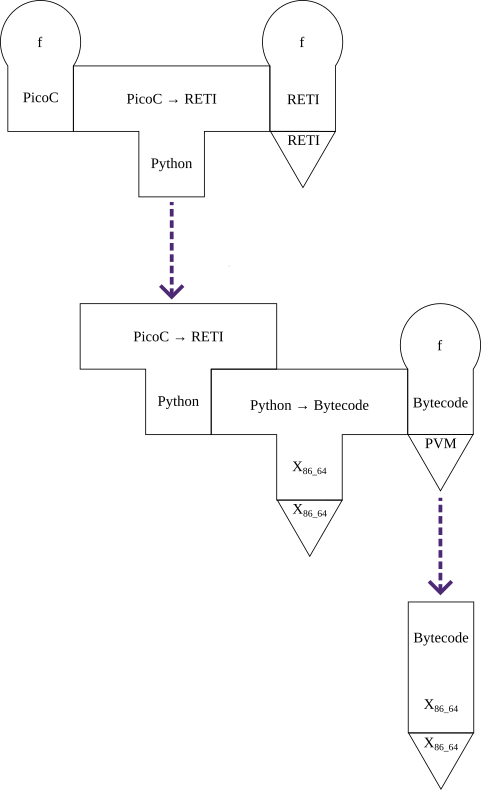
\includegraphics[width=0.5\linewidth]{./figures/summarized_cross_compiler.png}
  \caption{Cross-Compiler Kompiliervorgang ausgeschrieben}
  \label{fig:cross_compiler_kompiliervorgang_ausgeschrieben}
\end{figure}

Dieses längliche \colorbold{T-Diagram} in Abbildung~\ref{fig:cross_compiler_kompiliervorgang_ausgeschrieben} lässt sich zusammenfassen, sodass man das \colorbold{T-Diagram} in Abbildung~\ref{fig:cross_compiler_kompiliervorgang_kurzform} erhält, in welcher direkt angegeben ist, dass der \colorbold{PicoC-Compiler} in $\mathtt{X_{86\_64}}$-Maschienensprache geschrieben ist.

\begin{figure}[H]
  \centering
  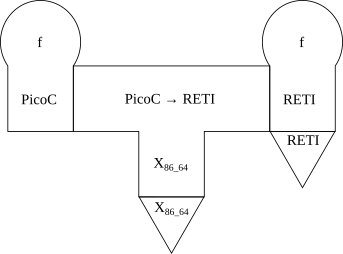
\includegraphics[width=0.33\linewidth]{./figures/compiliervorang_mit_machiene.png}
  \caption{Cross-Compiler Kompiliervorgang Kurzform}
  \label{fig:cross_compiler_kompiliervorgang_kurzform}
\end{figure}

Nachdem der Kompilierprozess des \colorbold{PicoC-Compiler} im \colorbold{vertikalen} nun genauer angesehen wurde, wird der Kompilierprozess im Folgenden im \colorbold{horinzontalen}, auf der Ebene der verschiedenen \colorbold{Passes} genauer betrachtet. Die Abbildung~\ref{fig:architektur_mit_allen_passes_ausgeschrieben} gibt einen guten Überblick über alle \colorbold{Passes} und wie diese in der \colorbold{Pipe-Architektur} (Definition~\ref{def:pipe_architektur}) des \colorbold{PicoC-Compilers} aufeinanderfolgen. In der \colorbold{Pipe-Architektur} nutzt der jeweils nächste \colorbold{Pass} den generierten \colorbold{Abstract Syntax Tree} des vorherigen Passes oder der Syntaktischen Analyse, um einen eigenen \colorbold{Abstract Syntax Tree} in seiner eigenen \colorbold{Sprache} zu generieren.

\begin{figure}[H]
  \centering
  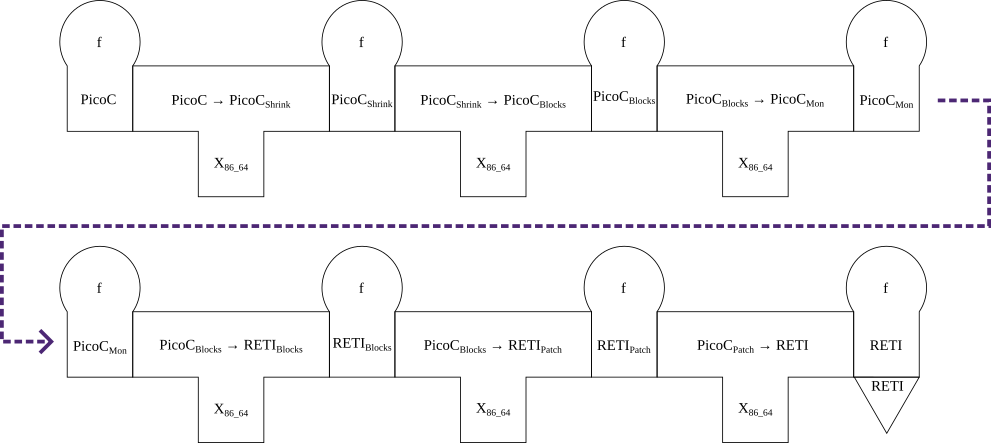
\includegraphics[width=\linewidth]{./figures/passes.png}
  \caption{Architektur mit allen Passes ausgeschrieben}
  \label{fig:architektur_mit_allen_passes_ausgeschrieben}
\end{figure}

Im Unterkapitel~\ref{sec:passes} werden die unterschiedlichen \colorbold{Passes} des PicoC-Compilers erklärt. In den darauffolgenden Unterkapiteln~\ref{sec:umsetzung_von_pointern},~\ref{sec:umsetzung_von_arrays},~\ref{sec:umsetzung_von_structs}~und~\ref{sec:umsetzung_von_funktionen} zu \colorbold{Pointern},  \colorbold{Arrays}, \colorbold{Structs} und \colorbold{Funktionen} werden einzelne \colorbold{Aspekte}, die Thema dieser \colorbold{Bachelorarbeit} sind \colorbold{genauer betrachtet} und erklärt, die im Unterkapitel~\ref{sec:passes} nicht ausreichend vertieft wurden. Viele der verwendenten \colorbold{Ansätze} zur Lösung dieser Probleme basieren auf der Vorlesung~\cite{scholl_betriebssysteme_2020} und wurden in dieser Bachelorarbeit weiter ausgearbeitet, wo es nötig war, sodass diese mit dem \colorbold{PicoC-Compiler} auch in der \colorbold{Praxis} implementiert werden konnten.

% https://tex.stackexchange.com/questions/167380/how-to-refer-to-a-footnote
Um die verschiedenen Aspekte besser erklären zu können, werden \colorbold{Codebeispiele} verwendet, in welchen ein kleines repräsentatives \colorbold{PicoC-Programm} für einen spezifischen Aspekt in wichtigen \colorbold{Zwischenstadien der Kompilierung} gezeigt wird\footnote{Also die verschiedenen in den \colorbold{Passes} generierten \colorbold{Abstract Syntax Trees}, sofern der \colorbold{Pass} für den gezeigten Aspekt relevant ist.}. Die \colorbold{Codebeispiele} wurden alle mit dem \colorbold{PicoC-Compiler} kompiliert und danach \colorbold{nicht} mehr \colorbold{verändert}, also genauso, wie der \colorbold{PicoC-Compiler} sie kompiliert aus den Dateien in dieses Dokument eingelesen. Alle hier zur Repräsentation verwendeten \colorbold{PicoC-Programme} lassen sich unter dem \footnoteurl{https://github.com/matthejue/Bachelorarbeit/tree/master/code_examples} finden und mithilfe der im Ordner \inlinebox{/code_examples} beiliegenden \inlinebox{Makefile} und dem Befehl \inlinebox*{make compile-all} genauso \colorbold{kompilieren}, wie sie hier dargestellt sind\footnote{Es wurden zu diesem Zweck spezielle neue \colorbold{Command-line Optionen} erstellt, die bestimmte Kommentare \colorbold{herausfiltern} und manche Container-Knoten \colorbold{einzeilig} machen, damit die generierten \colorbold{Abstract Syntax Trees} in den verscchiedenen Zwischenstufen der Kompilierung \colorbold{nicht} zu langgestreckt und \colorbold{überfüllt} mit Kommentaren sind.}.

\subsection{Passes}
\label{sec:passes}

Im Folgenden werden die verschiedenen \colorbold{Passes} des \colorbold{PicoC-Compilers} für die Generierung von \colorbold{RETI-Code} besprochen. Viele dieser \colorbold{Passes} haben \colorbold{Aufgaben}, die eher unter die Themenbereiche des \colorbold{Bachelorprojekts} fallen. Allerdings ist das Verständnis der \colorbold{Passes} auch für das Verständnis der veschiedenen Aspekte\footnote{In kurz: \colorbold{Pointer}, \colorbold{Arrays}, \colorbold{Strcuts} und \colorbold{Funktionen}.} der \colorbold{Bachelorarbeit} wichtig.

Auf jedes Detail der einzelnen \colorbold{Passes} wird in diesem Unterkapitel allerdings nicht eingegangen, da diese einerseits in den Unterkapiteln~\ref{sec:umsetzung_von_pointern},~\ref{sec:umsetzung_von_arrays},~\ref{sec:umsetzung_von_structs}~und~\ref{sec:umsetzung_von_funktionen} zu \colorbold{Pointern},  \colorbold{Arrays}, \colorbold{Structs} und \colorbold{Funktionen} im Detail erklärt sind und andererseits viele Aufgaben dieser \colorbold{Passes} eher dem \colorbold{Bachelorprojekt} zuzurechnen sind.

\subsubsection{PicoC-Shrink Pass}
\label{picoc_shrink_pass}
\newlineparagraph{Aufgabe}
\label{sec:picoc_shrink_pass_zweck}
% dieser Pass existiert nur wegen der Erweiterungen

Der Aufgabe des \colorbold{PicoC-Shrink Pass} ist in Unterkapitel~\ref{dereferenzierung_durch_zugriff_auf_arrayindex_ersetzen} ausführlich an einem Beispiel erklärt. Kurzgefasst hat der \colorbold{PicoC-Shrink Pass} die Aufgabe, die Eigenheit auszunutzen, dass der \colorbold{Dereferenzierungoperator} \smalltt{*pntr} und die damit einhergehende \colorbold{Pointer Arithmetik} \smalltt{*(pntr + i)} sich in der Untermenge der Sprache $L_{C}$, welche die Sprache $L_{PicoC}$ darstellt genau gleich verhält, wie der \colorbold{Operator} für den \colorbold{Zugriff} auf den \colorbold{Index} eines \colorbold{Arrays} \smalltt{ar[i]}.

Daher wandelt der \colorbold{PicoC-Shrink Pass} alle Verwendungen des \colorbold{Knoten} \smalltt{Deref(exp, i)} im jeweiligen \colorbold{Abstract Syntax Tree} in \colorbold{Knoten} \smalltt{Subscr(exp, i)} um, sodass sich dadurch viele vermeidbare \colorbold{Fallunterscheidungen} und \colorbold{doppelter Code} bei der Implementierung vermeiden lassen. Man lässt die  \colorbold{Derefenzierung} \smalltt{*(var + i)} einfach von den Routinen für einen \colorbold{Zugriff auf einen Arrayindex} \smalltt{var[i]} übernehmen.

\newlineparagraph{Abstrakte Syntax}

Die \colorbold{Abstrakte Syntax} der Sprache $L_{PicoC\_Shrink}$ in Tabelle~\ref{gr:abstract_syntax_l_picoc_shrink} ist fast \colorbold{identisch} mit der \colorbold{Abstrakten Syntax} der Sprache $L_{PiocC}$ in Tabelle~\ref{gr:abstract_syntax_l_picoc}, nach welcher der \colorbold{erste} Abstract Syntax Tree in der \colorbold{Syntaktischen Analyse} generiert wurde. Der einzige \colorbold{Unterschied} liegt darin, dass es den Knoten \smalltt{Deref(exp, exp)} in Tabelle~\ref{gr:abstract_syntax_l_picoc_shrink} \colorbold{nicht} mehr gibt. Das liegt daran, dass dieser Pass alle \colorbold{Vorkommnisse} des Knoten \smalltt{Deref(exp, exp)} durch den Knoten \smalltt{Subscr(exp, exp)} auswechselt, der ebenfalls bereits in der \colorbold{Abstrakten Syntax} der Sprache $L_{PicoC}$ definiert ist.

\begin{grammar}[Abstrakte Syntax der Sprache $L_{PiocC\_Shrink}$][H][gr:abstract_syntax_l_picoc_shrink]
  \toprule
  \commentsecond*
  \midrule
  \arith*
  \midrule
  \logic*
  \midrule
  \assign*
  \midrule
  \pntrshrink*
  \midrule
  \arraysecond*
  \midrule
  \struct*
  \midrule
  \ifelse*
  \midrule
  \loopsecond*
  \midrule
  \fun*
  \midrule
  \file*
  \bottomrule
\end{grammar}

\begin{Special_Paragraph}
  Der \textcolor{red}{rot} markierte Knoten bedeutet, dass dieser im Vergleich zur voherigen \colorbold{Abstrakten Syntax} nicht mehr da ist.
\end{Special_Paragraph}

\newlineparagraph{Codebeispiel}

In den nächsten Unterkapiteln wird das Beispiel in Code~\ref{code:picoc_code_für_codebeispiel} zur \colorbold{Anschauung} der verschiedenen \colorbold{Passes} verwendet. Im Code~\ref{code:picoc_code_für_codebeispiel} ist in der Funktion \smalltt{faculty} ein \colorbold{iterativer} Algorithmus implementiert, der die \colorbold{Fakultät} eines übergebenen \colorbold{Arguments} berechnet. Der Algorithmus basiert auf einem \colorbold{Beispielprogramm} aus der Vorlesung~\cite{scholl_betriebssysteme_2020}, welcher in der Vorlesung allerdings \colorbold{rekursiv} implementiert ist.
% natürlich beide Beispiele als Tests verfügbar

Dieser \colorbold{rekursive} Algoirthmus ist allerdings \colorbold{kein} gutes \colorbold{Anschaungsbeispiel}, dass viele der Aufgaben der verschiedenen \colorbold{Passes} bei der Kompilierung veranschaulicht hätte. Viele Aufgaben der \colorbold{Passes}, wie z.B. bei der Kompilierung von \smalltt{if}-, \smalltt{if-else}-, \smalltt{while}- und \smalltt{do-while}-Statements wären im Beispiel aus der Vorlesung \colorbold{nicht} enthalten gewesen. Daher wurde das Beispiel aus der Vorlesung zu einem \colorbold{iterativen} Algorithmus~\ref{code:picoc_code_für_codebeispiel} umgeschrieben, um \smalltt{if}- und \smalltt{while}-Statemtens zu enthalten.

Beide Varianten des \colorbold{Algorithmus} wurden zum \colorbold{Testen} des PicoC-Compilers verwendet und sind als Tests im Ordner \inlinebox{/tests} unter \footnoteurl{https://github.com/matthejue/PicoC-Compiler/tree/new_architecture/tests}, unter den Testbezeichnungen \inlinebox{example_faculty_rec.picoc} und \inlinebox{example_faculty_it.picoc} zu finden.

Die Codebeispiele in diesem und den folgenden Unterkapiteln dienen allerdings nur als \colorbold{Anschauung} des jeweiligen \colorbold{Passes}, der in diesem Unterkapitel beschrieben wird und werden nicht im Detail erläutert, da viele Details der Passes später in den Unterkapiteln~\ref{sec:umsetzung_von_pointern},~\ref{sec:umsetzung_von_arrays},~\ref{sec:umsetzung_von_structs}~und~\ref{sec:umsetzung_von_funktionen} zu \colorbold{Pointern},  \colorbold{Arrays}, \colorbold{Structs} und \colorbold{Funktionen} mit eigenen \colorbold{Codebeispielen} erklärt werden und alle sonstigen Details dem \colorbold{Bachelorprojekt} zuzurechnen sind.

\begin{code}
  \centering
  \numberedcodebox[minted language=c]{./code_examples/example_faculty_it.picoc}
  \caption{PicoC Code für Codebespiel}
  \label{code:picoc_code_für_codebeispiel}
\end{code}

In Code~\ref{code:abstract_syntax_tree_für_codebeispiel} sieht man den \colorbold{Abstract Syntax Tree}, der in der \colorbold{Syntaktischen Analyse} generiert wurde.

\begin{code}
  \centering
  \numberedcodebox[minted language=text]{./code_examples/example_faculty_it.ast}
  \caption{Abstract Syntax Tree für Codebespiel}
  \label{code:abstract_syntax_tree_für_codebeispiel}
\end{code}

Im \colorbold{PicoC-Shrink-Pass} ändert sich nichts im Vergleich zum \colorbold{Abstract Syntax Tree} in Code~\ref{code:abstract_syntax_tree_für_codebeispiel}, da das Codebeispiel keine \colorbold{Dereferenzierung} enthält.

% TODO: nichts hinzugefügt zu Syntax

\subsubsection{PicoC-Blocks Pass}
\label{picoc_blocks_pass}
\newlineparagraph{Aufgabe}
\label{sec:picoc_blocks_pass_zweck}

Die Aufgabe des \colorbold{PicoC-Blocks Passes} ist es die Knoten \smalltt{If(exp, stmts)}, \smalltt{IfElse(exp, stmts1, stmts2)}, \smalltt{While(exp, stmts)} und \smalltt{DoWhile(exp, stmts)} mithilfe von \smalltt{Block(name, stmts\_instrs}-, \smalltt{GoTo(lable)}- und \smalltt{IfElse(exp, stmts1, stmts2)}-Knoten umzusetzen. Der \smalltt{IfElse(exp, stmts1, stmts2)}-Knoten wird zur Umsetzung der \colorbold{Bedingung} verwendet und es wird, je nachdem, ob die Bedingung \colorbold{wahr} oder \colorbold{falsch} ist mithilfe der \smalltt{GoTo(label)}-Knoten in einen von zwei \colorbold{alternativen Branches} gesprungen oder ein \colorbold{Branch} erneut aufgerufen usw.

\newlineparagraph{Abstrakte Syntax}

Zur Umsetzung dieses Passes ist es notwendig die \colorbold{Abstrakte Syntax} der Sprache $L_{PicoC\_Shrink}$ in Tabelle~\ref{gr:abstract_syntax_l_picoc_shrink} um die Knoten zu erweitern, die im Unterkapitel \ref{sec:picoc_blocks_pass_zweck} erwähnt wurden. Die Knoten \smalltt{If(exp, stmts)}, \smalltt{While(exp, stmts)} und \smalltt{DoWhile(exp, stmts)} gibt es nicht mehr, da sie durch \smalltt{Block(name, stmts\_instrs}-, \smalltt{GoTo(lable)}- und \smalltt{IfElse(exp, stmts1, stmts2)}-Knoten ersetzt wurden. Die \colorbold{Funktionsdefinition} \smalltt{FunDef(⟨datatype⟩, Name(str), Alloc(Writeable(), ⟨datatype⟩, Name(str))*, ⟨block⟩*)} ist nun ein Container für \colorbold{Blöcke} \smalltt{Block(Name(str), ⟨stmt⟩*)} und keine Statements \smalltt{stmt} mehr. Das resultiert in der \colorbold{Abstrakten Syntax} der Sprache $L_{PicoC\_Blocks}$ in Tabelle~\ref{gr:abstract_syntax_l_picoc_blocks}.

\begin{grammar}[Abstrakte Syntax der Sprache $L_{PiocC\_Blocks}$][H][gr:abstract_syntax_l_picoc_blocks]
  \toprule
  \commentsecond*
  \midrule
  \arith*
  \midrule
  \logic*
  \midrule
  \assign*
  \midrule
  \pntrshrinkafter*
  \midrule
  \arraysecond*
  \midrule
  \struct*
  \midrule
  \ifelseblocks*
  \midrule
  \loopblocks*
  \midrule
  \funafter*
  \midrule
  \block
  \midrule
  \file*
  \bottomrule
\end{grammar}

\begin{Special_Paragraph}
  Alles \textcolor{red}{rot} markierte bedeutet, es wurde \colorbold{entfernt} oder \colorbold{abgeändert}. Alles \textcolor{gray!90!black}{ausgegraute} bedeutet, es hat sich im Vergleich zur letzten Abstrakten Syntax \colorbold{nichts} geändert. Alle normal in \smalltt{schwarz} geschriebenen Knoten wurden \colorbold{neu} hinzugefügt.

  Die \colorbold{Abstrakte Syntax} soll im Gegensatz zur \colorbold{Konkretten Syntax} meist nur vom \colorbold{Programmierer} verstanden werden und sollte daher vor allem \colorbold{einfach verständlich} sein und stellt daher eine \colorbold{Obermenge} aller tatsächlich möglichen \colorbold{Kompositionen} von \colorbold{Knoten} dar\footnote{D.h. auch wenn dort \smalltt{exp} als \colorbold{Attribut} steht, kann dort \colorbold{nicht} jeder Knoten, der sich aus der \colorbold{Produktion} \smalltt{exp} ergibt auch wirklich eingesetzt werden.}.

  Man bezeichnet hier die \colorbold{Abstrakte Syntax} als \colorbold{\enquote{Abstrakte Syntax der Sprache $L_{Picoc\_Blocks}$}}. Diese Sprache $L_{Picoc\_Blocks}$ wird durch eine \colorbold{Konkrette Syntax} beschrieben, die allerdings nicht weiter relevant ist, da in den \colorbold{Passes} nur \colorbold{Abstract Syntax Trees} umgeformt werden. Es ist hierbei nur wichtig zu wissen, dass die \colorbold{Abstrakte Syntax} theoretisch zur Kompilierung der Sprache $L_{Picoc\_Blocks}$ definiert ist, also die Sprache $L_{PicoC\_Blocks}$ nicht die Sprache ist, die von der \colorbold{Abstrakten Syntax} beschrieben ist.
\end{Special_Paragraph}
% TODO: man tut so als gäbe es Konkrette Syntax

\newlineparagraph{Codebeispiel}

In Code~\ref{code:picoc_blocks_pass_für_codebeispiel} sieht man den \colorbold{Abstract-Syntax-Tree} des \colorbold{PiocC-Blocks Passes} für das aus Unterkapitel~\ref{code:picoc_code_für_codebeispiel} weitergeführte Beispiel, indem nun eigene \colorbold{Blöcke} für die Funktion \smalltt{faculty} und die \smalltt{main}-Funktion erstellt werden, in denen die \colorbold{ersten} Statements der jeweiligen Funktionen bis zum \colorbold{letzten} Statement oder bis zum ersten \colorbold{Auftauchen} eines \smalltt{If(exp, stmts)}-, \smalltt{IfElse(exp, stmts1, stmts2)}-, \smalltt{While(exp, stmts)}- oder \smalltt{DoWhile(exp, stmts)}-Knoten stehen. Je nachdem, ob ein \smalltt{If(exp, stmts)}-, \smalltt{IfElse(exp, stmts1, stmts2)}-, \smalltt{While(exp, stmts)}- oder \smalltt{DoWhile(exp, stmts)}-Knoten auftaucht, werden für die \colorbold{Bedingung} und mögliche \colorbold{Branches} eigene \colorbold{Blöcke} erstellt.

\begin{code}
  \centering
  \numberedcodebox[minted language=text]{./code_examples/example_faculty_it.picoc_blocks}
  \caption{PicoC-Blocks Pass für Codebespiel}
  \label{code:picoc_blocks_pass_für_codebeispiel}
\end{code}

\subsubsection{PicoC-ANF Pass}
\label{picoc_mon_pass}

\newlineparagraph{Aufgabe}
\label{sec:picoc_mon_pass_zweck}

Die Aufgabe des \colorbold{PicoC-ANF Passes} ist es den \colorbold{Abstract Syntax Tree} der Sprache $L_{PicoC\_Blocks}$ in die \colorbold{Abstrakte Syntax} der Sprache $L_{PicoC\_ANF}$ umzuformen, welche in \colorbold{A-Normalform} (Definition~\ref{def:a_normal_form}) und damit auch in \colorbold{Monadischer Normalform} (Definition~\ref{def:monadische_normalform}) ist. Um Wiederholung zu vermeiden wird zur Erklärung der \colorbold{A-Normalform} auf Unterkapitel~\ref{sec:a_normalform} verwiesen.

Zudem wird eine \colorbold{Symboltabelle} (Definition~\ref{def:symboltabelle}) eingeführt. In der \colorbold{Symboltabelle} wird beim Anlegen eines \colorbold{neuen Eintrags} für eine Variable zunächst eine \colorbold{Adresse} zugewiesen, die dem Wert einer von zwei \colorbold{Countern}  \smalltt{rel\_global\_addr} und  \smalltt{rel\_stack\_addr} entspricht. Der Counter \smalltt{rel\_global\_addr} ist für Variablen in den \colorbold{Globalen Statischen Daten} und der \colorbold{Counter}  \smalltt{rel\_stack\_addr} ist für Variablen auf dem \colorbold{Stackframe}. Einer der beiden \colorbold{Counter} wird entsprechend der \colorbold{Größe} der angelegten Variable \colorbold{hochgezählt}.

Kommt im \colorbold{Programmcode} an einer späteren Stelle diese Variable \smalltt{Name('symbol')} vor, so wird mit dem \colorbold{Symbol}\footnote{Bzw. der \colorbold{Bezeichner}} als Schlüssel in der \colorbold{Symboltabelle} nachgeschlagen und anstelle des \smalltt{Name(str)}-Knotens die in der \colorbold{Symboltabelle} nachgeschlagene Adresse in einem \smalltt{Global(Num('addr'))}- bzw. \smalltt{Stackframe(Num('addr'))}-Knoten eingesetzt eingefügt. Ob der \smalltt{Global(Num('addr'))}- oder  der \smalltt{Stackframe(Num('addr'))}-Knoten zum Einsatz kommt, entscheidet sich anhand des \colorbold{Scopes} (z.B. \smalltt{@scope}), der in der \colorbold{Symboltabelle} an den \colorbold{Bezeichner} drangehängt ist (z.B. \smalltt{identifier@scope}).\footnote{Die Umsetzung von \colorbold{Scopes} wird in Unterkapitel~\ref{sec:funktionsdeklaration_und_definition_und_umsetzung_von_scopes} genauer beschrieben.}

\begin{Definition}{Symboltabelle}{symboltabelle}
  Eine über ein \colorbold{Assoziatives Feld} umgesetzte \colorbold{Datenstruktur}, die notwendig ist, um das Konzept einer \colorbold{Variablen} in einer Sprache umzusetzen. Diese Datenstruktur ordnet jedem \colorbold{Symbol}\footnote{In einer \colorbold{Symboltabelle} werden \colorbold{Bezeichner} als \colorbold{Symbole} bezeichnet.} einer \colorbold{Variablen}, \colorbold{Konstanten} oder \colorbold{Funktion} aus einem \colorbold{Programm}, Informationen, wie die \colorbold{Adresse}, die \colorbold{Position} im Programmcode oder den \colorbold{Datentyp} zu.

  Die \colorbold{Symboltabelle} muss nur während des \colorbold{Kompiliervorgangs} im \colorbold{Speicher} existieren, da die Einträge in der \colorbold{Symboltabelle} beeinflussen, was für \colorbold{Maschinencode} generiert wird und dadurch im \colorbold{Maschinencode} bereits die richtigen \colorbold{Adressen} usw. angesprochen werden und es die Symboltabelle selbst \colorbold{nicht} mehr braucht.
\end{Definition}

\newlineparagraph{Abstrakte Syntax}

Zur Umsetzung dieses Passes ist es notwendig die \colorbold{Abstrakte Syntax} der Sprache $L_{PicoC\_Blocks}$ in Tabelle~\ref{gr:abstract_syntax_l_picoc_blocks} in die \colorbold{A-Normalform} zu bringen. Darunter fällt es unter anderem, dafür zu sorgen, dass \colorbold{Komplexe Knoten}, wie z.B. \smalltt{BinOp(exp, bin\_op, exp)} nur \colorbold{Atomare Knoten}, wie z.B. \smalltt{Stack(Num(str))} enthalten können. Des Weiteren werden auch \colorbold{Funktionen} und \colorbold{Funktionsaufrufe} aufgelöst, sodass u.a. die \colorbold{Blöcke} \smalltt{Block(Name(str), stmt*)} nun direkt im \smalltt{File(Name(str), block*)}-Knoten liegen usw., was in Unterkapitel~\ref{sec:umsetzung_von_funktionen} genauer erklärt wird. Die \colorbold{Symboltabelle} ist ebenfalls als \colorbold{Abstract Syntax Tree} umgesetzt, wofür in der \colorbold{Abstrakten Syntax} der Sprache $L_{PicoC\_ANF}$ in Grammatik~\ref{gr:abstract_syntax_l_picoc_anf} neue Knoten eingeführt werden.

Das ganze resultiert in der \colorbold{Abstrakten Syntax} der Sprache $L_{PicoC\_ANF}$ in Grammatik~\ref{gr:abstract_syntax_l_picoc_anf}.

\begin{grammar}[Abstrakte Syntax der Sprache $L_{PiocC\_ANF}$][H][gr:abstract_syntax_l_picoc_anf]
  \toprule
  \commentsecond*
  \midrule
  \arithanf
  \midrule
  \logicanf
  \midrule
  \assignanf
  \midrule
  \pntranf*
  \midrule
  \arrayanf*
  \midrule
  \struct*
  \midrule
  \ifelseanf*
  \midrule
  \funanf*
  \midrule
  \block*
  \midrule
  \fileanf*
  \midrule
  \symbolsecond
  \bottomrule
\end{grammar}

\newlineparagraph{Codebeispiel}

In Code~\ref{code:picoc_mon_pass_für_codebeispiel} sieht man den \colorbold{Abstract-Syntax-Tree} des \colorbold{PiocC-ANF Passes} für das aus Unterkapitel~\ref{code:picoc_code_für_codebeispiel} weitergeführte Beispiel, indem alls Statements und Ausdrücke in \colorbold{A-Normalform} sind. Die \smalltt{IfElse(exp, stmts, stmts)}-Knoten sind hier in  \colorbold{A-Normalform} gebracht worden, indem ihre \colorbold{Komplexe Bedingung} vorgezogen wurde und das Ergebnis der \colorbold{Komplexen Bedingung} einer \colorbold{Location} zugewiesen ist und sie selbst das Ergebnis über den \colorbold{Atomaren Ausdruck} \smalltt{Stack(Num(str))} vom Stack lesen: \smalltt{IfElse(Stack(Num(str)), stmts, stmts)}. \colorbold{Funktionen} sind nur noch über die \colorbold{Labels} von Blöcken zu erkennen, die den gleichen Bezeichner haben, wie die ursprüngliche Funktion und es lässt sich nur durch das \colorbold{Nachverfolgen} der \smalltt{GoTo(Name('label'))}-Knoten nachvollziehen, was ursprünglich zur Funktion gehörte.

\begin{code}
  \centering
  \numberedcodebox[minted language=text]{./code_examples/example_faculty_it.picoc_mon}
  \caption{PicoC-ANF Pass für Codebespiel}
  \label{code:picoc_mon_pass_für_codebeispiel}
\end{code}

\subsubsection{RETI-Blocks Pass}
\label{reti_blocks_pass}

\newlineparagraph{Aufgaben}
\label{sec:reti_blocks_pass_zweck}

Die Aufgabe des \colorbold{RETI-Blocks Passes} ist es die \colorbold{Statements} in der \colorbold{Blöcken}, die durch \colorbold{PicoC-Knoten} im \colorbold{Abstract Syntax Tree} der Sprache $L_{PicoC\_ANF}$ dargestellt sind durch ihren entsprechenden \colorbold{RETI-Knoten} zu ersetzen.

\newlineparagraph{Abstrakte Syntax}

Die \colorbold{Abstrakte Syntax} der Sprache $L_{RETI\_Blocks}$ in Grammatik~\ref{gr:abstract_syntax_l_reti_blocks} ist verglichen mit der \colorbold{Abstrakten Syntax} der Sprache $L_{PicoC\_ANF}$ in Grammatik~\ref{gr:abstract_syntax_l_picoc_anf} stark verändert, denn der Großteil der \colorbold{PicoC-Knoten} wird in diesem Pass durch entsprechende \colorbold{RETI-Knoten} ersetzt. Die einzigen verbleibenden \colorbold{PicoC-Knoten} sind \smalltt{Exp(GoTo(str))}, \smalltt{Block(Name(str), ⟨instr⟩*)} und \smalltt{File(Name(str), ⟨block⟩*)}, da das gesamte Konzept mit den \colorbold{Blöcken} erst im \colorbold{RETI-Pass} in Unterkapitel~\ref{gr:abstract_syntax_l_reti} aufgelöst wird.

\begin{grammar}[Abstrakte Syntax der Sprache $L_{RETI\_Blocks}$][H][gr:abstract_syntax_l_reti_blocks]
  \toprule
  \retiblocks
  \midrule
  \picocblocksleftover
  \bottomrule
\end{grammar}

\newlineparagraph{Codebeispiel}

In Code~\ref{code:reti_blocks_pass_für_codebeispiel} sieht man den \colorbold{Abstract-Syntax-Tree} des \colorbold{RETI-Blocks Passes} für das aus Unterkapitel~\ref{code:picoc_code_für_codebeispiel} weitergeführte Beispiel, indem die \colorbold{Statements}, die durch entsprechende \colorbold{PicoC-Knoten} im \colorbold{Abstrakt Syntax Tree} der Sprache $L_{PicoC\_ANF}$ in Grammatik~\ref{gr:abstract_syntax_l_picoc_anf} repräsentiert waren nun durch ihre entsprechennden \colorbold{RETI-Knoten} ersetzt werden.

\begin{code}
  \centering
  \numberedcodebox[minted language=text]{./code_examples/example_faculty_it.reti_blocks}
  \caption{RETI-Blocks Pass für Codebespiel}
  \label{code:reti_blocks_pass_für_codebeispiel}
\end{code}

\begin{Special_Paragraph}
  Theoretisch ist das kein richtiger \colorbold{Abstrakt Syntax Tree} mehr, da die die \colorbold{RETI-Knoten} in \colorbold{Konkretter Syntax} sind und nicht in \colorbold{Abstrakter Syntax}.
\end{Special_Paragraph}

\subsubsection{RETI-Patch Pass}
\label{reti_patch_pass}

\newlineparagraph{Aufgaben}
\label{sec:reti_patch_pass_zweck}

\newlineparagraph{Abstrakte Syntax}

\begin{grammar}[Abstrakte Syntax der Sprache $L_{RETI\_Patch}$][H][gr:abstract_syntax_l_reti_patch]
  \toprule
  \retiblocks*
  \midrule
  \picocblocksleftover*
  \bottomrule
\end{grammar}

\newlineparagraph{Codebeispiel}

% In Code~\ref{code:} sieht man den \colorbold{Abstract-Syntax-Tree} des \colorbold{PiocC-ANF Passes} für das aus Unterkapitel~\ref{code:} weitergeführte Beispiel, indem

\begin{code}
  \centering
  \numberedcodebox[minted language=text]{./code_examples/example_faculty_it.reti_patch}
  \caption{RETI-Patch Pass für Codebespiel}
  \label{code:reti_patch_pass_für_codebeispiel}
\end{code}

\subsubsection{RETI Pass}
\label{reti_pass}

\newlineparagraph{Aufgaben}
\label{sec:reti_pass_zweck}

\newlineparagraph{Konkrette und Abstrakte Syntax}

% dieser Pass entspricht Assembler bis auf die Sache mit binärer Repräsentation, was der PicoC-Compiler garnicht macht

\begin{grammar}[Konkrette Syntax der Sprache $L_{RETI\_Lex}$][H][gr:konkrette_syntax_l_reti_lexer]
  \toprule
  \firstcase{dig\_no\_0}{ \dq 1\dq \gralt \dq 2\dq \gralt \dq 3\dq \gralt \dq 4\dq \gralt \dq 5\dq \gralt \dq 6\dq}{L\_Program}
  \otherform{\dq 7\dq \gralt \dq 8\dq \gralt \dq 9\dq}{}
  \firstcase{dig\_with\_0}{ \dq 0\dq \gralt dig\_no\_0}{}
  \firstcase{num}{ \dq 0\dq \gralt dig\_no\_0 \enspace dig\_with\_0*\gralt \dq {-}\dq dig\_no\_0*}{}
  \firstcase{letter}{ \dq a\dq ... \dq Z\dq }{}
  \firstcase{name}{ letter(letter \mid  dig\_with\_0 \mid  \_)*}{}
  \firstcase{reg}{ \dq ACC\dq \gralt \dq IN1\dq \gralt \dq IN2\dq \gralt \dq PC\dq \gralt \dq SP\dq}{}
  \otherform{\dq BAF\dq \gralt \dq CS\dq \gralt \dq DS\dq}{}
  \firstcase{arg}{ reg \gralt  num}{}
  \firstcase{rel}{ \dq {==}\dq \gralt \dq {!=}\dq \gralt \dq {<}\dq \gralt \dq {<=}\dq\gralt \dq {>}\dq}{}
  \otherform{\dq {>=}\dq \gralt \dq \_NOP\dq}{}
  \bottomrule
\end{grammar}

\begin{grammar}[Konkrette Syntax der Sprache $L_{RETI\_Parse}$][H][gr:konkrette_syntax_l_reti_parser]
\toprule
\firstcase{instr}{\dq ADD\dq\enspace reg\enspace arg\gralt \dq ADDI\dq\enspace reg\enspace num\gralt \dq SUB\dq\enspace reg\enspace arg}{L\_Program}
\otherform{\dq SUBI\dq\enspace reg\enspace\enspace num\gralt \dq MULT\dq\enspace reg\enspace arg\gralt \dq MULTI\dq\enspace reg\enspace num}{}
\otherform{\dq DIV\dq\enspace reg\enspace arg\gralt \dq DIVI\dq\enspace reg\enspace num\gralt \dq MOD\dq\enspace reg\enspace arg}{}
\otherform{\dq MODI\dq\enspace reg\enspace num\gralt \dq OPLUS\dq\enspace reg\enspace arg\gralt \dq OPLUSI\dq\enspace reg\enspace num}{}
\otherform{\dq OR\dq\enspace reg\enspace arg\gralt \dq ORI\dq\enspace reg\enspace num}{}
\otherform{\dq AND\dq\enspace reg\enspace arg\gralt \dq ANDI\dq\enspace reg\enspace num}{}
\otherform{\dq LOAD\dq\enspace reg\enspace num\gralt \dq LOADIN\dq\enspace arg\enspace arg\enspace num}{}
\otherform{\dq LOADI\dq\enspace reg\enspace num}{}
\otherform{\dq STORE\dq\enspace reg\enspace num\gralt \dq STOREIN\dq\enspace arg\enspace arg num}{}
\otherform{\dq MOVE\dq\enspace reg\enspace reg}{}
\otherform{\dq JUMP\dq rel\enspace num\gralt INT\enspace num\gralt RTI}{}
\otherform{\dq CALL\dq\enspace \dq INPUT\dq\enspace  reg\gralt \dq CALL\dq\enspace \dq PRINT\dq\enspace reg}{}
\firstcase{program}{name\enspace (instr\dq ;\dq )*}{}
\bottomrule
\end{grammar}

% TODO: es braucht noch eine Konkrette Syntax dafür
\begin{grammar}[Abstrakte Syntax der Sprache $L_{RETI}$][H][gr:abstract_syntax_l_reti]
  \toprule
  \reti
  \midrule
  \picocremovedleftover
  \bottomrule
\end{grammar}

\newlineparagraph{Codebeispiel}

\begin{code}
  \centering
  \numberedcodebox[minted language=text]{./code_examples/example_faculty_it.reti}
  \caption{RETI Pass für Codebespiel}
  \label{code:reti_pass_für_codebeispiel}
\end{code}

% TODO: zusammenfassendes Bild
  % ./content/Implementierung1_Tables_DT_AST.tex
  %!Tex Root = ../Main.tex
% ./Packete_und_Deklarationen.tex
% ./Titlepage.tex
% ./Motivation.tex
% ./Einführung.tex
% ./Implementierung1_Tables_DT_AST.tex,
% ./Implementierung3_Struct_Derived.tex,
% ./Implementierung4_Fun.tex,
% ./Ergebnisse_und_Ausblick.tex

\subsection{Umsetzung von Pointern}
\subsubsection{Referenzierung}
Die \colorbold{Referenzierung} (z.B. \verb|&var|) wird im Folgenden anhand des Beispiels in Code~\ref{code:picoc_code_für_pointer_referenzierung} erklärt.

\begin{code}
  \centering
  \numberedcodebox[minted language=c, minted options={highlightlines={3}}]{./code_examples/example_pntr_ref.picoc}
  \caption{PicoC-Code für Pointer Referenzierung}
  \label{code:picoc_code_für_pointer_referenzierung}
\end{code}

Der Knoten \smalltt{Ref(Name('var')))} repräsentiert im \colorbold{Abstract Syntax Tree} in Code~\ref{code:abstract_syntax_tree_für_pointer_referenzierung} eine \colorbold{Referenzierung} \verb|&var| und der Knoten \smalltt{PntrDecl(Num('1'), IntType('int'))} repräsentiert einen Pointer \smalltt{*pntr}.

\begin{code}
  \centering
  \numberedcodebox[minted language=text, minted options={highlightlines={10}}]{./code_examples/example_pntr_ref.ast}
  \caption{Abstract Syntax Tree für Pointer Referenzierung}
  \label{code:abstract_syntax_tree_für_pointer_referenzierung}
\end{code}

Bevor man einem \colorbold{Pointer} eine eine \colorbold{Adresse} (z.B. \smalltt{\&var}) zuweisen kann, muss dieser erstmal \colorbold{definiert} sein. Dafür braucht es einen Eintrag in der \colorbold{Symboltabelle} in Code~\ref{code:symboltabelle_für_pointer_referenzierung}.

\begin{Special_Paragraph}
Die \colorbold{Größe} eines Pointers (z.B. eines Pointers auf ein Array von \smalltt{int}: \smalltt{pntr = int *pntr[3]}), die ihm \smalltt{size}-Feld der \colorbold{Symboltabelle} eingetragen ist, ist dabei immer: $\mathtt{size(pntr) = 1}$.
\end{Special_Paragraph}

\begin{code}
  \centering
  \numberedcodebox[minted language=text, minted options={highlightlines={23-28}}]{./code_examples/example_pntr_ref.st}
  \caption{Symboltabelle für Pointer Referenzierung}
  \label{code:symboltabelle_für_pointer_referenzierung}
\end{code}

Im \colorbold{PicoC-Mon Pass} in Code~\ref{code:picoc_mon_für_pointer_referenzierung} wird der Knoten \smalltt{Ref(Name('var')))} durch die Knoten \smalltt{Ref(GlobalRead(Num('0')))} und \smalltt{Assign(GlobalWrite(Num('1')), Tmp(Num('1')))} ersetzt. Im Fall, dass in \smalltt{Ref(exp))} das \smalltt{exp} vielleicht nicht direkt ein \smalltt{Name('var')} enthält und \smalltt{exp} z.B. ein \smalltt{Subscr(Attr(Name('var')))} ist, sind noch weitere Anweisungen zwischen den Zeilen \smalltt{11} und  \smalltt{12} nötig, die sich in diesem Beispiel um das Übersetzen von \smalltt{Subscr(exp)} und \smalltt{Attr(exp)} nach dem Schema in Subkapitel~\ref{sec:mittelteil_für_die_verschiedenen_derived_datatypes} kümmern.

\begin{code}
  \centering
  \numberedcodebox[minted language=text, minted options={highlightlines={11-12}}]{./code_examples/example_pntr_ref.picoc_mon}
  \caption{PicoC-Mon Pass für Pointer Referenzierung}
  \label{code:picoc_mon_für_pointer_referenzierung}
\end{code}

Im \colorbold{RETI-Blocks Pass} in Code~\ref{code:reti_blocks_für_pointer_referenzierung} werden die \colorbold{PicoC-Knoten} \smalltt{ Ref(Global(Num('0')))} und \smalltt{Assign(Global(Num('1')), Stack(Num('1')))} durch ihre entsprechenden \colorbold{RETI-Knoten} ersetzt.

\begin{code}
  \centering
  \numberedcodebox[minted language=text, minted options={highlightlines={18-21,23-25}}]{./code_examples/example_pntr_ref.reti_blocks}
  \caption{RETI-Blocks Pass für Pointer Referenzierung}
  \label{code:reti_blocks_für_pointer_referenzierung}
\end{code}
% Initialisierung eines Pointers
\subsubsection{Dereferenzierung durch Zugriff auf Arrayindex ersetzen}
Die \colorbold{Dereferenzierung} (z.B. \smalltt{*var}) wird im Folgenden anhand des Beispiels in Code~\ref{code:picoc_code_für_pointer_dereferenzierung} erklärt.

\begin{code}
  \centering
  \numberedcodebox[minted language=c, minted options={highlightlines={4}}]{./code_examples/example_pntr_deref.picoc}
  \caption{PicoC-Code für Pointer Dereferenzierung}
  \label{code:picoc_code_für_pointer_dereferenzierung}
\end{code}

Der Knoten \smalltt{Deref(Name('var')))} repräsentiert im \colorbold{Abstract Syntax Tree} in Code~\ref{code:abstract_syntax_tree_für_pointer_dereferenzierung} eine \colorbold{Dereferenzierung} \smalltt{*var}.

\begin{code}
  \centering
  \numberedcodebox[minted language=text, minted options={highlightlines={11}}]{./code_examples/example_pntr_deref.ast}
  \caption{Abstract Syntax Tree für Pointer Dereferenzierung}
  \label{code:abstract_syntax_tree_für_pointer_dereferenzierung}
\end{code}

Im \colorbold{PicoC-Shrink Pass} in Code~\ref{code:picoc_shrink_für_pointer_dereferenzierung} wird ein Trick angewandet, bei dem jeder Knoten \smalltt{Deref(Name('pntr'), Num('0'))} einfach durch den Knoten \smalltt{Subscr(Name('pntr'), Num('0'))} ersetzt wird. Der Trick besteht darin, dass der \colorbold{Dereferenzoperator} (z.B. \smalltt{*(var + 1)}) sich identisch zum \colorbold{Operator für den Zugriff auf einen Arrayindex} (z.B. \smalltt{var[1]}) verhält\footnote{In der Sprache $L_{C}$ gibt es einen Unterschied bei der Initialisierung bei z.B. \smalltt{int *var = \dq string\dq} und z.B. \smalltt{int var[1] = \dq string\dq}, der allerdings nichts mit den beiden Operatoren zu tuen hat, sondern mit der \colorbold{Initialisierung}, bei der die Sprache $L_{C}$ verwirrenderweise die eckigen Klammern \smalltt{[]} genauso, wie beim \colorbold{Operator für den Zugriff auf einen Arrayindex}, vor den Bezeichner schreibt (z.B. \smalltt{var[1]}), obwohl es ein \colorbold{Derived Datatype} ist.}. Damit sparrt man sich viele vermeidbare \colorbold{Fallunterscheidungen} und \colorbold{doppelten Code} und kann die \colorbold{Derefenzierung} (z.B. \smalltt{*(var + 1)}) einfach von den Routinen für einen \colorbold{Zugriff auf einen Arrayindex} (z.B. \smalltt{var[1]}) übernehmen lassen.

\begin{code}
  \centering
  \numberedcodebox[minted language=text, minted options={highlightlines={11}}]{./code_examples/example_pntr_deref.picoc_shrink}
  \caption{PicoC-Shrink Pass für Pointer Dereferenzierung}
  \label{code:picoc_shrink_für_pointer_dereferenzierung}
\end{code}

\subsection{Umsetzung von Arrays}
\subsubsection{Initialisierung von Arrays}
\label{sec:initialisierung_von_arrays}

Die \colorbold{Initialisierung} eines \colorbold{Arrays} (z.B. \smalltt{int ar[2][1] = \{\{3+1\}, \{4\}\}}) wird im Folgenden anhand des Beispiels in Code~\ref{code:picoc_code_für_array_initialisierung} erklärt.

% Stack und Globale Statische Daten
\begin{code}
  \centering
  \numberedcodebox[minted language=c, minted options={highlightlines={2, 6}}]{./code_examples/example_array_init.picoc}
  \caption{PicoC-Code für Array Initialisierung}
  \label{code:picoc_code_für_array_initialisierung}
\end{code}

Die \colorbold{Initialisierung} eines \colorbold{Arrays} \smalltt{int ar[2][1] = \{\{3+1\}, \{4\}\}} wird im \colorbold{Abstract Syntax Tree} in Code~\ref{code:abstract_syntax_tree_für_array_initialisierung} mithilfe der Komposition \smalltt{Assign(Alloc(Writeable(), ArrayDecl([Num('2'), Num('1')], IntType('int')), Name('ar')), Array([Array([BinOp(Num('3'), Add('+'), Num('1'))]), Array([Num('4')])]))} dargestellt.

\begin{code}
  \centering
  \numberedcodebox[minted language=text, minted options={highlightlines={9, 16}}]{./code_examples/example_array_init.ast}
  \caption{Abstract Syntax Tree für Array Initialisierung}
  \label{code:abstract_syntax_tree_für_array_initialisierung}
\end{code}

Bei der \colorbold{Initialisierung} eines \colorbold{Arrays} wird zuerst \smalltt{Alloc(Writeable(), ArrayDecl([Num('2'), Num('1')], IntType('int')))} ausgewertet, da eine Variable zuerst definiert sein muss, bevor man sie verwenden kann\footnote{Das Widerspricht der üblichen Auswertungsreihenfolge beim \colorbold{Zuweisungsoperator} \smalltt{=}, der \colorbold{rechtsassoziativ} ist. Der \colorbold{Zuweisungsoperator} \smalltt{=} tritt allerdings erst später in Aktion.}. Das \colorbold{Definieren} der Variable \smalltt{ar} erfolgt mittels der \colorbold{Symboltabelle}, die in Code~\ref{code:symboltabelle_für_array_initialisierung} dargestellt ist.

Bei Variablen auf dem \colorbold{Stackframe} wird ein Array \colorbold{rückwärts} auf das Stackframe geschrieben und auch die \colorbold{Adresse des ersten Elements} als Adresse des Arrays genommen. Dies macht den \colorbold{Zugriff auf einen Arrayindex} in Subkapitel~\ref{sec:zugriff_auf_arrayindex} deutlich unkomplizierter, da man so nicht mehr zwischen \colorbold{Stackframe} und \colorbold{Globalen Statischen Daten} beim \colorbold{Zugriff auf einen Arrayindex} unterscheiden muss, da es Probleme macht, dass ein \colorbold{Stackframe} in die entgegengesetzte Richtung wächst, verglichen mit den \colorbold{Globalen Statischen Daten}\footnote{Wenn man beim \colorbold{GCC}~\cite{noauthor_gcc_nodate} einen Stackframe mittels des \colorbold{GDB}~\cite{noauthor_gcc_nodate} beobachtet, sieht man, dass dieser es genauso macht.}.

\begin{Special_Paragraph}
  Das \colorbold{Größe} des Arrays $\mathtt{datatype \enspace ar[dim_1]\ldots[dim_k]}$, die ihm \smalltt{size}-Feld des \colorbold{Symboltabelleneintrags} eingetragen ist, berechnet sich dabei aus der \colorbold{Mächtigkeit} der einzelnen \colorbold{Dimensionen} des Arrays multipliziert mit der \colorbold{Größe} des \colorbold{grundlegenden Datentyps} der einzelnen \colorbold{Arrayelemente}: $\mathtt{size(datatype(ar)) = \left(\prod^n_{j=1} dim_j\right)\cdot size(datatype)}$\footnote{Die \colorbold{Funktion}  \smalltt{type} ordnet einer  \colorbold{Variable} ihren \colorbold{Datentyp} zu. Das ist notwendig, weil die \colorbold{Funktion} \smalltt{size} nur bei einem \colorbold{Datentyp} als \colorbold{Funktionsargument} die \colorbold{Größe dieses Datentyps} als \colorbold{Zielwert} liefert}.
\end{Special_Paragraph}

\begin{code}
  \centering
  \numberedcodebox[minted language=text, minted options={highlightlines={14-19,32-37}}]{./code_examples/example_array_init.st}
  \caption{Symboltabelle für Array Initialisierung}
  \label{code:symboltabelle_für_array_initialisierung}
\end{code}

Im \colorbold{PiocC-Mon Pass} in Code~\ref{code:picoc_mon_für_array_initialisierung} werden zuerst die \colorbold{Logischen Ausdrücke} in den Blättern des Teilbaums, der beim \colorbold{Array-Initializers} \colorbold{Container-Knoten} \smalltt{Array([Array([BinOp(Num('3'), Add('+'), Num('1'))]), Array([Num('4')])])} anfängt nach dem \colorbold{Depth-First-Search} Schema, von \colorbold{links-nach-rechts} ausgewertet und auf den \colorbold{Stack} geschrieben\footnote{Da der \colorbold{Zuweisungsoperator} \smalltt{=} \colorbold{rechtsassoziativ} ist und auch rein \colorbold{logisch}, weil man nichts zuweisen kann, was man noch nicht berechnet hat.}.

Im finalen Schritt muss zwischen \colorbold{Globalen Statischen Daten} bei der \smalltt{main}-Funktion und \colorbold{Stackframe} bei der Funktion \smalltt{fun} unterschieden werden. Die auf den Stack ausgewerteten Expressions werden mittels der Komposition \smalltt{Assign(Global(Num('0')), Stack(Num('2')))} bzw. \smalltt{Assign(Stackframe(Num('3')), Stack(Num('4')))}, die in Tabelle~\ref{tab:kompositionen_von_picoc_knoten_und_reti_knoten_mit_besonderer_bedeutung} genauer beschrieben ist, versetzt in der selben Reihenfolge zu den \colorbold{Globalen Statischen Daten} bzw. auf den \colorbold{Stackframe} geschrieben.

Der \colorbold{Trick} ist hier, dass egal wieviele Dimensionen und was für einen Datentyp das \colorbold{Array} hat, man letztendlich immer das gesamte Array erwischt, wenn man einfach die \colorbold{Größe des Arrays} viele \colorbold{Speicherzellen} mit z.B. der \colorbold{Komposition} \smalltt{Assign(Global(Num('0')), Stack(Num('2')))} verschiebt.

In die Knoten \smalltt{Global('0')} und  \smalltt{Stackframe('3')} wurde hierbei die \colorbold{Startadresse} des jeweiligen Arrays geschrieben, sodass man nach dem \colorbold{PicoC-Mon Pass} nie mehr Variablen in der  \colorbold{Symboltabelle} nachsehen muss und gleich weiß, ob sie in Bezug zu den \colorbold{Globalen Statischen Daten} oder dem \colorbold{Stackframe} stehen.

\begin{code}
  \centering
  \numberedcodebox[minted language=text, minted options={highlightlines={8-12,19-23}}]{./code_examples/example_array_init.picoc_mon}
  \caption{PicoC-Mon Pass für Array Initialisierung}
  \label{code:picoc_mon_für_array_initialisierung}
\end{code}

Im \colorbold{RETI-Blocks Pass} in Code~\ref{code:reti_blocks_für_array_initialisierung} werden die \colorbold{Kompositionen} \smalltt{Exp(exp)} und \smalltt{Assign(Global(Num('0')), Stack(Num('2')))} bzw. \smalltt{Assign(Stackframe(Num('3')), Stack(Num('4')))} durch ihre entsprechenden \colorbold{RETI-Knoten} ersetzt.

\begin{code}
  \centering
  \numberedcodebox[minted language=text, minted options={highlightlines={9-11,13-15,17-21,23-25,27-31,40-42,44-46,48-50,52-54,56-64}}]{./code_examples/example_array_init.reti_blocks}
  \caption{RETI-Blocks Pass für Array Initialisierung}
  \label{code:reti_blocks_für_array_initialisierung}
\end{code}


% kleines Extra
\subsubsection{Zugriff auf einen Arrayindex}
\label{sec:zugriff_auf_arrayindex}

Der \colorbold{Zugriff auf einen Arrayindex} (z.B. \smalltt{ar[0]}) wird im Folgenden anhand des Beispiels in Code~\ref{code:picoc_code_für_zugriff_auf_arrayindex} erklärt.

\begin{code}
  \centering
  \numberedcodebox[minted language=c, minted options={highlightlines={3,8}}]{./code_examples/example_array_access.picoc}
  \caption{PicoC-Code für Zugriff auf einen Arrayindex}
  \label{code:picoc_code_für_zugriff_auf_arrayindex}
\end{code}

Der \colorbold{Zugriff auf einen Arrayindex} \smalltt{ar[0]} wird im  \colorbold{Abstract Syntax Tree} in Code~\ref{code:abstract_syntax_tree_für_zugriff_auf_arrayindex} mithilfe des \colorbold{Container-Knotens} \smalltt{Subscr(Name('ar'), Num('0'))} dargestellt.

\begin{code}
  \centering
  \numberedcodebox[minted language=text, minted options={highlightlines={10,18}}]{./code_examples/example_array_access.ast}
  \caption{Abstract Syntax Tree für Zugriff auf einen Arrayindex}
  \label{code:abstract_syntax_tree_für_zugriff_auf_arrayindex}
\end{code}

Im \colorbold{PicoC-Mon Pass} in Code~\ref{code:picoc_mon_für_zugriff_auf_arrayindex} wird vom \colorbold{Container-Knoten} \smalltt{Subscr(Name('ar'), Num('0'))} zuerst im \colorbold{Anfangsteil}~\ref{sec:einleitungsteil_für_globale_statische_daten_und_stackframe} die \colorbold{Adresse} der Variable \smalltt{Name('ar')} auf den \colorbold{Stack} geschrieben. Bei den \colorbold{Globalen Statischen Daten} der \smalltt{main}-Funktion wird das durch die Komposition \smalltt{Ref(Global(Num('0')))} dargestellt und beim \colorbold{Stackframe} der Funktionm \smalltt{fun} wird das durch die Komposition \smalltt{Ref(Stackframe(Num('2')))} dargestellt.

In nächsten Schritt, dem \colorbold{Mittelteil}~\ref{sec:mittelteil_für_die_verschiedenen_derived_datatypes} wird die \colorbold{Adresse} ab der das \colorbold{Arrayelement} des Arrays auf das Zugegriffen werden soll anfängt berechnet. Dabei wurde im \colorbold{Anfangsteil} bereits die \colorbold{Anfangsadresse} des Arrays, in dem dieses \colorbold{Arrayelement} liegt auf den \colorbold{Stack} gelegt. Da ein \colorbold{Index} auf den Zugegriffen werden soll auch durch das Ergebnis eines \colorbold{komplexeren Ausdrucks}, z.B. \smalltt{ar[1 + var]} bestimmt sein kann, indem auch \colorbold{Variablen} vorkommen können, kann dieser nicht während des \colorbold{Kompilierens} berechnet werden, sondern muss zur \colorbold{Laufzeit} berechnet werden.

Daher muss zuerst der Wert des \colorbold{Index}, dessen Adresse berechnet werden soll bestimmt werden, z.B. im einfachen Fall durch \smalltt{Exp(Num('0'))} und dann muss die \colorbold{Adresse des Index} berechnet werden, was durch die Komposition \smalltt{Ref(Subscr(Stack(Num('2')), Stack(Num('1'))))} dargestellt wird. Die Bedeutung der Komposition \smalltt{\smalltt{Ref(Subscr(Stack(Num('2')), Stack(Num('1'))))}} ist in Tabelle~\ref{tab:kompositionen_von_picoc_knoten_und_reti_knoten_mit_besonderer_bedeutung} dokumentiert.

Zur \colorbold{Adressberechnung} ist es notwendig auf die \colorbold{Dimensionen} (z.B. \smalltt{[Num('3')]}) des Arrays, auf dessen \colorbold{Arrayelement} zugegriffen wird, zugreifen zu können. Daher ist der \colorbold{Arraydatentyp} (z.B. \smalltt{ArrayDecl([Num('3')], IntType('int'))}) dem \colorbold{Container-Knoten} \smalltt{Ref(exp, \textcolor{gray!90!black}{datatype})} als \textcolor{gray!90!black}{verstecktes Attribut} \smalltt{datatype} angehängt. Das \textcolor{gray!90!black}{versteckte Attribut} wird während des Kompiliervorgangs im \colorbold{PiocC-Mon Pass} dem \colorbold{Container-Knoten} \smalltt{Ref(exp, \textcolor{gray!90!black}{datatype})} angehängt.

Je nachdem, ob mehrere \smalltt{Subscr(exp, exp)} eine Komposition bilden (z.B. \smalltt{Subscr(Subscr(Name('var'), Num('1')), Num('1'))}) ist es notwendig mehrere \colorbold{Adressberechnungsschritte für den Index} \smalltt{Ref(Subscr(Stack(Num('2')), Stack(Num('1'))))} einzuleiten und es muss auch möglich sein, z.B. einen \colorbold{Attributzugriff} \smalltt{var.attr} und eine \colorbold{Zugriff auf einen Arryindex} \smalltt{var[1]} miteinander zu kombinieren, was in Subkapitel~\ref{sec:mittelteil_für_die_verschiedenen_derived_datatypes} allgemein erklärt ist.

Im letzten Schritt, dem \colorbold{Schlussteil}~\ref{sec:schlussteil_für_die_verschiedenen_derived_datatypes} wird der \colorbold{Inhalt} des \colorbold{Index}, dessen \colorbold{Adresse} in den vorherigen Schritten berechnet wurde, nun auf den \colorbold{Stack} geschrieben, wobei dieser die \colorbold{Adresse} auf dem Stack ersetzt, die es zum Finden des \colorbold{Index} brauchte. Dies wird durch den Knoten \smalltt{Exp(Stack(Num('1')))} dargestellt. Je nachdem, welchen \colorbold{Datentyp} die Variable \smalltt{ar} hat und auf welchen \colorbold{Unterdatentyp} folglich im \colorbold{Kontext} zuletzt zugegriffen wird, abhängig davon wird der \colorbold{Schlussteil} \smalltt{Exp(Stack(Num('1')))} auf eine andere Weise verarbeitet (siehe Subkapitel~\ref{sec:schlussteil_für_die_verschiedenen_derived_datatypes}). Der \colorbold{Unterdatentyp} ist dabei ein \textcolor{gray!90!black}{verstecktes Attribut} des \smalltt{Exp(Stack(Num('1')))}-Knoten.

Der einzige \colorbold{Unterschied}, je nachdem, ob der \colorbold{Zugriff auf einen Arrayindex} (z.B. \smalltt{ar[1]}) in der  \smalltt{main}-Funktion oder der Funktion \smalltt{fun} erfolgt, ist eigentlich nur beim \colorbold{Anfangsteil}, beim Schreiben der \colorbold{Adresse} der Variable \smalltt{ar} auf den \colorbold{Stack} zu finden, bei dem unterschiedliche \colorbold{RETI-Instructions} für eine Variable, die in den \colorbold{Globalen Statischen Daten} liegt und eine Variable, die auf dem \colorbold{Stackframe} liegt erzeugt werden müssen.

\begin{Special_Paragraph}
  Die Berechnung der \colorbold{Adresse}, ab der ein \colorbold{Arrayelement} eines Arrays $\mathtt{datatype\enspace ar[dim_1]\ldots[dim_n]}$ abgespeichert ist, kann mittels der Formel~\ref{eq:adresse_von_arrayelement}:

  \numberwithin{equation}{section}

  \begin{equation}
  \mathtt{ref(ar[idx_1]\ldots[idx_n]) = ref(ar) + \left(\sum_{i=1}^{n}\left(\prod_{j=i+1}^{n} dim_{j}\right) \cdot idx_{i}\right) \cdot \operatorname{size}(datatype)} \\
    \label{eq:adresse_von_arrayelement}
  \end{equation}
  aus der Betriebssysteme Vorlesung\footcite{scholl_betriebssysteme_2020} berechnet werden\footnote{\smalltt{ref(exp)} steht dabei für die Berechnung der \colorbold{Adresse} von \smalltt{exp}, wobei \smalltt{exp} z.B. \smalltt{ar[3][2]} sein könnte.}.

  Die Kompositionen \smalltt{Ref(Global(Num('0')))} und \smalltt{Ref(Stackframe(Num('2')))} repräsentiert dabei den Summanden $\smalltt{ref(ar)}$ in der Formel.

  Die Komposition \smalltt{Exp(Num('2'))} repräsentiert dabei einen \colorbold{Subindex} (z.B. \smalltt{i} in \smalltt{a[i][j][k]}) beim \colorbold{Zugriff auf ein Arrayelement}, der als Faktor $\mathtt{idx_i}$ in der Formel auftaucht.

  Der Komposition \smalltt{Ref(Subscr(Stack(Num('2')), Stack(Num('1'))))} repräsentiert dabei einen ausmultiplizierten Summanden $\mathtt{\left(\prod_{j=i+1}^{n} dim_{j}\right) \cdot idx_{i} \cdot size(datatpye)}$ in der Formel.

Die Komposition \smalltt{Exp(Stack(Num('1')))} repräsentiert dabei das Lesen des \colorbold{Inhalts} $\mathtt{M\left[ref(ar[idx_1]\ldots[idx_n])\right]}$ der Speicherzelle an der finalen \colorbold{Adresse}  $\mathtt{ref(ar[idx_1]\ldots[idx_n])}$.
\end{Special_Paragraph}

\begin{code}
  \centering
  \numberedcodebox[minted language=text, minted options={highlightlines={11-14,26}}]{./code_examples/example_array_access.picoc_mon}
  \caption{PicoC-Mon Pass für Zugriff auf einen Arrayindex}
  \label{code:picoc_mon_für_zugriff_auf_arrayindex}
\end{code}

Im \colorbold{RETI-Blocks Pass} in Code~\ref{code:reti_blocks_für_zugriff_auf_arrayindex} werden die \colorbold{Kompositionen} \smalltt{Ref(Global(Num('0')))}, \smalltt{Ref(Subscr(Stack(Num('2')) und Stack(Num('1'))))} durch ihre entsprechenden \colorbold{RETI-Knoten} ersetzt.

\begin{code}
  \centering
  \numberedcodebox[minted language=text, minted options={highlightlines={18-21,23-25,27-32,34-36,66-69}}]{./code_examples/example_array_access.reti_blocks}
  \caption{RETI-Blocks Pass für Zugriff auf einen Arrayindex}
  \label{code:reti_blocks_für_zugriff_auf_arrayindex}
\end{code}

\subsubsection{Zuweisung an Arrayindex}
\label{sec:zuweisung_an_arrayindex}
% Formel aus der Vorlesung, wo ist die hier?

Die \colorbold{Zuweisung} eines Wertes an einen \colorbold{Arrayindex} (z.B. \smalltt{ar[2] = 42;}) wird im Folgenden anhand des Beispiels in Code~\ref{code:picoc_code_für_array_assignment} erläutert.

\begin{code}
  \centering
  \numberedcodebox[minted language=c, minted options={highlightlines={3}}]{./code_examples/example_array_assignment.picoc}
  \caption{PicoC-Code für Zuweisung an Arrayindex}
  \label{code:picoc_code_für_array_assignment}
\end{code}

Im \colorbold{Abstract Syntax Tree} in Code~\ref{code:abstract_syntax_tree_für_array_assignment} wird eine \colorbold{Zuweisung} an einen \colorbold{Arrayindex} \smalltt{ar[2] = 42;} durch die Komposition \smalltt{Assign(Subscr(Name('ar'), Num('2')), Num('42'))} dargestellt.

\begin{code}
  \centering
  \numberedcodebox[minted language=text, minted options={highlightlines={10}}]{./code_examples/example_array_assignment.ast}
  \caption{Abstract Syntax Tree für Zuweisung an Arrayindex}
  \label{code:abstract_syntax_tree_für_array_assignment}
\end{code}

Im \colorbold{PicoC-Mon Pass} in Code~\ref{code:picoc_mon_für_array_assignment} wird zuerst die \colorbold{rechte} Seite des \colorbold{rechtsassoziativen} Zuweisungsoperators \smalltt{=}, bzw. des \colorbold{Container-Knotens} der diesen darstellt ausgewertet: \smalltt{Exp(Num('42'))}.

Danach ist das Vorgehen, bzw. sind die Kompostionen, die dieses darauffolgende Vorgehen darstellen: \smalltt{Ref(Global(Num('0')))}, \smalltt{Exp(Num('2'))} und \smalltt{Ref(Subscr(Stack(Num('2')), Stack(Num('1'))))} identisch zum \colorbold{Anfangsteil} und \colorbold{Mittelteil} aus dem vorherigen Subkapitel~\ref{sec:zugriff_auf_arrayindex}. Es wird die \colorbold{Adresse} des \colorbold{Index}, dem das Ergebnis der Ausdrucks auf der rechten Seite des \colorbold{Zuweisungsoperators} \smalltt{=} zugewiesen wird berechet, wie in Subkapitel~\ref{sec:zugriff_auf_arrayindex}.

Zum Schluss stellt die \colorbold{Komposition} \smalltt{Assign(Stack(Num('1')), Stack(Num('2')))}\footnote{Ist in Tabelle~\ref{tab:kompositionen_von_picoc_knoten_und_reti_knoten_mit_besonderer_bedeutung} genauer beschrieben ist} die Zuweisung \smalltt{=} des Ergebnisses des Ausdrucks auf der \colorbold{rechten} Seite der Zuweisung zum \colorbold{Arrayindex}, dessen \colorbold{Adresse} im Schritt danach berechnet wurde dar.

\begin{code}
  \centering
  \numberedcodebox[minted language=text, minted options={highlightlines={9-13}}]{./code_examples/example_array_assignment.picoc_mon}
  \caption{PicoC-Mon Pass für Zuweisung an Arrayindex}
  \label{code:picoc_mon_für_array_assignment}
\end{code}

Im \colorbold{RETI-Blocks Pass} in Code~\ref{code:reti_blocks_für_array_assignment} werden die \colorbold{Kompositionen} \smalltt{Ref(Global(Num('0')))}, \smalltt{Ref(Subscr(Stack(Num('2')), Stack(Num('1'))))} und \smalltt{Assign(Stack(Num('1')), Stack(Num('2')))} durch ihre entsprechenden \colorbold{RETI-Knoten} ersetzt.

\begin{code}
  \centering
  \numberedcodebox[minted language=text, minted options={highlightlines={10-12,14-17,19-21,23-28,30-33}}]{./code_examples/example_array_assignment.reti_blocks}
  \caption{RETI-Blocks Pass für Zuweisung an Arrayindex}
  \label{code:reti_blocks_für_array_assignment}
\end{code}
     % ./content/Implementierung2_Pntr_Array.tex
  %!Tex Root = ../Main.tex
% ./Packete_und_Deklarationen.tex
% ./Titlepage.tex
% ./Motivation.tex
% ./Einführung.tex
% ./Implementierung1_Tables_DT_AST.tex,
% ./Implementierung2_Pntr_Array.tex,
% ./Implementierung4_Fun.tex,
% ./Ergebnisse_und_Ausblick.tex

\subsection{Umsetzung von Structs}
\subsubsection{Deklaration und Definition von Structtypen}

Die \colorbold{Deklaration} eines neuen \colorbold{Structtyps} (z.B. \smalltt{struct st \{int len; int ar[2];\};}) und die \colorbold{Definition} einer Variable mit diesem \colorbold{Structtyp} (z.B. \smalltt{struct st st\_var;}) wird im Folgenden anhand des Beispiels in Code~\ref{code:picoc_code_für_die_deklaration_eines_structtyps} erläutert.

\begin{code}
  \centering
  \numberedcodebox[minted language=c, minted options={highlightlines={1,4}}]{./code_examples/example_struct_decl_def.picoc}
  \caption{PicoC-Code für die Deklaration eines Structtyps}
  \label{code:picoc_code_für_die_deklaration_eines_structtyps}
\end{code}

Bevor irgendwas definiert werden kann, muss erstmal ein \colorbold{Structtyp} deklariert werden. Im \colorbold{Abstract Syntax Tree} in Code~\ref{code:symboltabelle_für_die_deklaration_eines_structtyps} wird die \colorbold{Deklaration eines Structtyps} \smalltt{struct st \{int len; int ar[2];\};} durch die Komposition \smalltt{StructDecl(Name('st'), [Alloc(Writeable(), IntType('int'), Name('len')) Alloc(Writeable(), ArrayDecl([Num('2')], IntType('int')), Name('ar'))])} dargestellt.

Die \colorbold{Definition} einer Variable mit diesem \colorbold{Structtyp}  \smalltt{struct st st\_var;}  wird durch die Komposition \smalltt{Alloc(Writeable(), StructSpec(Name('st')), Name('st\_var'))} dargestellt.

\begin{code}
  \centering
  \numberedcodebox[minted language=text, minted options={highlightlines={4-9,15}}]{./code_examples/example_struct_decl_def.ast}
  \caption{Abstract Syntax Tree für die Deklaration eines Structtyps}
  \label{code:abstract_syntax_tree_für_die_deklaration_eines_structtyps}
\end{code}

Für den \colorbold{Structtyp} selbst wird in der \colorbold{Symboltabelle}, die in Code~\ref{code:symboltabelle_für_die_deklaration_eines_structtyps} dargestellt ist ein Eintrag mit dem \colorbold{Schlüssel} \smalltt{st} erstellt. Die Felder dieses Eintrags \smalltt{type\_qualifier}, \smalltt{datatype},  \smalltt{name}, \smalltt{position} und \smalltt{size} sind wie üblich belegt, allerdings sind in dem \smalltt{value\_address}-Feld die Attribute des \colorbold{Structtyps} \smalltt{[Name('len@st'), Name('ar@st')]} aufgelistet, sodass man über den \colorbold{Structtyp} \smalltt{st} die  \colorbold{Attribute} des Structtyps in der  \colorbold{Symboltabelle} nachschlagen kann. Die Schlüssel der \colorbold{Attribute} haben einen \colorbold{Suffix} \smalltt{@st} angehängt, der eine Art \colorbold{Scope} innerhalb des \colorbold{Structtyps} für seine Attribut darstellt. Es gilt foglich, dass \colorbold{innerhalb} eines \colorbold{Structtyps} zwei Attribute nicht gleich benannt werden können, aber dafür zwei \colorbold{unterschiedliche} \colorbold{Structtypen} ihre Attribute gleich benennen können.

Jedes der \colorbold{Attribute} \smalltt{[Name('len@st'), Name('ar@st')]} erhält auch einen eigenen Eintrag in der \colorbold{Symboltabelle}, wobei die Felder \smalltt{type\_qualifier}, \smalltt{datatype},  \smalltt{name}, \smalltt{value\_address}, \smalltt{position} und \smalltt{size} wie üblich belegt werden. Die Felder \smalltt{type\_qualifier}, \smalltt{datatype} und \smalltt{name} werden z.B. bei \smalltt{Name('ar@st')} mithilfe der Attribute von \smalltt{Alloc(Writeable(), ArrayDecl([Num('2')], IntType('int')), Name('ar'))])} belegt.

Für die \colorbold{Definition} einer Variable \smalltt{st\_var@main} mit diesem \colorbold{Structtyp} \smalltt{st} wird ein Eintrag in der \colorbold{Symboltabelle} angelegt. Das \smalltt{datatyp}-Feld enthält dabei den Namen des \colorbold{Structtyps} als Komposition \smalltt{StructSpec(Name('st'))}, wodurch jederzeit alle wichtigen Informationen zu diesem \colorbold{Structyp}\footnote{Wie z.B. vor allem die \colorbold{Größe} bzw. \colorbold{Anzahl an Speicherzellen}, die dieser \colorbold{Structtyp} einnimmt.} und seinen \colorbold{Attributen} in der  \colorbold{Symboltabelle} nachgeschlagen werden können.

% https://tex.stackexchange.com/questions/1959/allowing-line-break-at-in-inline-math-mode
\begin{Special_Paragraph}
  Die \colorbold{Größe} einer Variable \smalltt{st\_var}, die ihm \smalltt{size}-Feld des \colorbold{Symboltabelleneintrags} eingetragen ist und mit dem \colorbold{Structtyp} $\mathtt{struct\enspace st\enspace \{datatype_1\enspace attr_1;\enspace\ldots\enspace datatype_n\enspace attr_n;\};}$\footnote{Hier wird es der Einfachheit halber so dargestellt, als hätte die Programmiersprache $L_{PicoC}$ nicht die Fragwürdige Designentscheidung, auch die eckigen Klammern \smalltt{[]} für die Definition eines Arrays \colorbold{vor} die Variable zu schreiben von $\mathtt{L_C}$ übernommen. Es wird so getann, als würde der komplette \colorbold{Datentyp} immer \colorbold{hinter} der Variable stehen: \smalltt{datatype var}.} definiert ist ($\mathtt{struct\enspace st\enspace st\_var;}$), berechnet sich dabei aus der Summe der \colorbold{Größen} der einzelnen \colorbold{Datentypen} $\mathtt{datatype_1\enspace \ldots\enspace datatpye_n}$ der \colorbold{Attribute} $\mathtt{attr_1,\enspace \ldots\enspace attr_n}$ des \colorbold{Structtyps}: $\mathtt{size(st) = \sum^n_{i=1} size(datatype_i)}$.
\end{Special_Paragraph}

\begin{code}
  \centering
  \numberedcodebox[minted language=text, minted options={highlightlines={5-10,14-19,23-28,41-46}}]{./code_examples/example_struct_decl_def.st}
  \caption{Symboltabelle für die Deklaration eines Structtyps}
  \label{code:symboltabelle_für_die_deklaration_eines_structtyps}
\end{code}

\subsubsection{Initialisierung von Structs}

Die \colorbold{Initialisierung eines Structs} wird im Folgenden mithilfe des Beispiels in Code~\ref{code:picoc_code_für_initialisierung_von_structs} erklärt.

\begin{code}
  \centering
  \numberedcodebox[minted language=c, minted options={highlightlines={7}}]{./code_examples/example_struct_init.picoc}
  \caption{PicoC-Code für Initialisierung von Structs}
  \label{code:picoc_code_für_initialisierung_von_structs}
\end{code}

Im \colorbold{Abstract Syntax Tree} in Code~\ref{code:abstract_syntax_tree_für_initialisierung_von_structs} wird die \colorbold{Initialisierung eines Structs} \smalltt{struct st1 st = \{.attr1=var, .attr2=\{.attr=\{\{\&var, \&var\}\}\}\};} mithilfe der \colorbold{Komposition} \smalltt{Assign(Alloc(Writeable(), StructSpec(Name('st1')), Name('st')), Struct(\ldots))} dargestellt.

\begin{code}
  \centering
  \numberedcodebox[minted language=text, minted options={highlightlines={21}}]{./code_examples/example_struct_init.ast}
  \caption{Abstract Syntax Tree für Initialisierung von Structs}
  \label{code:abstract_syntax_tree_für_initialisierung_von_structs}
\end{code}


Im \colorbold{PicoC-Mon Pass} in Code~\ref{code:picoc_mon_pass_für_initialisierung_von_structs} wird die \colorbold{Komposition} \smalltt{Assign(Alloc(Writeable(), StructSpec(Name('st1')), Name('st')), Struct(\ldots))} auf fast dieselbe Weise ausgewertet, wie bei der \colorbold{Initialisierung eines Arrays} in Subkapitel~\ref{sec:initialisierung_von_arrays} daher wird um keine Wiederholung zu betreiben auf Subkapitel~\ref{sec:initialisierung_von_arrays} verwiesen. Um das ganze interressanter zu gestalten wurde das Beispiel in Code~\ref{code:picoc_code_für_initialisierung_von_structs} so gewählt, dass sich daran eine komplexere, mehrstufige Initialisierung mit \colorbold{verschiedenen} Datentypen erklären lässt.

Der \colorbold{Struct-Initializer} Teilbaum \smalltt{Struct([Assign(Name('attr1'), Name('var')), Assign(Name('attr2'), Struct([Assign(Name('attr'), Array([Array([Ref(Name('var')), Ref(Name('var'))])]))]))])}, der beim \colorbold{Struct-Initializer} \colorbold{Container-Knoten} anfängt, wird auf dieselbe Weise nach dem \colorbold{Depth-First-Search} Prinzip von \colorbold{links-nach-rechts} ausgewertet, wie es bei der \colorbold{Initialisierung eines Arrays} in Subkapitel~\ref{sec:initialisierung_von_arrays} bereits erklärt wurde.

Beim \colorbold{Iterieren} über den \colorbold{Teilbaum}, muss beim \colorbold{Struct-Initializer} nur beachtet werden, dass bei den \smalltt{Assign(lhs, exp)}-Knoten, über welche die \colorbold{Attributzuweisung} dargestellt wird (z.B. \smalltt{Assign(Name('attr2'), Struct([Assign(Name('attr'), Array([Array([Ref(Name('var')), Ref(Name('var'))])]))]))}) der Teilbaum beim rechten \smalltt{exp} Attribut weitergeht.

Im Allgemeinen gibt es beim \colorbold{Initialisieren} eines \colorbold{Arrays} oder \colorbold{Structs} im Teilbaum auf der \colorbold{rechten Seite}, der beim jeweiligen obersten \colorbold{Initializer} anfängt immer nur $3$ Fällte, man hat es auf der \colorbold{rechten} Seite entweder mit einem \colorbold{Struct-Initialiser}, einem \colorbold{Array-Initialiser} oder einem \colorbold{Logischen Ausdruck} zu tuen. Bei \colorbold{Array-} und \colorbold{Struct-Initialisier} wird einfach über diese nach dem \colorbold{Depth-First-Search} Schema von \colorbold{links-nach-rechts} iteriert und die Ergebnisse der \colorbold{Logischen Ausdrücken} in den \colorbold{Blättern} auf den \colorbold{Stack} gespeichert. Der Fall, dass ein \colorbold{Logischer Ausdruck} vorliegt erübrigt sich damit.

\begin{code}
  \centering
  \numberedcodebox[minted language=text, minted options={highlightlines={11-14}}]{./code_examples/example_struct_init.picoc_mon}
  \caption{PicoC-Mon Pass für Initialisierung von Structs}
  \label{code:picoc_mon_pass_für_initialisierung_von_structs}
\end{code}

Im \colorbold{RETI-Blocks Pass} in Code~\ref{code:reti_blocks_pass_für_initialisierung_von_structs} werden die \colorbold{Kompositionen} \smalltt{Exp(exp)}, \smalltt{Ref(exp)} und \smalltt{Assign(Global(Num('1')), Stack(Num('3')))} durch ihre entsprechenden \colorbold{RETI-Knoten} ersetzt.

\begin{code}
  \centering
  \numberedcodebox[minted language=text, minted options={highlightlines={18-20,22-25,27-30,32-38}}]{./code_examples/example_struct_init.reti_blocks}
  \caption{RETI-Blocks Pass für Initialisierung von Structs}
  \label{code:reti_blocks_pass_für_initialisierung_von_structs}
\end{code}

% Stack und Globale Statische Daten
\subsubsection{Zugriff auf Structattribut}
% Formel aus der Vorlesung, wo ist die hier?

Der \colorbold{Zugriff auf ein Structattribut} wird im Folgenden mithilfe des Beispiels in Code~\ref{code:picoc_code_für_zugriff_auf_structattribut} erklärt.

\begin{code}
  \centering
  \numberedcodebox[minted language=c, minted options={highlightlines={5}}]{./code_examples/example_struct_attr_access.picoc}
  \caption{PicoC-Code für Zugriff auf Structattribut}
  \label{code:picoc_code_für_zugriff_auf_structattribut}
\end{code}

Im \colorbold{Abstract Syntax Tree} in Code~\ref{code:abstract_syntax_tree_für_zugriff_auf_structattribut} wird der \colorbold{Zugriff auf ein Structattribut} \smalltt{st.y} mithilfe der \colorbold{Komposition} \smalltt{Exp(Attr(Name('st'), Name('y')))} dargestellt.

\begin{code}
  \centering
  \numberedcodebox[minted language=text, minted options={highlightlines={16}}]{./code_examples/example_struct_attr_access.ast}
  \caption{Abstract Syntax Tree für Zugriff auf Structattribut}
  \label{code:abstract_syntax_tree_für_zugriff_auf_structattribut}
\end{code}

Im \colorbold{PicoC-Mon Pass} in Code~\ref{code:picoc_mon_pass_für_zugriff_auf_structattribut} wird die Komposition \smalltt{Exp(Attr(Name('st'), Name('y')))} auf ähnliche Weise ausgewertet, wie die Komposition, die einen \colorbold{Zugriff auf ein Arrayelement} \smalltt{Exp(Subscr(Name('ar'), Num('0')))} in Subkapitel~\ref{sec:zugriff_auf_arrayindex} darstellt. Daher wird hier, um Wiederholung zu vermeiden nur in Kürze das Vorgehen umrissen und ansonsnten auf das Subkapitel~\ref{sec:zugriff_auf_arrayindex} verwiesen.

Die Komposition \smalltt{Exp(Attr(Name('st'), Name('y')))} wird genauso, wie in Subkapitel~\ref{sec:zugriff_auf_arrayindex} durch Kompositionen ersetzt, die sich in \colorbold{Anfangsteil}~\ref{sec:einleitungsteil_für_globale_statische_daten_und_stackframe}, \colorbold{Mittelteil}~\ref{sec:mittelteil_für_die_verschiedenen_derived_datatypes} und \colorbold{Schlussteil}~\ref{sec:schlussteil_für_die_verschiedenen_derived_datatypes} aufteilen lassen. In diesem Fall sind es \smalltt{Ref(Global(Num('0')))} (\colorbold{Anfangsteil}), \smalltt{Ref(Attr(Stack(Num('1')), Name('y')))} (\colorbold{Mittelteil}) und \smalltt{Exp(Stack(Num('1')))} (\colorbold{Schlussteil}). Der \colorbold{Anfangsteil} und \colorbold{Schlussteil} sind genau gleich, wie in Subkapitel~\ref{sec:zugriff_auf_arrayindex}.

Nur für den \colorbold{Mittelteil} wird eine andere Komposition \smalltt{Ref(Attr(Stack(Num('1')), Name('y')))} gebraucht. Diese Komposition \smalltt{Ref(Attr(Stack(Num('1')), Name('y')))} erfüllt die Aufgabe die \colorbold{Adresse}, ab der das \colorbold{Attribut} auf das zugegriffen wird anfängt zu berechnen. Dabei wurde die \colorbold{Anfangsadresse} des \colorbold{Structs} indem dieses Attribut liegt bereits vorher auf den \colorbold{Stack} gelegt.

Im Gegensatz zur Komposition \smalltt{Ref(Subscr(Stack(Num('2')), Stack(Num('1'))))} beim \colorbold{Zugriff auf einen Arrayindex} in Subkapitel~\ref{sec:zugriff_auf_arrayindex}, muss hier vorher nichts anderes als die \colorbold{Anfangsadresse} des \colorbold{Structs} auf dem \colorbold{Stack} liegen. Das \colorbold{Structattribut} auf welches zugegriffen wird steht bereits in der Komposition \smalltt{Ref(Attr(Stack(Num('1')), Name('y')))}, nämlich \smalltt{Name('y')}. Den \colorbold{Structtyp}, dem dieses Attribut gehört, kann man aus dem \textcolor{gray!90!black}{versteckten Attribut} \smalltt{datatype} herauslesen. Das \textcolor{gray!90!black}{versteckte Attribut} wird während des Kompiliervorgangs im \colorbold{PiocC-Mon Pass} dem \colorbold{Container-Knoten} \smalltt{Ref(exp, \textcolor{gray!90!black}{datatype})} angehängt.

  % Die \colorbold{Größe} einer Variable \smalltt{st\_var}, die ihm \smalltt{size}-Feld des \colorbold{Symboltabelleneintrags} eingetragen ist und mit dem \colorbold{Structtyp} $\mathtt{struct\enspace st\enspace \{datatype_1\enspace attr_1;\enspace\ldots\enspace datatype_n\enspace attr_n;\};}$\footnote{Hier wird es der Einfachheit halber so dargestellt, als hätte die Programmiersprache $L_{PicoC}$ nicht die Fragwürdige Designentscheidung, auch die eckigen Klammern \smalltt{[]} für die Definition eines Arrays \colorbold{vor} die Variable zu schreiben von $\mathtt{L_C}$ übernommen. Es wird so getann, als würde der komplette \colorbold{Datentyp} immer \colorbold{hinter} der Variable stehen: \smalltt{datatype var}.} definiert ist ($\mathtt{struct\enspace st\enspace st\_var;}$), berechnet sich dabei aus der Summe der \colorbold{Größen} der einzelnen \colorbold{Datentypen} $\mathtt{datatype_1\enspace \ldots\enspace datatpye_n}$ der \colorbold{Attribute} $\mathtt{attr_1,\enspace \ldots\enspace attr_n}$ des \colorbold{Structtyps}: $\mathtt{size(st) = \sum^n_{i=1} size(datatype_i)}$.


\begin{Special_Paragraph}
  Die Berechnung der \colorbold{Adresse}, für eine Folge von \colorbold{Zugriffen auf Structattributte} $\mathtt{st.attr_{1, j_1}\enspace\ldots\enspace .attr_{n, j_n}}$ mehrerer \colorbold{Structs} $\mathtt{struct\enspace st_i\enspace st\_var_i}$ unterschiedlicher \colorbold{Structtypen} $\mathtt{struct\enspace st_i\enspace \{datatype_{i, 1}\enspace attr_{i, 1};\enspace\ldots\enspace datatype_{i, m}\enspace attr_{i, m};\};}$ abgespeichert ist, kann mittels der Formel~\ref{eq:adresse_von_structattribut}:

  \numberwithin{equation}{section}

  \begin{equation}
    \mathtt{ref(st.attr_{1, j_1}\enspace\ldots\enspace .attr_{n, j_n}) = ref(st_1) + \sum_{i=1}^{n}\sum_{k=1}^{j_i\;\mid\; attr_{i,j_i}} \operatorname{size}(datatype_{i, k})} \\
    \label{eq:adresse_von_structattribut}
  \end{equation}
  aus der Betriebssysteme Vorlesung\footcite{scholl_betriebssysteme_2020} berechnet werden\footnote{\smalltt{ref(exp)} steht dabei für die Berechnung der \colorbold{Adresse} von \smalltt{exp}, wobei \smalltt{exp} z.B. \smalltt{ar[3][2]} sein könnte.}.

  Die Kompositionen \smalltt{Ref(Global(Num('0')))} repräsentiert dabei den Summanden $\mathtt{ref(st_1)}$ in der Formel.

  Der Komposition \smalltt{Exp(Attr(Name('st'), Name('y')))} repräsentiert dabei einen Summanden $\mathtt{\sum_{k=1}^{j_i\;\mid\; attr_{i,j_i}} \operatorname{size}(datatype_{i, k})}$ in der Formel.

Die Komposition \smalltt{Exp(Stack(Num('1')))} repräsentiert dabei das Lesen des \colorbold{Inhalts} $\mathtt{M\left[ref(st.attr_{1, j_1}\enspace\ldots\enspace .attr_{n, j_n})\right]}$ der Speicherzelle an der finalen \colorbold{Adresse}  $\mathtt{ref(st.attr_{1, j_1}\enspace\ldots\enspace .attr_{n, j_n})}$.
\end{Special_Paragraph}

\begin{code}
  \centering
  \numberedcodebox[minted language=text, minted options={highlightlines={12-14}}]{./code_examples/example_struct_attr_access.picoc_mon}
  \caption{PicoC-Mon Pass für Zugriff auf Structattribut}
  \label{code:picoc_mon_pass_für_zugriff_auf_structattribut}
\end{code}

Im \colorbold{RETI-Blocks Pass} in Code~\ref{code:reti_blocks_pass_für_zugriff_auf_structattribut} werden die \colorbold{Kompositionen} \smalltt{Ref(Global(Num('0')))}, \smalltt{Ref(Attr(Stack(Num('1')), Name('y')))} und \smalltt{Exp(Stack(Num('1')))} durch ihre entsprechenden \colorbold{RETI-Knoten} ersetzt.

\begin{code}
  \centering
  \numberedcodebox[minted language=text, minted options={highlightlines={24-27,29-31,33-35}}]{./code_examples/example_struct_attr_access.reti_blocks}
  \caption{RETI-Blocks Pass für Zugriff auf Structattribut}
  \label{code:reti_blocks_pass_für_zugriff_auf_structattribut}
\end{code}

\subsubsection{Zuweisung an Structattribut}
\begin{code}
  \centering
  \numberedcodebox[minted language=c, minted options={highlightlines={5}}]{./code_examples/example_struct_attr_assignment.picoc}
  \caption{PicoC-Code für Zuweisung an Structattribut}
  \label{code:picoc_code_für_zuweisung_an_structattribut}
\end{code}

\begin{code}
  \centering
  \numberedcodebox[minted language=text, minted options={highlightlines={16}}]{./code_examples/example_struct_attr_assignment.ast}
  \caption{Abstract Syntax Tree für Zuweisung an Structattribut}
  \label{code:abstract_syntax_tree_für_zuweisung_an_structattribut}
\end{code}

\begin{code}
  \centering
  \numberedcodebox[minted language=text, minted options={highlightlines={12-15}}]{./code_examples/example_struct_attr_assignment.picoc_mon}
  \caption{PicoC-Mon Pass für Zuweisung an Structattribut}
  \label{code:picoc_mon_pass_für_zuweisung_an_structattribut}
\end{code}

\begin{code}
  \centering
  \numberedcodebox[minted language=text, minted options={highlightlines={24-26,28-31,33-35,37-40}}]{./code_examples/example_struct_attr_assignment.reti_blocks}
  \caption{RETI-Blocks Pass für Zuweisung an Structattribut}
  \label{code:reti_blocks_pass_für_zuweisung_an_structattribut}
\end{code}

\subsection{Umsetzung der Derived Datatypes im Zusammenspiel}
\subsubsection{Anfangsteil für Globale Statische Daten und Stackframe}
\label{sec:einleitungsteil_für_globale_statische_daten_und_stackframe}
% Stack und Globale Statische Daten, unterschieldihe Berechnung der Adressen
% unterschiedliche Adressberechnung
\begin{code}
  \centering
  \numberedcodebox[minted language=c]{./code_examples/example_derived_dts_introduction_part.picoc}
  \caption{PicoC-Code für den Anfangsteil}
  \label{code:picoc_code_einleitungsteil}
\end{code}

% spezielles Vorgehen bei PntrDecl

\begin{code}
  \centering
  \numberedcodebox[minted language=text]{./code_examples/example_derived_dts_introduction_part.ast}
  \caption{Abstract Syntax Tree für den Anfangsteil}
  \label{code:abstract_syntax_tree_einleitungsteil}
\end{code}

\begin{code}
  \centering
  \numberedcodebox[minted language=text]{./code_examples/example_derived_dts_introduction_part.picoc_mon}
  \caption{PicoC-Mon Pass für den Anfangsteil}
  \label{code:picoc_mon_pass_einleitungsteil}
\end{code}

\begin{code}
  \centering
  \numberedcodebox[minted language=text]{./code_examples/example_derived_dts_introduction_part.reti_blocks}
  \caption{RETI-Blocks Pass für den Anfangsteil}
  \label{code:reti_blocks_pass_einleitungsteil}
\end{code}

\subsubsection{Mittelteil für die verschiedenen Derived Datatypes}
\label{sec:mittelteil_für_die_verschiedenen_derived_datatypes}

\begin{code}
  \centering
  \numberedcodebox[minted language=c]{./code_examples/example_derived_dts_main_part.picoc}
  \caption{PicoC-Code für den Mittelteil}
  \label{code:picoc_code_mittelteil}
\end{code}

% spezielles Vorgehen bei PntrDecl

\begin{code}
  \centering
  \numberedcodebox[minted language=text]{./code_examples/example_derived_dts_main_part.ast}
  \caption{Abstract Syntax Tree für den Mittelteil}
  \label{code:abstract_syntax_tree_mittelteil}
\end{code}

\begin{code}
  \centering
  \numberedcodebox[minted language=text]{./code_examples/example_derived_dts_main_part.picoc_mon}
  \caption{PicoC-Mon Pass für den Mittelteil}
  \label{code:picoc_mon_pass_mittelteil}
\end{code}

\begin{code}
  \centering
  \numberedcodebox[minted language=text]{./code_examples/example_derived_dts_main_part.reti_blocks}
  \caption{RETI-Blocks Pass für den Mittelteil}
  \label{code:reti_blocks_pass_mittelteil}
\end{code}
% spezielles Vorgehen bei PntrDecl

\subsubsection{Schlussteil für die verschiedenen Derived Datatypes}
\label{sec:schlussteil_für_die_verschiedenen_derived_datatypes}
\begin{code}
  \centering
  \numberedcodebox[minted language=c]{./code_examples/example_derived_dts_final_part.picoc}
  \caption{PicoC-Code für den Schlussteil}
  \label{code:picoc_code_schlussteil}
\end{code}

\begin{code}
  \centering
  \numberedcodebox[minted language=text]{./code_examples/example_derived_dts_final_part.ast}
  \caption{Abstract Syntax Tree für den Schlussteil}
  \label{code:abstract_syntax_tree_schlussteil}
\end{code}

\begin{code}
  \centering
  \numberedcodebox[minted language=text]{./code_examples/example_derived_dts_final_part.picoc_mon}
  \caption{PicoC-Mon Pass für den Schlussteil}
  \label{code:picoc_mon_pass_schlussteil}
\end{code}

\begin{code}
  \centering
  \numberedcodebox[minted language=text]{./code_examples/example_derived_dts_final_part.reti_blocks}
  \caption{RETI-Blocks Pass für den Schlussteil}
  \label{code:reti_blocks_pass_schlussteil}
\end{code}

% Umgang, wenn Datentyp abrubt aufhört am Ende
 % ./content/Implementierung3_Struct_Derived.tex
  %!Tex Root = ../Main.tex
% ./Packete_und_Deklarationen.tex
% ./Titlepage.tex
% ./Motivation.tex
% ./Einführung.tex
% ./Implementierung1_Tables_DT_AST.tex,
% ./Implementierung2_Pntr_Array.tex,
% ./Implementierung3_Struct_Derived.tex,
% ./Ergebnisse_und_Ausblick.tex

\subsection{Umsetzung von Funktionen}
\label{sec:umsetzung_von_funktionen}

\subsubsection{Mehrere Funktionen}
\label{sec:mehrere_funktionen}

Die Umsetzung \colorbold{mehrerer Funktionen} wird im Folgenden mithilfe des Beispiels in Code~\ref{code:picoc_code_für_3_funktionen} erklärt. Dieses Beispiel soll nur zeigen, wie Funktionen in verschiedenen, für die Kompilierung von Funktionen relevanten \colorbold{Passes} kompiliert werden. Das Beispiel ist so gewählt, dass es möglichst \colorbold{isoliert} von weiterem möglicherweise störendem Code ist.

\begin{code}
  \centering
  \numberedcodebox[minted language=c]{./code_examples/verbose_3_funs.picoc}
  \caption{PicoC-Code für 3 Funktionen}
  \label{code:picoc_code_für_3_funktionen}
\end{code}

Im \colorbold{Abstract Syntax Tree} in Code~\ref{code:abstract_syntax_tree_für_3_Funktionen} wird eine \colorbold{Funktion}, wie z.B. \seqtt{void fun(int param;)\{\enspace return param;\enspace \}} mit der Komposition \smalltt{FunDef(IntType(), Name('fun'), [Alloc(Writeable(), IntType(), Name('fun'))], [Return(Exp(Name('param')))])} dargestellt. Die einzelnen \colorbold{Attribute} dieses Container-Knoten sind in Tabelle~\ref{tab:picoc_knoten_teil_4} erklärt.

\begin{code}
  \centering
  \numberedcodebox[minted language=text]{./code_examples/verbose_3_funs.ast}
  \caption{Abstract Syntax Tree für 3 Funktionen}
  \label{code:abstract_syntax_tree_für_3_Funktionen}
\end{code}

Im \colorbold{PicoC-Blocks Pass} in Code~\ref{code:picoc_blocks_pass_für_3_Funktionen} werden die \colorbold{Statements} der Funktion in \colorbold{Blöcke} \smalltt{Block(name, stmts\_instrs)} aufgeteilt. Dabei bekommt ein Block \smalltt{Block(name, stmts\_instrs)}, der die Statements der Funktion vom \colorbold{Anfang} bis zum \colorbold{Ende} oder bis zum Auftauchen eines \smalltt{If(exp, stmts)}, \smalltt{IfElse(exp, stmts1, stmts2)}, \smalltt{While(exp, stmts)} oder \smalltt{DoWhile(exp, stmts)}\footnote{Eine Erklärung dazu ist in Unterkapitel~\ref{sec:picoc_blocks_pass_zweck} zu finden.} beinhaltet den \colorbold{Bezeichner} bzw. den \smalltt{Name(str)}-Token-Knoten der Funktion an sein \colorbold{Label} bzw. an sein \smalltt{name}-Attribut zugewiesen. Dem \colorbold{Bezeichner} wird vor der Zuweisung allerdings noch eine \colorbold{Nummer} angehängt \smalltt{<name>.<nummer>}\footnote{Der \colorbold{Grund} dafür kann im Unterkapitel~\ref{sec:picoc_blocks_pass_zweck} nachgelesen werden.}.

Es werden parallel dazu neue Zuordnungen im \colorbold{Dictionary} \smalltt{fun\_name\_to\_block\_name} hinzugefügt. Das \colorbold{Dicionary} ordnet einem \colorbold{Funktionsnamen} den \colorbold{Blocknamen} des Blockes, der das erste \colorbold{Statement} der Funktion enthält und dessen \colorbold{Bezeichner} \smalltt{<name>.<nummer>} bis auf die angehängte \colorbold{Nummer} identisch zu dem der Funktion ist zu\footnote{Das ist der \colorbold{Block}, über den im \colorbold{obigen letzten Paragraph} gesprochen wurde.}. Diese Zuordnung ist nötig, da \colorbold{Blöcke} noch eine \colorbold{Nummer} an ihren Bezeichner \smalltt{<name>.<nummer>} angehängt haben.

% Dieser Pass hat allerdings keine direkte wichtige Bedeutung bei der Kompilierung von \colorbold{Funktionen}. Die Erwähnung dieses \colorbold{Pass} ist nur wichtig, weil nach diesem Pass die \colorbold{Statements} in \colorbold{Blöcke} aufgeteilt sind.

\begin{code}
  \centering
  \numberedcodebox[minted language=text]{./code_examples/verbose_3_funs.picoc_blocks}
  \caption{PicoC-Blocks Pass für 3 Funktionen}
  \label{code:picoc_blocks_pass_für_3_Funktionen}
\end{code}

Im \colorbold{PicoC-ANF Pass} in Code~\ref{code:picoc_mon_pass_für_3_Funktionen} werden die \smalltt{FunDef(datatype, name, allocs, stmts)}-Container-Knoten komplett aufgelöst, sodass sich im \smalltt{File(name, decls\_defs\_blocks)}-Container-Knoten nur noch Blöcke befinden.

\begin{code}
  \centering
  \numberedcodebox[minted language=text]{./code_examples/verbose_3_funs.picoc_mon}
  \caption{PicoC-ANF Pass für 3 Funktionen}
  \label{code:picoc_mon_pass_für_3_Funktionen}
\end{code}

Nach dem \colorbold{RETI Pass} in Code~\ref{code:reti_pass_für_3_Funktionen} gibt es nur noch \colorbold{RETI-Instructions}, die Blöcke wurden entfernt und die \colorbold{RETI-Instructions} in diesen Blöcken wurden genauso zusammengefügt, wie die Blöcke angeordnet waren. Ohne die \colorbold{Kommentare} könnte man die Funktionen nicht mehr direkt ausmachen, denn die \colorbold{Kommentare} enthalten die \colorbold{Labelbezeichner} \smalltt{<name>.<nummer>} der Blöcke, die in diesem Beispiel immer zugleich bis auf die Nummer, dem \colorbold{Namen} der jeweiligen \colorbold{Funktion} entsprechen.

Da es in der \smalltt{main}-Funktion keinen \colorbold{Funktionsaufruf} gab, wird der Code, der nach der \colorbold{Instruction} in der \colorbold{markierten Zeile} kommt nicht mehr betreten. Funktionen sind im \colorbold{RETI-Code} nur dadurch existent, dass im RETI-Code \colorbold{Sprünge} (z.B. \smalltt{JUMP<rel> <im>}) zu den jeweils richtigen Positionen gemacht werden, nämlich dorthin, wo die \colorbold{RETI-Instructions}, die aus den \colorbold{Statemtens} einer \colorbold{Funktion} kompiliert wurden anfangen.

\begin{code}
  \centering
  \numberedcodebox[minted language=text, minted options={highlightlines={6}}]{./code_examples/verbose_3_funs.reti}
  \caption{RETI-Blocks Pass für 3 Funktionen}
  \label{code:reti_pass_für_3_Funktionen}
\end{code}

% einfügen unsichtbarer Returns bei void
\newlineparagraph{Sprung zur Main Funktion}

Im vorherigen Beispiel in Code~\ref{code:picoc_code_für_3_funktionen} war die \smalltt{main}-Funktion die \colorbold{erste} Funktion, die im Code vorkam. Dadurch konnte die \smalltt{main}-Funktion direkt betreten werden, da die \colorbold{Ausführung} des Programmes immer ganz vorne im \colorbold{RETI-Code} beginnt. Man musste sich daher keine Gedanken darum machen, wie man die \colorbold{Ausführung}, die von der \smalltt{main}-Funktion ausgeht überhaupt startet.

Im Beispiel in Code~\ref{code:picoc_code_für_funktionen_wobei_die_main_funktion_nicht_die_erste_Funktion_ist} ist die \smalltt{main}-Funktion allerdings \colorbold{nicht} die \colorbold{erste} Funktion. Daher muss dafür gesorgt werden, dass die \smalltt{main}-Funktion die erste Funktion ist, die ausgeführt wird.

\begin{code}
  \centering
  \numberedcodebox[minted language=c, minted options={highlightlines={8-10}}]{./code_examples/verbose_3_funs_main.picoc}
  \caption{PicoC-Code für Funktionen, wobei die main Funktion nicht die erste Funktion ist}
  \label{code:picoc_code_für_funktionen_wobei_die_main_funktion_nicht_die_erste_Funktion_ist}
\end{code}

Im \colorbold{RETI-Blocks Pass} in Code~\ref{code:reti_blocks_pass_für_funktionen_wobei_die_main_funktion_nicht_die_erste_Funktion_ist} sind die \colorbold{Funktionen} nur noch durch \colorbold{Blöcke} umgesetzt.

\begin{code}
  \centering
  \numberedcodebox[minted language=text, minted options={highlightlines={23-28}}]{./code_examples/verbose_3_funs_main.reti_blocks}
  \caption{RETI-Blocks Pass für Funktionen, wobei die main Funktion nicht die erste Funktion ist}
  \label{code:reti_blocks_pass_für_funktionen_wobei_die_main_funktion_nicht_die_erste_Funktion_ist}
\end{code}

\colorbold{Eine simple Möglichkeit} ist es, die \smalltt{main-Funktion} einfach nach \colorbold{vorne} zu schieben, damit diese als \colorbold{erstes} ausgeführt wird. Im \smalltt{File(name, decls\_defs)}-Container-Knoten muss dazu im \smalltt{decls\_defs}-Attribut, welches eine \colorbold{Liste von Funktionen} ist, die \smalltt{main}-Funktion an Index $0$ geschoben werden.

\colorbold{Eine andere Möglichkeit} und die Möglichkeit für die sich in der \colorbold{Implementierung} des \colorbold{PicoC-Compilers} entschieden wurde, ist es, wenn die \smalltt{main}-Funktion nicht die erste auftauchende Funktion ist, einen \smalltt{start.<nummer>}-Block als ersten Block einzufügen, der einen \smalltt{GoTo(Name('main.<nummer>'))}-Container-Knoten enthält, der im \colorbold{RETI Pass}~\ref{code:reti_pass_für_funktionen_wobei_die_main_funktion_nicht_die_erste_Funktion_ist} in einen Sprung zur \smalltt{main}-Funktion übersetzt wird.

In der Implementierung des \colorbold{PicoC-Compilers} wurde sich für diese Möglichkeit entschieden, da es für \colorbold{Studenten}, welche die Verwender des \colorbold{PiocC-Compilers} sein werden vermutlich am \colorbold{intuitivsten} ist,  wenn der \colorbold{RETI-Code} für die Funktionen an denselben Stellen relativ zueinander verortet ist, wie die Funktionsdefinitionen im \colorbold{PicoC-Code}.

Das \colorbold{Einsetzen} des \smalltt{start.<nummer>}-Blockes erfolgt im \colorbold{RETI-Patch Pass} in Code~\ref{code:reti_patch_pass_für_funktionen_wobei_die_main_funktion_nicht_die_erste_Funktion_ist}, da der \colorbold{RETI-Patch}-Pass der Pass ist, der für das \colorbold{Ausbessern} (engl. to patch) zuständig ist, wenn z.B. in manchen Fällen die \smalltt{main}-Funktion nicht die erste Funktion ist.

\begin{code}
  \centering
  \numberedcodebox[minted language=text, minted options={highlightlines={4-9,29-34}}]{./code_examples/verbose_3_funs_main.reti_patch}
  \caption{RETI-Patch Pass für Funktionen, wobei die main Funktion nicht die erste Funktion ist}
  \label{code:reti_patch_pass_für_funktionen_wobei_die_main_funktion_nicht_die_erste_Funktion_ist}
\end{code}

Im \colorbold{RETI Pass} in Code~\ref{code:reti_pass_für_funktionen_wobei_die_main_funktion_nicht_die_erste_Funktion_ist} wird das \smalltt{GoTo(Name('main.<nummer>'))} durch den entsprechenden \smalltt{Sprung} \smalltt{JUMP <distanz\_zur\_main\_funktion>} ersetzt und die Blöcke entfernt.

\begin{code}
  \centering
  \numberedcodebox[minted language=text, minted options={highlightlines={3,19}}]{./code_examples/verbose_3_funs_main.reti}
  \caption{RETI Pass für Funktionen, wobei die main Funktion nicht die erste Funktion ist}
  \label{code:reti_pass_für_funktionen_wobei_die_main_funktion_nicht_die_erste_Funktion_ist}
\end{code}

\subsubsection{Funktionsdeklaration und -definition und Umsetzung von Scopes}

In der Programmiersprache $L_C$ und somit auch $L_{PicoC}$ ist es notwendig, dass eine Funktion \colorbold{deklariert} ist, bevor man einen \colorbold{Funktionsaufruf} zu dieser Funktion machen kann. Das ist notwendig, damit \colorbold{Fehlermeldungen} ausgegeben werden können, wenn der \colorbold{Prototyp} (Definition~\ref{def:funktionsprototyp}) der Funktion nicht mit den \colorbold{Datentypen} der \colorbold{Argumente} oder der \colorbold{Anzahl} \colorbold{Argumente} übereinstimmt, die beim \colorbold{Funktionsaufruf} an die Funktion in einer \colorbold{festen} Reihenfolge übergeben werden.

Die Dekleration einer Funktion kann explizit erfolgen (z.B. \smalltt{int fun2(int var);}), wie in der im Beispiel in Code~\ref{code:picoc_code_für_funktionen_picoc_code_für_funktionen_wobei_eine_funktion_vorher_deklariert_werden_muss} \colorbold{markierten Zeile} \smalltt{1} oder zusammen mit der \colorbold{Funktionsdefinition} (z.B. \smalltt{void fun1()\{\}}), wie in den \colorbold{markierten Zeilen} \smalltt{3-4}.

In dem Beispiel in Code~\ref{code:picoc_code_für_funktionen_picoc_code_für_funktionen_wobei_eine_funktion_vorher_deklariert_werden_muss} erfolgt ein \colorbold{Funktionsaufruf} zur Funktion \smalltt{fun2}, die allerdings erst nach der \smalltt{main}-Funktion definiert ist. Daher ist eine \colorbold{Funktionsdekleration}, wie in der \colorbold{markierten Zeile} \smalltt{1} notwendig. Beim \colorbold{Funktionsaufruf} zur Funktion \smalltt{fun1} ist das \colorbold{nicht} notwendig, da die Funktion vorher \colorbold{definiert} wurde, wie in den \colorbold{markierten Zeilen} \smalltt{3-4} zu sehen ist.

\begin{Definition}{Funktionsprototyp}{funktionsprototyp}
  \colorbold{Deklaration} einer Funktion, welche den \colorbold{Funktionsbezeichner}, die \colorbold{Datentypen} der einzelnen \colorbold{Funktionsparameter}, die \colorbold{Parametereihenfolge} und den \colorbold{Rückgabewert} einer Funktion spezifiziert. Es ist \colorbold{nicht} möglich zwei Funktiondeklarationen mit dem \colorbold{gleichen} Funktionsbezeichner zu haben.\footnote{Der \colorbold{Funktionsprototyp} ist von der \colorbold{Funktionsignatur} zu unterschieden, die in Programmiersprache wie \smalltt{C++} und \smalltt{Java} für die \colorbold{Auflösung} von \colorbold{Überladung} bei z.B. \colorbold{Methoden} verwendet wird und sich in manchen Sprachen für den \colorbold{Rückgabewert} interessiert und in manchen nicht, je nach Umsetzung. In solchen Sprachen ist es möglich mehrere \colorbold{Methoden} oder \colorbold{Funktionen} mit dem \colorbold{gleichen} Bezeichner zu haben, solange sie sich durch die \colorbold{Datentpyen} von \colorbold{Parametern}, die \colorbold{Parameterreihenfolge}, manchmal auch \colorbold{Scopes} und \colorbold{Klassentpyen} usw. unterschieden.}\footcite{noauthor_what_nodate-4}
\end{Definition}

\begin{code}
  \centering
  \numberedcodebox[minted language=c, minted options={highlightlines={1,3-4}}]{./code_examples/verbose_3_funs_fun_decl.picoc}
  \caption{PicoC-Code für Funktionen, wobei eine Funktion vorher deklariert werden muss}
  \label{code:picoc_code_für_funktionen_picoc_code_für_funktionen_wobei_eine_funktion_vorher_deklariert_werden_muss}
\end{code}

Die \colorbold{Deklaration} einer \colorbold{Funktion} erfolgt mithilfe der \colorbold{Symboltabelle}, die in Code~\ref{code:symboltabelle_für_funktionen_picoc_code_für_funktionen_wobei_eine_funktion_vorher_deklariert_werden_muss} für das Beispiel in Code~\ref{code:picoc_code_für_funktionen_picoc_code_für_funktionen_wobei_eine_funktion_vorher_deklariert_werden_muss} dargestellt ist. Die \colorbold{Attribute} des \colorbold{Symbols} \smalltt{Symbols(type\_qual, datatype, name, val\_addr, pos, size)} werden wie üblich gesetzt. Dem \smalltt{datatype}-Attribut wird dabei einfach die komplette Komposition der \colorbold{Funktionsdeklaration} \smalltt{FunDecl(IntType('int'), Name('fun2'), [Alloc(Writeable(), IntType('int'), Name('var'))])} zugewiesen.

Die Varaiblen \smalltt{var@main} und \smalltt{var@fun2} der \smalltt{main}-Funktion und der Funktion \smalltt{fun2} haben unterschiedliche \colorbold{Scopes} (Definition~\ref{def:scope}). Die \colorbold{Scopes} der \colorbold{Funktionen} werden mittels eines \colorbold{Suffix} \smalltt{\dq @<fun\_name>\dq} umgesetzt, der an den \colorbold{Bezeichner} \smalltt{var} drangehängt wird: \smalltt{var@<fun\_name>}. Dieser \colorbold{Suffix} wird geändert sobald beim \colorbold{Top-Down}\footnote{D.h. von der \colorbold{Wurzel} zu den \colorbold{Blättern} eines Baumes.} Durchiterieren über den \colorbold{Abstract Syntax Tree} des aktuellen \colorbold{Passes} ein \colorbold{Funktionswechsel} eintritt und über die Statements der nächsten Funktion iteriert wird, für die der \colorbold{Suffix} der neuen Funktion \smalltt{FunDef(name, datatype, params, stmts)} angehängt wird, der aus dem \smalltt{name}-Attribut entnommen wird.

Ein Grund, warum \colorbold{Scopes} über das Anhängen eines \colorbold{Suffix} an den \colorbold{Bezeichner} gelöst sind, ist, dass auf diese Weise die \colorbold{Schlüssel}, die aus dem \colorbold{Bezeichner} einer Variable und einem angehängten \colorbold{Suffix} bestehen, in der als \colorbold{Dictionary} umgesetzten \colorbold{Symboltabelle} eindeutig sind. Damit man einer Variable direkt den \colorbold{Scope} ablesen kann in dem sie definiert wurde, ist der \colorbold{Suffix} ebenfalls im \smalltt{Name(str)}-Token-Knoten des \smalltt{name}-Attribubtes eines \colorbold{Symbols} der Symboltabelle angehängt. Zur beseren Vorstellung ist dies ist in Code~\ref{code:symboltabelle_für_funktionen_picoc_code_für_funktionen_wobei_eine_funktion_vorher_deklariert_werden_muss} \colorbold{markiert}.

Die Variable \smalltt{var@main}, bei der es sich um eine \colorbold{Lokale Variable} der \smalltt{main}-Funktion handelt, ist nur innerhalb des \colorbold{Codeblocks} \smalltt{\{\}} der \smalltt{main}-Funktion \colorbold{sichtbar} und die Variable \smalltt{var@fun2} bei der es sich im einen \colorbold{Parameter} handelt, ist nur innerhalb des \colorbold{Codeblocks} \smalltt{\{\}} der Funktion \smalltt{fun2} \colorbold{sichtbar}. Das ist dadurch umgesetzt, dass der \colorbold{Suffix}, der bei jedem \colorbold{Funktionswechsel} angepasst wird, auch beim Nachschlagen eines \colorbold{Symbols} in der \colorbold{Symboltabelle} an den \colorbold{Bezeichner} der Variablen, die man nachschlagen will angehängt wird. Und da die Zuordnungen im \colorbold{Dictionary} \colorbold{eindeutig} sind, kann eine Variable nur in genau der Funktion nachgeschlagen werden, in der sie \colorbold{definiert} wurde.

Das Zeichen \smalltt{'@'} wurde aus einem bestimmten Grund als \colorbold{Trennzeichen} verwendet, nämlich, weil kein Bezeichner das Zeichen \smalltt{'@'} jemals selbst enthalten kann. Damit ist ausgeschlossen, dass falls ein \colorbold{Benutzer} des \colorbold{PicoC-Compilers} zufällig auf die Idee kommt seine Funktion genauso zu nennen (z.B. \smalltt{var@fun2} als Funktionsname), es zu Problemen kommt, weil bei einem Nachschlagen der \colorbold{Variable} die \colorbold{Funktion} nachgeschlagen wird.

\begin{Definition}{Scope (bzw. Sichtbarkeitsbereich)}{scope}
  \colorbold{Bereich} in einem Programm, in dem eine Variable \colorbold{sichtbar} ist und \colorbold{verwendet} werden kann.\footcite{thiemann_einfuhrung_2018}
\end{Definition}

\begin{code}
  \centering
  \numberedcodebox[minted language=text, minted options={highlightlines={34, 43}}]{./code_examples/verbose_3_funs_fun_decl.st}
  \caption{Symboltabelle für Funktionen, wobei eine Funktion vorher deklariert werden muss}
  \label{code:symboltabelle_für_funktionen_picoc_code_für_funktionen_wobei_eine_funktion_vorher_deklariert_werden_muss}
\end{code}

% Allocation von Variablen
% Stack und Globale Statische Daten
% die Sache mit Assign(Tmp, Global) und Assign(Global, Tmp)
% erwähnen, das Main Funktion keinen Stackframe hat
% zählen der Größe der lokalen Daten und Parameter
% TODO: Signatur zu Parameter umbenennen
\subsubsection{Funktionsaufruf}

Ein \colorbold{Funktionsaufruf} (z.B. \smalltt{stack\_fun(local\_var)}) wird im Folgenden mithilfe des Beispiels in Code~\ref{code:picoc_code_für_funktionsaufruf_ohne_rückgabewert} erklärt. Das Beispiel ist so gewählt, dass alleinig der \colorbold{Funktionsaufruf} im \colorbold{Vordergrund} steht und dieses Kapitel nicht auch noch mit z.B. Aspekten wie der Umsetzung eines \colorbold{Rückgabewertes} überladen ist. Der Aspekt der Umsetzung eines \colorbold{Rückgabewertes} wird erst im nächsten Unterkapitel~\ref{sec:rückgabewert} erklärt.

% TODO: Betriebssysteme Vorlesung erwähnen auch in anderen Kapiteln
% Automatisches einfügen eines Return-Statements

% Unsichtbares return
\begin{code}
  \centering
  \numberedcodebox[minted language=c, minted options={highlightlines={7}}]{./code_examples/example_fun_call_no_return_value.picoc}
  \caption{PicoC-Code für Funktionsaufruf ohne Rückgabewert}
  \label{code:picoc_code_für_funktionsaufruf_ohne_rückgabewert}
\end{code}

Im \colorbold{Abstract Syntax Tree} in Code~\ref{code:abstract_syntax_tree_für_funktionsaufruf_ohne_rückgabewert} wird ein \colorbold{Funktionsaufruf} \smalltt{stack\_fun(local\_var)} durch die \colorbold{Komposition} \smalltt{Exp(Call(Name('stack\_fun'), [Name('local\_var')]))} dargestellt.

\begin{code}
  \centering
  \numberedcodebox[minted language=text, minted options={highlightlines={31}}]{./code_examples/example_fun_call_no_return_value.ast}
  \caption{Abstract Syntax Tree für Funktionsaufruf ohne Rückgabewert}
  \label{code:abstract_syntax_tree_für_funktionsaufruf_ohne_rückgabewert}
\end{code}

Im \colorbold{PicoC-ANF Pass} in Code~\ref{code:picoc_mon_pass_für_funktionsaufruf_ohne_rückgabewert} wird die Komposition \seqtt{Exp(Call(Name('stack\_fun'), [Name('local\_var')]))} durch die Kompositionen \seqtt{StackMalloc(Num('2'))}, \seqtt{Ref(Global(Num('0')))}, \seqtt{NewStackframe(Name('stack\_fun'), GoTo(Name('addr@next\_instr')))}, \seqtt{Exp(GoTo(Name('stack\_fun.0')))} und \seqtt{RemoveStackframe()} ersetzt, welche in den Tabellen~\ref{tab:kompositionen_von_picoc_knoten_und_reti_knoten_mit_besonderer_bedeutung} und \ref{tab:picoc_knoten_teil_1} genauer erklärt sind.

Der Container-Knoten \smalltt{StackMalloc(Num('2'))} ist notwendig, weil auf dem \colorbold{Stackframe} für den Wert des \smalltt{BAF}-Registers der \colorbold{aufrufenden Funktion} und die \colorbold{Rücksprungadresse} $2$ Speicherzellen Platz am \colorbold{Anfang} des \colorbold{Stackframes} gelassen werden muss. Das wird durch den Container-Knoten \smalltt{StackMalloc(Num('2'))} umgesetzt, indem das \smalltt{SP}-Register einfach um zwei Speicherzellen \colorbold{dekrementiert} wird und somit Speicher auf dem \colorbold{Stack} belegt wird\footnote{Wobei hier \dq \colorbold{reserviert}\dq besser passen würde.}.

\begin{code}
  \centering
  \numberedcodebox[minted language=text, minted options={highlightlines={7-11}}]{./code_examples/example_fun_call_no_return_value.picoc_mon}
  \caption{PicoC-ANF Pass für Funktionsaufruf ohne Rückgabewert}
  \label{code:picoc_mon_pass_für_funktionsaufruf_ohne_rückgabewert}
\end{code}

Im \colorbold{RETI-Blocks Pass} in Code~\ref{code:reti_blocks_pass_für_funktionsaufruf_ohne_rückgabewert} werden die Kompositionen \seqtt{StackMalloc(Num('2'))}, \seqtt{Ref(Global(Num('0')))}, \seqtt{NewStackframe(Name('stack\_fun')}, \seqtt{GoTo(Name('addr@next\_instr')))}, \seqtt{Exp(GoTo(Name('stack\_fun.0')))} und \seqtt{RemoveStackframe()} durch ihre entsprechenden \colorbold{RETI-Knoten} ersetzt.

Unter den \colorbold{RETI-Knoten} entsprechen die \colorbold{Kompostionen} \smalltt{LOADI ACC GoTo(Name('addr@next\_instr'))} und \smalltt{Exp(GoTo(Name('stack\_fun.0')))} noch keine fertigen \colorbold{RETI-Instructions} und werden später in dem für sie vorgesehenen \colorbold{RETI-Pass} passend ergänzt bzw. ersetzt.

% https://tex.stackexchange.com/questions/219445/line-break-in-texttt
Für den \colorbold{Bezeichner des Blocks} \smalltt{stack\_fun.0}  in der Komposition \smalltt{Exp(GoTo(Name('stack\_fun.0')))} wird im \colorbold{Dictionary} \smalltt{fun\_name\_to\_block\_name}\footnote{Dieses Dictionary wurde in Unterkapitel~\ref{sec:mehrere_funktionen} eingeführt.} mit dem Schlüssel \smalltt{stack\_fun}, dem \colorbold{Bezeichner der Funktion}, der im Container-Knoten \smalltt{NewStackframe(Name('stack\_fun'))} gespeichert ist nachgeschlagen.

\begin{code}
  \centering
  \numberedcodebox[minted language=text, minted options={highlightlines={8,10-13,15-22,24,26-28}}]{./code_examples/example_fun_call_no_return_value.reti_blocks}
  \caption{RETI-Blocks Pass für Funktionsaufruf ohne Rückgabewert}
  \label{code:reti_blocks_pass_für_funktionsaufruf_ohne_rückgabewert}
\end{code}

Im \colorbold{RETI Pass} in Code~\ref{code:reti_blocks_pass_für_funktionsaufruf_ohne_rückgabewert} wird nun der finale \colorbold{RETI-Code} erstellt. Eine Änderung, die direkt auffällt, ist, dass die \colorbold{RETI-Befehle} aus den \colorbold{Blöcken} nun zusammengefügt sind und es keine \colorbold{Blöcke} mehr gibt. Des Weiteren wird das \smalltt{GoTo(Name('addr@next\_instr'))} in der Komposition \smalltt{\smalltt{LOADI ACC GoTo(Name('addr@next\_instr'))}} nun durch die \colorbold{Adresse} des nächsten Befehls direkt nach dem dem Befehl \smalltt{JUMP 5}, der für den \colorbold{Sprung zur gewünschten Funktion} verantwortlich ist\footnote{Also der Befehl, der bisher durch die Komposition \smalltt{Exp(GoTo(Name('stack\_fun.0'))) dargestellt wurde.}} ersetzt: \smalltt{LOADI ACC 14}. Und auch der \colorbold{Container-Knoten}, der den Sprung \smalltt{Exp(GoTo(Name('stack\_fun.0')))} darstellt wird durch den \colorbold{Container-Knoten} \smalltt{JUMP 5} ersetzt.

Die \colorbold{Distanz} \smalltt{5} im \colorbold{RETI-Knoten} \smalltt{JUMP 5} wird mithilfe des \smalltt{instrs\_before}-Attribute des \colorbold{Zielblocks}, der den ersten Befehl der gewünschten Funktion enthält und des \colorbold{aktuellen Blocks}, in dem der \colorbold{RETI-Knoten} \smalltt{JUMP 5} enthalten ist berechnet.

Die \colorbold{relative Adresse} \smalltt{14} direkt nach dem Befehl \smalltt{JUMP 5} wird ebenfalls mithilfe des \smalltt{instrs\_before}-Attributs des \colorbold{aktuellen Blocks} berechnet. Es handelt sich bei bei \seqsplit{14} um eine \colorbold{relative Adresse}, die \colorbold{relativ} zum \smalltt{CS}-Register berechnet wird, welches im \colorbold{RETI-Interpreter} von einem \colorbold{Startprogramm} im \colorbold{EPROM} immer so gesetzt wird, dass es die \colorbold{Adresse} enthält, an der das \colorbold{Codesegment} anfängt.

% relativ zu CS
\begin{Special_Paragraph}
  Die Berechnung der \colorbold{Adresse} \smalltt{'<addr@next\_instr>'} (bzw. in der Formel $adr_{danach}$) des Befehls nach dem \colorbold{Sprung} \smalltt{JUMP <distanz>} für den Befehl \smalltt{LOADI ACC <addr@next\_instr>} erfolgt dabei mithilfe der folgenden Formel:
\begin{equation}
  adr_{danach} = \#Bef_{vor\,akt.\,Bl.} + idx + 4
  \label{eq:addr_next_instr}
\end{equation}
  wobei:
  \begin{itemize}
    \item es sich bei bei $adr_{danach}$ um eine \colorbold{relative Adresse} handelt, die \colorbold{relativ} zum \smalltt{CS}-Register berechnet wird.
    \item $\#Bef_{vor\,akt.\,Bl.} \hat=$ \colorbold{Anzahl} Befehle vor dem momentanen Block. Es handelt sich hierbei um ein \textcolor{gray!90!black}{verstecktes Attribut} \smalltt{instrs\_before} eines jeden \colorbold{Blockes} \smalltt{Block(name, stmts\_instrs, \textcolor{gray!90!black}{instrs\_before}, \textcolor{gray!90!black}{num\_instrs}, \textcolor{gray!90!black}{param\_size}, \textcolor{gray!90!black}{local\_vars\_size})}, welches im \colorbold{RETI-Patch}-Pass gesetzt wird. Der Grund dafür, dass das Zuweisen dieses \textcolor{gray!90!black}{versteckten Attributes} \smalltt{instrs\_before} im \colorbold{RETI-Patch} Pass erfolgt ist, weil erst im \colorbold{RETI-Patch} Pass die \colorbold{finale Anzahl} an Befehlen in einem Block feststeht, da im \colorbold{RETI-Patch} Pass \smalltt{GoTo()}'s entfernt werden, deren Sprung nur \colorbold{eine} Adresse weiterspringen würde. Die \colorbold{finale Anzahl} an Befehlen kann sich in diesem \colorbold{Pass} also noch ändern und steht erst nach diesem \colorbold{Pass} fest.
    \item $idx\; \hat=$ relativer Index des Befehls \smalltt{LOADI ACC <addr@next\_instr>} selbst im Block.
    \item $4\; \hat=$ \colorbold{Distanz}, die zwischen den in Code~\ref{code:reti_pass_für_funktionsaufruf_ohne_rückgabewert} markierten Befehlen \smalltt{LOADI ACC <im>} und \smalltt{JUMP <im>} liegt und noch \colorbold{eins} mehr, weil man ja zum nächsten Befehl will.
  \end{itemize}

  Die Berechnug der \colorbold{Distanz} \smalltt{<distanz>} für den Sprung \smalltt{JUMP <distanz>} zum \colorbold{ersten} Befehl eines im \colorbold{Pass} zuvor \colorbold{existenten Blockes} erfolgt dabei nach der folgenden Formel:
  % https://stackoverflow.com/questions/57820567/how-to-fit-very-long-line-in-case-bracket-equations-in-latex-with-double-column
  \begin{equation}
    distanz = \begin{dcases}
      -\#Bef_{vor\, akt.\, Bl.} + \#Bef_{vor\, Zielbl.} - idx & \#Bef_{vor\, Zielbl.} < \#Bef_{vor\, akt.\, Bl.} \\
      -idx & \#Bef_{vor\, Zielbl.} = \#Bef_{vor\, akt.\, Bl.} \\
      \#Bef_{vor\, Zielbl.} - \#Bef_{vor\, akt.\, Bl.} - idx & \#Bef_{vor\, Zielbl.} > \#Bef_{vor\, akt.\, Bl.}
    \end{dcases}
  \end{equation}
  wobei:
  \begin{itemize}
    \item $\#Bef_{vor\, Zielbl.} \hat=$ \colorbold{Anzahl} Befehle vor dem \colorbold{Zielblock}, der den \colorbold{ersten} Befehl einer Funktion enthält und zu dem gesprungen werden soll. Es handelt sich hierbei um ein \textcolor{gray!90!black}{verstecktes Attribut} \smalltt{instrs\_before} eines jeden \colorbold{Blockes} \smalltt{Block(name, stmts\_instrs, \textcolor{gray!90!black}{instrs\_before}, \textcolor{gray!90!black}{num\_instrs}, \textcolor{gray!90!black}{param\_size}, \textcolor{gray!90!black}{local\_vars\_size})}.
    \item $\#Bef_{vor\,akt.\,Bl.}$ und $idx$ haben die \colorbold{gleiche Bedeutung} wie in der Formel~\ref{eq:addr_next_instr}.
  \end{itemize}
\end{Special_Paragraph}

\begin{code}
  \centering
  \numberedcodebox[minted language=text, minted options={highlightlines={16,20}}]{./code_examples/example_fun_call_no_return_value.reti}
  \caption{RETI-Pass für Funktionsaufruf ohne Rückgabewert}
  \label{code:reti_pass_für_funktionsaufruf_ohne_rückgabewert}
\end{code}

\newlineparagraph{Rückgabewert}
\label{sec:rückgabewert}

Ein \colorbold{Funktionsaufruf inklusive Zuweisung eines Rückgabewertes} (z.B. \seqtt{int\; var\; =\; fun\_with\_return\_value()}) wird im Folgenden mithilfe des Beispiels in Code~\ref{code:picoc_code_für_funktionsaufruf_mit_rückgabewert} erklärt.
% todo: unsichtbare return statements

Um den Unterschied zwischen einem \smalltt{return} ohne \colorbold{Rückgabewert} und einem \smalltt{return 21 * 2} mit \colorbold{Rückgabewert} hervorzuheben, wurde ist auch eine Funktion \smalltt{fun\_no\_return\_value}, die \colorbold{keinen} Rückgabewert hat in das Beispiel integriert.

\begin{code}
  \centering
  \numberedcodebox[minted language=c, minted options={highlightlines={2, 6, 10, 11}}]{./code_examples/example_fun_call_with_return_value.picoc}
  \caption{PicoC-Code für Funktionsaufruf mit Rückgabewert}
  \label{code:picoc_code_für_funktionsaufruf_mit_rückgabewert}
\end{code}

Im \colorbold{Abstract Syntax Tree} in Code~\ref{code:abstract_syntax_tree_für_funktionsaufruf_mit_rückgabewert} wird ein \colorbold{Return-Statement mit Rückgabewert} \smalltt{return 21 * 2} mit der Komposition \smalltt{Return(BinOp(Num('21'), Mul('*'), Num('2')))} dargestellt, ein \colorbold{Return-Statement ohne Rückgabewert} \smalltt{return} mit der Komposition \smalltt{Return(Empty())} und ein \colorbold{Funktionsaufruf} inklusive \colorbold{Zuweisung des Rückgabewertes} \smalltt{int var = fun\_with\_return\_value()} durch die Komposition \seqtt{Assign(Alloc(Writeable(), IntType('int'), Name('var')), Call(Name('fun\_with\_return\_value'), []))}.

\begin{code}
  \centering
  \numberedcodebox[minted language=text, minted options={highlightlines={9, 16, 23, 24}}]{./code_examples/example_fun_call_with_return_value.ast}
  \caption{Abstract Syntax Tree für Funktionsaufruf mit Rückgabewert}
  \label{code:abstract_syntax_tree_für_funktionsaufruf_mit_rückgabewert}
\end{code}

Im \colorbold{PicoC-ANF Pass} in Code~\ref{code:picoc_mon_pass_für_funktionsaufruf_mit_rückgabewert} wird bei der \colorbold{Komposition} \smalltt{Return(BinOp(Num('21'), Mul('*'), Num('2')))} erst die \colorbold{Expression} \smalltt{BinOp(Num('21'), Mul('*'), Num('2'))} ausgewertet. Die hierführ erstellten Kompositionen \smalltt{Exp(Num('21'))}, \smalltt{Exp(Num('2'))} und \smalltt{Exp(BinOp(Stack(Num('2')), Mul('*'), Stack(Num('1'))))} berechnen das Ergebnis des Ausdrucks \smalltt{21*2} auf dem \colorbold{Stack}. Dieses Ergebnis wird dann von der \colorbold{Komposition} \smalltt{Return(Stack(Num('1')))} vom \colorbold{Stack} gelesen und in das \colorbold{Register} \smalltt{ACC} geschrieben und als letztes wird die \colorbold{Rücksprungadresse} in  das \smalltt{PC}-Register geladen, die durch den \smalltt{NewStackframe()}-Token-Knoten eine Speicherzelle nach dem Wert des \smalltt{BAF}-Registers der aufrufenden Funktion im \colorbold{Stackframe} gespeichert ist.

Ein wichtiges Detail bei der \colorbold{Funktion} \smalltt{fun\_with\_return\_value} ist, dass der \colorbold{Funktionsaufruf} \smalltt{Call(Name('fun\_with\_return\_value'), []))} anders übersetzt wird, da die \colorbold{Funktion} einen Rückgabewert vom \colorbold{Datentyp} \smalltt{IntType()} und nicht \smalltt{VoidType()} hat. Um den \colorbold{Rückgabewert}, der durch die Komposition \smalltt{Return(BinOp(Num('21'), Mul('*'), Num('2')))} in das \smalltt{ACC}-Register geschrieben wurde für die aufrufende Funktion, deren Stackframe nun wieder das aktuelle ist auf den \colorbold{Stack} zu schreiben, muss ein neue \colorbold{Komposition} \smalltt{Exp(ACC)} definiert werden. In Tabelle~\ref{tab:kompositionen_von_picoc_knoten_und_reti_knoten_mit_besonderer_bedeutung} ist die \colorbold{Komposition} \smalltt{Exp(ACC)} genauer erklärt.

Dieser Trick mit dem Speichern des \colorbold{Rückgabewertes} im \smalltt{ACC}-Register ist notwendidg, weil durch das \colorbold{Entfernen} des \colorbold{Stackframes} der \colorbold{aufgerufenen Funktion} das \smalltt{SP}-Register nicht mehr an der gleichen Stelle steht. Daher sind alle \colorbold{temporären} Werte, die in der \colorbold{aufgerufenen Funktion} auf den \colorbold{Stack} geschrieben wurden unzugänglich, weil man nicht wissen kann, um wieviel die Adresse im \smalltt{SP}-Register verglichen zu vorher verschoben ist, weil der \colorbold{Stackframe} von unterschiedlichen \colorbold{aufgerufenen Funktionen} unterschiedlich  groß sein kann.

Die \colorbold{Komposition} \seqtt{Assign(Alloc(Writeable(), IntType('int'), Name('var')), Call(Name('fun\_with\_return\_value'), []))} wird nach dem \colorbold{allokieren} der Variable \smalltt{Name('var')} durch die Komposition \smalltt{Assign(Global(Num('0')), Stack(Num('1')))} ersetzt, welche den \colorbold{Rückgabewert} der Funktion \smalltt{Name('fun\_with\_return\_value')}, welcher durch die \colorbold{Komposition} \smalltt{Exp(Acc)} aus dem \smalltt{ACC}-Register auf den \colorbold{Stack} geschrieben wurde nun vom \colorbold{Stack} in die Speicherzelle der Variable \smalltt{Name('var')} speichert. Hierzu muss die \colorbold{Adresse} der Variable \smalltt{Name('var')} in der \colorbold{Symboltabelle} nachgeschlagen werden.

Die \colorbold{Komposition} \smalltt{Return(Empty())} für ein  \smalltt{return} \colorbold{ohne Rückgabewert} bleibt unverändert und stellt nur das Laden der \colorbold{Rücksprungsadresse} in das \smalltt{PC}-Register dar.

Des Weiteren ist zu beobachten, dass wenn bei einer Funktion mit dem \colorbold{Rückgabedatentyp} \smalltt{void} kein \smalltt{return}-Statement explizit ans Ende geschrieben wird, im \colorbold{PicoC-ANF Pass} eines hinzufügt wird in Form der \smalltt{Komposition} \smalltt{Return(Empty())}. Beim Nicht-Angeben im Falle eines Dantentyps, der \colorbold{nicht} \smalltt{void} ist, wird allerdings eine \smalltt{MissingReturn}-\colorbold{Fehlermeldung} ausgelöst.

\begin{code}
  \centering
  \numberedcodebox[minted language=text, minted options={highlightlines={8-11, 16, 26, 31-32}}]{./code_examples/example_fun_call_with_return_value.picoc_mon}
  \caption{PicoC-ANF Pass für Funktionsaufruf mit Rückgabewert}
  \label{code:picoc_mon_pass_für_funktionsaufruf_mit_rückgabewert}
\end{code}

Im \colorbold{RETI-Blocks Pass} in Code~\ref{code:reti_blocks_pass_für_funktionsaufruf_mit_rückgabewert} werden die Kompositionen \seqtt{Exp(Num('21'))}, \seqtt{Exp(Num('2'))}, \seqtt{Exp(BinOp(Stack(Num('2')), Mul('*'), Stack(Num('1'))))}, \seqtt{Return(Stack(Num('1')))} und \seqtt{Assign(Global(Num('0')), Stack(Num('1')))} durch ihre entsprechenden \colorbold{RETI-Knoten} ersetzt.

\begin{code}
  \centering
  \numberedcodebox[minted language=text, minted options={highlightlines={9-11,13-15,17-21,23-25,31,55,79}}]{./code_examples/example_fun_call_with_return_value.reti_blocks}
  \caption{RETI-Blocks Pass für Funktionsaufruf mit Rückgabewert}
  \label{code:reti_blocks_pass_für_funktionsaufruf_mit_rückgabewert}
\end{code}

\newlineparagraph{Umsetzung von Call by Sharing für Arrays}

Die \colorbold{Call by Reference} (Definition~\ref{def:call_by_reference}) Übergabe eines Arrays an eine andere Funktion, wird im Folgenden mithilfe des Beispiels in Code~\ref{code:picoc_code_für_call_by_sharing_für_arrays} erklärt.

\begin{code}
  \centering
  \numberedcodebox[minted language=c, minted options={highlightlines={1,4,5,10}}]{./code_examples/example_fun_call_by_sharing_array.picoc}
  \caption{PicoC-Code für Call by Sharing für Arrays}
  \label{code:picoc_code_für_call_by_sharing_für_arrays}
\end{code}

Im \colorbold{PicoC-ANF Pass} wird im Fall dessen, dass der \colorbold{oberste Container-Knoten} im Teilbaum, der den Datentyp darstellt und an die Funktion übergeben wird ein \colorbold{Array} \smalltt{ArrayDecl(nums, datatype)} ist, dieser zu einem \colorbold{Pointer} \smalltt{PntrDecl(num, datatype)} umgewandelt und der Rest des Teilbaumes, der am \smalltt{datatype}-Attribut hängt, an das \smalltt{datatype}-Attribut des \colorbold{Pointers} \smalltt{PntrDecl(num, datatype)} drangehängt.

Diese \colorbold{Umwandlung} des \colorbold{Datentyps} kann in der \colorbold{Symboltabelle} in Code~\ref{code:symboltabelle_für_call_by_sharing_für_arrays} beobachtet werden. Die \colorbold{lokalen Variablen} \smalltt{local\_var@main} und \smalltt{local\_var@fun\_array\_from\_global\_data} sind beide vom Datentyp \smalltt{ArrayDecl([Num('2'), Num('3')], IntType('int'))} und bei der Übergabe ändert sich der Datentyp beider Variablen zu \smalltt{PntrDecl(Num('1'), ArrayDecl([Num('3')], IntType('int')))}. Die \colorbold{Größe} dieser Variablen ändert sich damit zu \smalltt{Num('1')}, da ein  \colorbold{Pointer} nur eine \colorbold{Speicherzelle} braucht.

% https://tex.stackexchange.com/questions/298383/how-to-highlight-color-draw-attention-to-a-particular-snippet-in-minted/498614#498614
\begin{code}
  \centering
  \numberedcodebox[minted language=text, minted options={highlightlines={15,19,33,37,42,46,60,64}}]{./code_examples/example_fun_call_by_sharing_array.st}
  \caption{Symboltabelle für Call by Sharing für Arrays}
  \label{code:symboltabelle_für_call_by_sharing_für_arrays}
\end{code}

Im \colorbold{PicoC-ANF Pass} in Code~\ref{code:picoc_mon_pass_für_call_by_sharing_für_arrays} ist zu sehen, dass zur Übergabe der beiden Arrays die \colorbold{Adresse} der Arrays auf den \colorbold{Stack} geschrieben wird. Die \colorbold{Adresse} der beiden Arrays auf den \colorbold{Stack} zu schreiben wird durch die Kompositionen \smalltt{Ref(Global(Num('0')))} und \smalltt{Ref(Stackframe(Num('6')))} repräsentiert.

Die Komposition \smalltt{Ref(Global(Num('0')))} ist für Variablen in den \colorbold{Globalen Statischen Daten} und die Komposition \smalltt{Ref(Stackframe(Num('6')))} ist für Variablen aus dem \colorbold{Stackframe}. Dabei stellen die Zahlen in den \colorbold{Container-Knoten} \smalltt{Global(num)} bzw. \smalltt{Stackframe(num)} die \colorbold{relative Adressen} relativ zum \smalltt{DS}-Register bzw. \smalltt{SP}-Register dar, die aus der \colorbold{Symboltabelle} entnommen sind.

\begin{code}
  \centering
  \numberedcodebox[minted language=text, minted options={highlightlines={13,23}}]{./code_examples/example_fun_call_by_sharing_array.picoc_mon}
  \caption{PicoC-ANF Pass für Call by Sharing für Arrays}
  \label{code:picoc_mon_pass_für_call_by_sharing_für_arrays}
\end{code}

Im \colorbold{RETI-Blocks Pass} in Code~\ref{code:reti_blocks_pass_für_call_by_sharing_für_arrays} werden Kompositionen \smalltt{Ref(Global(Num('0')))} und \smalltt{Ref(Stackframe(Num('6')))} durch ihre entsprechenden \colorbold{RETI-Knoten} ersetzt.

\begin{code}
  \centering
  \numberedcodebox[minted language=text, minted options={highlightlines={16-19,44-47}}]{./code_examples/example_fun_call_by_sharing_array.reti_blocks}
  \caption{RETI-Block Pass für Call by Sharing für Arrays}
  \label{code:reti_blocks_pass_für_call_by_sharing_für_arrays}
\end{code}

% die Sache mit dem erstetzen von ArryDecl durch PntrDecl

\newlineparagraph{Umsetzung von Call by Value für Structs}

Die \colorbold{Call by Value} (Definition~\ref{def:call_by_value}) Übergabe eines \colorbold{Structs} wird im Folgenden mithilfe des Beispiels in Code~\ref{code:picoc_code_für_call_by_value_für_structs} erklärt.

\begin{code}
  \centering
  \numberedcodebox[minted language=c, minted options={highlightlines={4,7,8,14}}]{./code_examples/example_fun_call_by_value_struct.picoc}
  \caption{PicoC-Code für Call by Value für Structs}
  \label{code:picoc_code_für_call_by_value_für_structs}
\end{code}

Im \colorbold{PicoC-ANF Pass} in Code~\ref{code:picoc_mon_pass_für_call_by_value_for_structs} wird zur \colorbold{Übergabe eines Struct}, das komplette Struct auf den \colorbold{Stack} kopiert. Das wird mittels der Komposition \smalltt{Assign(Stack(Num('3')), Global(Num('0')))} bzw. der Komposition \smalltt{Assign(Stack(Num('3')), Stackframe(Num('2')))} dargestellt.

Bei der \colorbold{Übergabe} an eine \colorbold{Funktion} wird der Zugriff auf ein gesamtes \colorbold{Struct} anders gehandhabt als sonst. Normalerweise wird beim Zugriff auf ein Struct die \colorbold{Adresse} des \colorbold{ersten Attributs} dieses Strcuts auf den \colorbold{Stack} geschrieben. Bei der \colorbold{Übergabe an eine Funktion} wird dagegen das gesamte \colorbold{Strcut} auf den \colorbold{Stack} kopiert.

Das wird durch eine Variable \smalltt{argmode\_on} implementiert, die auf \smalltt{true} gesetzt wird, solange der \colorbold{Funktionsaufruf} im \colorbold{Picoc-ANF Pass} verarbeitet wird und wieder auf \smalltt{false} gesetzt, wenn die Verarbeitung des \colorbold{Funktionaufrufs} abgeschlossen ist. Solange die Variable \smalltt{argmode\_on} auf \smalltt{true} gesetzt ist, wird immer die Komposition \smalltt{Assign(Stack(Num('3')), Global(Num('0')))} bzw. der Komposition \smalltt{Assign(Stack(Num('3')), Stackframe(Num('2')))} für die Ersetzung verwendet. Ist die Varaible \smalltt{argmode\_on} auf \smalltt{false} wird die Komposition \smalltt{Ref(Globalnum())} bzw. \smalltt{Ref(Stackframe(num))} für die Ersetzung verwendet.

Die Komposition \smalltt{Assign(Stack(Num('3')), Stackframe(Num('2')))} wird im Falle dessen, dass die Structvariable in den \colorbold{Globalen Statischen Daten} liegt verwendet und die Komposition \smalltt{Assign(Stack(Num('3')), Global(Num('0')))} wird im Falle, dessen, dass die Structvariable im \colorbold{Stackframe} liegt verwendet.

% argmode für Struct Call by Value

\begin{code}
  \centering
  \numberedcodebox[minted language=text, minted options={highlightlines={13,23}}]{./code_examples/example_fun_call_by_value_struct.picoc_mon}
  \caption{PicoC-ANF Pass für Call by Value für Structs}
  \label{code:picoc_mon_pass_für_call_by_value_for_structs}
\end{code}

Im \colorbold{RETI-Blocks Pass} in Code~\ref{code:reti_blocks_pass_für_call_by_value_for_structs} werden die Kompositionen \smalltt{Assign(Stack(Num('3')), Stackframe(Num('2')))} und \smalltt{Assign(Stack(Num('3')), Global(Num('0')))} durch ihre entsprechenden \colorbold{RETI-Knoten} ersetzt.
% hier könnte man anmerken, dass die Adressen unterschiedlich berechnet werden für Stack und Globale...

\begin{code}
  \centering
  \numberedcodebox[minted language=text, minted options={highlightlines={16-22,47-53}}]{./code_examples/example_fun_call_by_value_struct.reti_blocks}
  \caption{RETI-Block Pass für Call by Value für Structs}
  \label{code:reti_blocks_pass_für_call_by_value_for_structs}
\end{code}

% Struct wird wirklich kopiert durch speziellen Argmode

% \subsection{Umsetzung kleinerer Details}
% langen Sprüngen, großen Konstanten, Division durch 0
\section{Fehlermeldungen}
\subsection{Error Handler}
\subsection{Arten von Fehlermeldungen}
\subsubsection{Syntaxfehler}
\subsubsection{Laufzeitfehler}
% Fehlermeldung ist, wenn der Lexer (partielle Funktion) oder Parser nicht matcht
% Token und Nodes enthalten Position, im Transformer wird die Position von den Token auf die Nodes übertragen und auch die Symboltabelle speichert Position
            % ./content/Implementierung4_Fun.tex
  %!Tex Root = ../Main.tex
% ./Packete_und_Deklarationen.tex
\chapter{Ergebnisse und Ausblick}
\label{ch:ergebnisse_und_ausblick}

  % https://www.overleaf.com/learn/latex/Counters
\counterwithin{defcounter}{chapter}

\section{Funktionsumfang}
\section{Qualitätssicherung}
% GCC + Execution entspricht einem einzigen großen Interpreter und beweist somit den linke Edge in 2.1
\label{sec:qualitätssicherung}
% RETI-Interpreter erwähnen
% TODO: zusammenfassendes Bild
\section{Kommentierter Kompiliervorgang}
\section{Erweiterungsideen}
Wenn eines Tages eine \colorbold{RETI-CPU} auf einem \colorbold{FPGA} implementiert werden sollte, sodass ein \colorbold{provisorisches Betriebssystem} darauf laufen könnte, dann wäre der nächste Schritt einen \colorbold{Self-Compiling Compiler} $C_{PicoC}^{PicoC}$ (Defintion~\ref{def:self_compiling_compiler}) zu schreiben, der selbst in der Programmiersprache $L_{PicoC}$ geschrieben ist und sich selbst kompilieren kann. Je nach Implementierungsart dieses \colorbold{Self-compiling Compiler} kann dadurch \colorbold{Unabhängigkeit} von der Programmiersprache \colorbold{Python}, in der der momentane Compiler $C_{PicoC}$ für $L_{PicoC}$ momentan implementiert ist und Unabhängigkeit von einer anderen Maschiene, die bisher immer für das \colorbold{Cross-Compiling} notwendig war erreicht werden.

\begin{Definition}{Self-compiling Compiler}{self_compiling_compiler}
  Compiler $C_w^w$, der in der Sprache $L_w$ \colorbold{geschrieben} ist, die er \colorbold{selbst} kompiliert. Also ein Compiler, der sich \colorbold{selbst} kompilieren könnte.
\end{Definition}

Will man nun für eine Maschiene $M_{RETI}$, auf der bisher keine anderen Programmiersprachen mittels \colorbold{Bootstrapping} (Definition~\ref{def:bootstrapping}) zum laufen gebracht wurden, den gerade beschriebenen \colorbold{Self-compiling Compiler} $C_{PicoC}^{PicoC}$ implementieren und hat bereits den gesamtem \colorbold{Self-compiling Compiler} $C_{PicoC}^{PicoC}$ in der Sprache  $L_{PicoC}$ geschrieben, so stösst man auf ein Problem, dass auf das \colorbold{Henne-Ei-Problem}\footnote{Beschreibt die Situation, wenn ein System sich selbst als \colorbold{Abhängigkeit} hat, damit es überhaupt einen \colorbold{Anfang} für dieses System geben kann. Dafür steht das Problem mit der \colorbold{Henne} und dem \colorbold{Ei} sinnbildlich, da hier die Frage ist, wie das ganze seinen Anfang genommen hat, da beides \colorbold{zirkular} voneinander abhängt.} reduziert werden kann. Man bräuchte, um den \colorbold{Self-compiling Compiler} $C_{PicoC}^{PicoC}$ auf der \colorbold{Maschiene} $M_{RETI}$ zu kompilieren bereits einen kompilierten \colorbold{Self-compiling Compiler} $C_{PicoC}^{PicoC}$, der mit der Maschienensprache \colorbold{RETI} läuft. Es liegt eine \colorbold{zirkulare Abhängigkeit} vor, die man nur auflösen kann, indem eine \colorbold{externe Entität} zur Hilfe nimmt.

Da man den gesamten \colorbold{Self-compiling Compiler} $C_{PicoC}^{PicoC}$ nicht selbst komplett in der Maschienensprache \colorbold{RETI} schreiben will, wäre eine Möglichkeit, dass man den \colorbold{Cross-Compiler} $C_{PicoC}^{Python}$, den man bereits in der Programmiersprache \colorbold{Python} implementiert hat, der in diesem Fall die \colorbold{externe Entität} darstellt, auf einer anderen Maschiene $M$ dafür nutzt, damit dieser den \colorbold{Self-compiling Compiler} $C_{PicoC}^{PicoC}$ für die Maschiene $M_{RETI}$ kompiliert bzw. \colorbold{bootstraped} und man den kompilierten \colorbold{RETI-Maschiendencode} dann einfach auf die Maschiene $M_{RETI}$ kopiert.\footnote{Im Fall, dass auf der Maschiene $M_{RETI}$ die Programmiersprache $L_{Python}$ bereits mittels \colorbold{Bootstrapping} zum Laufen gebracht wurde, könnte der \colorbold{Self-compiling Compiler} $C_{PicoC}^{PicoC}$ auch mithife des \colorbold{Cross-Compilers} $C_{PicoC}^{Python}$ als \colorbold{externe Entität} und der Programmiersprache \colorbold{Python} auf der Maschiene $M_{RETI}$ selbst kompiliert werden.}

Aufbauend auf dem \colorbold{Self-compiling Compiler} $C_{PicoC}^{PicoC}$, der einen \colorbold{minimalen Compiler} (Definition~\ref{def:minimaler_compiler}) für eine Teilmenge der \colorbold{Programmiersprache} C bzw. $L_C$ darstellt, könnte man auch noch die komplette Sprache $L_C$ für die Maschiene $M_{RETI}$ mittels \colorbold{Bootstrapping} (Defintion~\nameref{par:bootstrapping}) implementieren.\footnote{Natürlich könnte man aber auch einfach den \colorbold{Cross-Compiler} $C_{PicoC}^{Python}$ um weitere Funktionalitäten von $L_C$ erweitern, hat dann aber weiterhin eine \colorbold{Abhängigkeit} von der Programmiersprache \colorbold{Python}.}

\begin{Special_Paragraph}
  Einen ersten \colorbold{minimalen Compiler} $C_{2\_min}$ für eine Maschiene $M_2$, kann man entweder mittels eines \colorbold{externen} \colorbold{Bootstrap Compilers} (Definition~\ref{def:bootstrap_compiler}) $C_o$ kompilieren\footnote{In diesem Fall, dem \colorbold{Cross-Compiler} $C_{PicoC}^{Python}$.} oder man schreibt in direkt in der \colorbold{Maschienensprache} $B_2$ bzw. wenn ein \colorbold{Assembler} vorhanden ist, in der \colorbold{Assemblesprache} $A_2$.

  Die letzte Option wäre allerdings nur beim allerersten Compiler $C_{first}$ für eine allererste \colorbold{abstraktere Programmiersprache} $L_{first}$ mit Schleifen, Verzweigungen usw. notwendig gewesen. Ansonsten hätte man immer eine Kette, die beim allersten Compiler $C_{first}$ anfängt fortführen können, in der ein Compiler einen anderen Compiler kompiliert bzw. einen ersten minimalen Compiler kompiliert und dieser minimale Compiler dann eine umfangreichere Version von sich kompiliert usw.

  Bei einem \colorbold{Bootstrap Compiler} handelt es sich um einen Compiler in einer anderen Programiersprache $L_o$, der entweder ein \colorbold{Cross-Compiler} auf einer anderen Maschiene $M_1$ ist oder lokal auf der Maschiene $M_2$ läuft.
\end{Special_Paragraph}

\begin{Definition}{Minimaler Compiler}{minimaler_compiler}
  Compiler $C_{w\_min}$, der nur die \colorbold{notwendigsten Funktionalitäten} einer Sprache $L_w$, wie \colorbold{Schleifen},  \colorbold{Verzweigungen} kompiliert, die für die Implementierung eines \colorbold{Self-compiling Compilers} $C_{w}^{w}$ oder einer \colorbold{ersten Version} $C_{w_i}^{w_i}$ des Self-compiling Compilers $C_w^w$ für diese Sprache $L_w$ wichtig sind.\footnote{Den \colorbold{PicoC-Compiler} könnte man auch als einen \colorbold{minimalen Compiler} ansehen}
\end{Definition}{}{}

\begin{Definition}{Boostrap Compiler}{bootstrap_compiler}
  Compiler $C_o$, der es ermöglicht einen \colorbold{Self-compiling Compiler} $C_w^w$ zu \colorbold{boostrapen}, indem der Self-compiling Compiler $C_w^w$ in der Sprache $L_o$ des Bootstrap Compilers $C_o$ \colorbold{geschrieben} und mit diesem \colorbold{kompiliert} wird. Dies ermöglicht es die \colorbold{zirkulare Abhängikeit}, dass initial ein \colorbold{Self-compiling Compiler} bereits kompiliert vorliegen müsste, um sich selbst kompilieren zu können, zu brechen.

  \setcounter{defcounter}{\value{\tcbcounter}}
  \stepcounter{defcounter}
\end{Definition}

eben in einer \colorbold{Programmiersprache} $L_o$ implementiert hat, in der \colorbold{Wunschsprache} $L_w$ selbst implementieren und dann mit dem \colorbold{minamlen Compiler} für ebendiese Wunschsprache selbst kompilieren. Was man als Output bekommt ist ein \colorbold{minimmaler Compiler}, der aber auf der \colorbold{Zielmaschine} läuft und die \colorbold{Wunschsprache} in die \colorbold{Maschienensprache} der Zielmaschine kompiliert.

Aufbauend auf diesem \colorbold{minimalen Compiler}, der auf der \colorbold{Zielmaschine} läuft, kann man nun auf der Zielmaschine selbst \colorbold{iterativ} den minimalen Compiler schrittweise zu einem umfangreicheren Compiler, der mehr Funktionalitäten unterstützt weiterentwickeln und braucht die ursprüngliche Maschine, auf dem man die allererste Version des minimalen Compilers implementiert hat nicht mehr. Dieses Vorgehen wird auch als \colorbold{Bootstrapping} (Definition~\ref{def:bootstrapping}) bezeichnet.\footnote{Der Begriff hat seinen Ursprung in der englischen \colorbold{Redewendung} \glqq pulling yourself up by your own bootstraps\grqq, was im deutschen ungefähr der aus den \colorbold{Lügengeschichten des Freiherrn von Münchhausen} bekannten Redewendung \glqq sich am eigenen Schopf aus dem Sumpf ziehen\grqq entspricht.}

\begin{Definition}{Bootstrapping}{bootstrapping}
  Wenn man einen \colorbold{Self-compiling Compiler} $C_{w}^{w}$ einer Wunschsprache $L_w$ auf einer \colorbold{Zielmaschine} $M$ zum laufen bringt\footnote{Z.B. mithilfe eines \colorbold{Bootstrap Compilers}.}\footnote{Hat man einmal einen solchen \colorbold{Self-compiling Compiler} $C_{w}^{w}$ auf der Maschiene $M$ zum laufen gebracht, so kann man den Compiler auf der Maschiene $M$ weiterentwicklern, ohne von externen Entitäten, wie einer bestimmten Sprache $L_o$, in der der Compiler oder eine frühere Version des Compilers ursprünglich geschrieben war abhängig zu sein.}\footnote{Einen Compiler in der Sprache zu schreiben, die er selbst kompiliert und diesen Compiler dann sich selbst kompilieren zu lassen kann eine gute \colorbold{Probe aufs Exempel} darstellen, dass der Compiler auch wirklich funktioniert.}. Dabei ist die Art von \colorbold{Bootstrapping} in \nameref{par:bootstrapping} nochmal gesondert hervorzuheben:

  % https://tex.stackexchange.com/questions/7627/how-to-reference-paragraph
  \titleformat{\paragraph}[runin]{\normalfont\normalsize\bfseries}{}{0mm}{}[:]

  % https://tex.stackexchange.com/questions/7627/how-to-reference-paragraph
  \paragraph{\thedefcounter{.1}}\label{par:bootstrapping}\hspace{-0.25cm}
  Wenn man die \colorbold{aktuelle Version} eines \colorbold{Self-compiling Compilers} $C_{w_i}^{w_i}$ der Wunschsprache $L_{w_i}$ mithilfe von \colorbold{früheren Versionen} seiner selbst kompiliert. Man schreibt also z.B. die aktuelle Version des Self-compiling Compilers in der Sprache $L_{w_{i-1}}$, welche von der früheren Version des Compilers, dem Self-compiling Compiler $C_{w_{i-1}}^{w_{i-1}}$ kompiliert wird und schafft es so \colorbold{iterativ} immer umfangreichere Compiler zu bauen.\footnote{Compiler}\footnote{Es ist hierbei theoretisch nicht notwendig den \colorbold{letzten} Self-compiling Compiler $C_{w_{i-1}}^{w_{i-1}}$ für das Kompilieren des \colorbold{neuen} Self-compiling Compilers $C_{w_i}^{w_i}$ zu verwenden, wenn z.B. der \colorbold{Self-compiling Compiler} $C_{w_{i-3}}^{w_{i-3}}$ auch bereits alle Funktionalitäten, die beim Schreiben des \colorbold{Self-compiling Compilers} $C_w^w$ verwendet werden kompilieren kann.}\footnote{Der Begriff ist sinnverwandt mit dem \colorbold{Booten} eines Computers, wo die wichtigste Software, der \colorbold{Kernel} zuerst in den Speicher geladen wird und darauf aufbauend von diesem dann das Betriebssysteme, welches bei Bedarf dann \colorbold{Systemsoftware}, Software, die das Ausführen von Anwendungssoftware ermöglicht oder unterstützt, wie z.B. Treiber. und \colorbold{Anwendungssoftware}, Software, deren Anwendung darin besteht, dass sie dem Benutzer unmittelbar eine Dienstleistung zur Verfügung stellt, lädt.}\footcite{earley_formalism_1970}
\end{Definition}

\begin{Special_Paragraph}
Auch wenn ein \colorbold{Self-compiling Compiler} $C_{w_i}^{w_i}$ in der Subdefinition~\nameref{par:bootstrapping} selbst in einer früheren Version $L_{w_{i-1}}$ der Programmiersprache $L_{w_i}$, geschrieben wird, wird dieser nicht mit $C_{w_i}^{w_{i-1}}$ bezeichnet, sondern mit $C_{w_i}}^{w_i}$, da es bei \colorbold{Self-compiling Compilern} darum geht, dass diese zwar in der Subdefinition~\nameref{par:bootstrapping} eine frühere Version $C_{w_{i-1}}^{w_{i-1}}$ nutzen, um sich selbst kompiliert zu lassen, aber sie auch in der Lage sind sich selber zu kompilieren.
\end{Special_Paragraph}
         % ./content/Ergebnisse_und_Ausblick.tex

  \appendix
  %!Tex Root = ../Main.tex
% ./Packete_und_Deklarationen.tex

% \changelocaltocdepth{0}

\chapter*{Appendix}
\label{appendix}
\addcontentsline{toc}{chapter}{Appendix}

\section*{Konkrette und Abstrakte Syntax}
\section*{Bedienungsanleitungen}
\subsection*{PicoC-Compiler}
\subsection*{Showmode}
\subsection*{Entwicklertools}
                % ./content/Appendix.tex
  %!Tex Root=../Main.tex
% ./Packete_und_Deklarationen.tex
\chapter{Danksagungen}
            % ./content/Danksagungen.tex

  \printbibheading
  % \printbibliography[type=book,heading=subbibliography,title={Bücher}]
  % \printbibliography[type=article,heading=subbibliography,title={Artikel}]
  \printbibliography[type=online,heading=subbibliography,title={Online}]
  \printbibliography[type=book,heading=subbibliography,title={Bücher}]
  \printbibliography[type=article,heading=subbibliography,title={Artikel}]
  \printbibliography[type=unpublished,heading=subbibliography,title={Vorlesungen}]
  \printbibliography[nottype=book, nottype=article, nottype=online, nottype=unpublished,heading=subbibliography,title={Sonstige Quellen}]
  % ./Library.bib
\end{document}
